\documentclass[11pt]{article}
\pdfoutput=1

\usepackage[review]{coling}

\usepackage{times}
\usepackage{latexsym}

\usepackage{algorithmic}
\usepackage{algorithm}
\usepackage{array}
\usepackage{amsmath}
\usepackage{amsfonts}
\usepackage{amssymb}
\usepackage{amsthm}
\usepackage{balance}
\usepackage{booktabs}
\usepackage[justification=centering]{caption}
\usepackage{cleveref}
\usepackage{comment}
\usepackage{enumitem}
\usepackage{epsfig}
\usepackage{fancyhdr}
\usepackage[T1]{fontenc}
\usepackage{geometry}
\usepackage{graphicx}
\usepackage{inconsolata}
\usepackage[utf8]{inputenc}
\usepackage{interval}
\usepackage{microtype}
\usepackage{multicol}
\usepackage{multirow}
\usepackage{rotating}
\usepackage{setspace}
\usepackage{subfigure}
\usepackage{tabularx}
\usepackage{tikz}
\usepackage{url}
\usepackage{verbatim}
\usepackage{xcolor}
\usepackage{xstring}

\usepackage[true]{anonymous-acm}

\title{LLM Output Compliance with Handcrafted Linguistic Features --- An Experiment}
\authoranon{
\author{Andrei Olar\\
Universitatea Babeș-Bolyai, Cluj-Napoca, România\\
\texttt{andrei.olar@ubbcluj.ro}\\}
}

\begin{document}
\maketitle
\begin{abstract}
    Can we control the writing style of large language models (LLMs) by specifying
    desired linguistic features?
    We address this question by investigating the impact of handcrafted linguistic
    feature (HLF) instructions on LLM-generated text.
    Our experiment evaluates various state-of-the-art LLMs using prompts
    incorporating HLF statistics derived from corpora of CNN articles and Yelp
    reviews.
    We find that LLMs demonstrate sensitivity to these instructions, particularly
    when tasked with conforming to concrete features like word count.
    However, compliance with abstract features, such as lexical variation, proves
    more challenging, often resulting in negative impacts on compliance.
    Our findings highlight the potential and limitations of utilizing HLFs for
    guiding LLM text generation and underscore the need for further research into
    optimizing prompt design and feature selection.
\end{abstract}


\section{Introduction}\label{introduction}

\textbf{Large language models (LLMs)} have become a commonplace research topic
today.
Because language models such as BERT~\cite{devlin2018bert} or
GPT~\cite{gpt-2018,gpt2-2019,gpt3-2020} constantly advance the state of the art
on many natural language processing tasks, it is interesting to evaluate them on
more specialized tasks.
Multiple surveys~\cite{minaee2024llmsurvey,zhao2023survey} and
benchmarks~\cite{papcode2024hellaswag,chiang2024chatbot} show that large
language models are good at following instructions.
We intuit that training LLMs on diverse data (for instance the
Pile~\cite{gao2020pile}) uniquely qualifies them to produce text in a wide
variety of styles.

\textbf{Text style transfer (TST)} is defined as the ``task of transforming the
stylistic manner in which a sentence is written, while preserving the meaning of
the original sentence''~\cite{tst-review-2021}.
This definition can be extended to entire articles or corpora of text because
these are also the object of linguistic style and
stylistics~\cite{lugea2023stylistics}.
The task of transferring text style has a certain maturity.
The interest in this task is renewed by the advancements made with LLMs.

\textbf{Handcrafted linguistic features (HLFs)} are single numerical values
produced by a uniquely identifiable method on any natural
language~\cite{lftk-2023}.
These values are usually easy to compute with methods that are idempotent.
This makes HLFs very attractive because of their dual potential.
They can be used to instruct the generation of text (``write no more than 10
sentences''), but they can also be used to analyse text.
This allows us to verify if a text has the \textit{expected} value for an HLF.\@

Taking Noam Chomsky's ideas that syntax and meaning are different
things~\cite{chomsky2002syntactic}, we intuit that writing style is defined in
terms of both.
We shy away from discussing meaning, but syntax and similarly orderly constructs
seem to be within our grasp.
Traditionally, linguistic style revolved around morphological and syntactic
arrangements~\cite{lugea2023stylistics}.
More recent descriptions find semantics and pragmatics to be inextricably linked
to author style~\cite{verma2019lexical}, but argue that a great deal can still
be inferred from lexicon, syntax and a `surface' level which contains basic HLFs
such as the number of words in a sentence.
Some have observed that many characteristics of written text can be computed as
HLFs~\cite{hovy1987generating,lugea2023stylistics}.
Combining multiple HLFs that are revelatory of linguistic style could provide us
with an easily interpretable and verifiable stylistic profile.

These are the strands of thought that have inspired us to pursue two research
questions in the age of LLMs.

Firstly, \textbf{is it possible to influence an LLM's writing style by
    instructing it to generate text that complies to certain HLFs}?
This problem of controlled text generation has implications for text style
transfer and authorship verification.
Answering this question might point to cheaper, less intrusive and more user
friendly solutions than fine tuning large language models for these tasks.
Fine tuning LLMs also incurs some loss of generality~\cite{yang2024unveiling},
going directly against the purpose of generic language models.

Secondly, we ask \textbf{if it's possible to quantify how closely an LLM is able
    to follow prompts concerning the compliance of the generated text to HLFs?}
The answer to this question could hint at a relatively simple and accurate way
of evaluating the quality of (partial) text style transfer using a large
language model.

\section{Related Work}\label{related}

Text style transfer reviews and surveys~\cite{tst-review-2021,tst-survey-2022}
were helpful for informing our selection of HLFs.
Studies on attaining fine-grained text style transfer using language models
have served as inspiration~\cite{lyu-etal-2023-fine}.

Linguistic style is the sum of identifiable language choices manifest in a text
made from the language system by the text producer~\cite{lugea2023stylistics}.
Another way to think about it is that style is the form used for delivering
meaning~\cite{tst_sigkdd_review_2022}.
Opinions seem to converge that style depends on context and author choice
vis-a-vis a communication goal~\cite{mcdonald1985computational,hovy1987generating}.
The author's choice is available at all linguistic levels, including the
morphological, lexical, syntactic, semantic and pragmatic
levels~\cite{dimarco1994model,lugea2023stylistics}.
The influence of syntactic structure over text style is apparent also from a
formalist perspective~\cite{chomsky2002syntactic}.
Our selection of HLFs is informed by the various aspects of linguistic style.

Constructing style from fine-grained aspects is not new.
The StylePTB authors explain this in detail with respect to lexical,
syntactic, semantic and thematic aspects~\cite{lyu-etal-2021-styleptb}.
The dataset was useful for understanding HLFs that function at the sentence
level and the interplay of HLFs.

The body of work on HLFs is extensive and well referenced and synthesised by
Lee and Lee~\cite{lftk-2023}.
To our knowledge there is no work that connects HLFs with LLMs in the manner
described in this paper.
HLFs are used in the context of other, connected tasks such as assessing text
readability~\cite{lee-etal-2021-pushing}.

Our approach stands out through its simplicity and focus.
We propose engineering instruction prompts for LLMs, a straightforward strategy
distinct from complex alternatives.
With discussions on style transfer or author verification beyond this paper's
scope, we present a method for controlling LLM text generation through the use
of HLFs.

The presented experiment is one of controllable text
generation (CTG)~\cite{zhang-ctg-2022}.
Hightened recent interest in CTG and especially in benchmarking LLMs in the
context of CTG~\cite{chen2024benchmarking} is particularly relevant for this
paper.
This lessens the burden of demonstrating how effectively LLMs respond to varied
instructions for general controlled text generation.
This paper differs from the existing CTG work in its use of HLFs for writing
the text generation instructions.
It additionally uses HLFs to measure the performance of LLMs in terms of their
ability to generate text that conforms to some chosen target HLF values.

\section{Experiment Design}\label{method}

Our experiment analyses LLM output when asked to generate new text based on
given input text and instructions derived from HLFs.
We compute statistics of HLFs on a corpus to derive the text generation
instructions.
To run the experiment we must select LLMs to evaluate and find datasets from
which we can derive corpora.
Then we must also select the HLFs for our experiment.
Before going over our selection for the experiment's parameters, let us go
through the experimental process.

\subsection{Process}\label{subsec:experiment-process}

Assume we have a target LLM, a corpus containing texts, some examples extracted
from the corpus, a selection of HLFs and input text both from within and from
outside the corpus.
This description of the experiment process assumes those parameters have stable
values.
Changing the parameters requires restarting the process.

The first activity involves establishing baselines for each experiment scenario.
In the first scenario the target LLM is instructed to generate text retaining
the meaning of the input text from outside the corpus without any further
instruction related to style or the linguistic features of the generated text.
This step is repeated 10 times, computing each HLF in our selection for the
generated text.
The computed values represent the baseline HLF values for the first scenario.

The second scenario consists in generating text based on input text, but with
the aid of some examples from the corpus.
The examples are appended to the instruction prompt used in the first scenario.
The number of examples is chosen so that we do not overrun the context window of
the LLM.\@
Some context windows are smaller than others, setting the number of examples at
three.
Adding examples to the LLM's instruction prompt also makes the provenance of the
input text more important.
Therefore we experiment with two variants of the second scenario: one with input
text extraneous to the corpus and one with input text from the corpus.
The text from outside the corpus is the same text we used in the first scenario.
The text from within the corpus is chosen randomly once at the start of the
experiment.
We repeat the same process from the first scenario to obtain baseline HLF values
for each variant of the second scenario.

From here on we refer to `baseline HLF values' as `baseline'.
We now have three baselines: one for the first scenario and one for each variant
of the second scenario.

The next step requires computing statistics on the corpus for each HLF:\@
\textbf{min}~(the minimum value), \textbf{max}~(the maximum value) and
\textbf{avg}~(the mean).
These statistics allow writing an HLF prompt derived from each of our baseline
prompts.

The HLF prompts instruct the LLM to generate text with HLFs that comply with the
previously computed statistics.
The individual (per-HLF) instructions are all part of the same HLF prompt.
The prompts are constructed using the Jinja2~\cite{jinja2} templates which are
located in the \texttt{\textlinkanon{https://github.com/koosie0507/llm-tst-consistency/tree/main/src/llm_tst_consistency/templates}{templates}}
directory of the source code used to run the experiment.
The instruction prompts corresponding to our two scenarios are
`\texttt{prompt\_1}' and `\texttt{prompt\_2}', respectively.
The rest of the templates in the directory are used to construct the individual
HLF instructions.

In a similar manner to how we generated the baselines, we run 10 trials for each
scenario and variant.
We compare each baseline with the results obtained by using the corresponding
HLF prompt.
From here on we refer to the results obtained by using prompts with HLF
instructions as `HLF results'.

The first scenario indicates whether LLMs acknowledge HLF instructions.
If they do, the HLF results should be significantly different from their
baseline.

Both variants of the second scenario quantify how similar the HLFs of the texts
generated by the LLM are to the corpus average \textit{because of} the HLF
instructions.
Working under the assumption that an LLM can generate text that is similar to an
example from the corpus, the presence of HLF instructions in the prompt would
remain among the few possible explanations were we to observe deviations from
the baseline.

\subsection{LLM Selection}\label{llm-selection}

We only use state of the art large language models for the experiment.
The Chatbot Arena~\cite{chiang2024chatbot} leaderboard is essential in our
selection.
To cover more ground we find top performers from different vendors interesting.
The final selection is available in Table~\ref{table-llm}.

\begin{table*}[ht!]
    \setlength\tabcolsep{6pt}
    \centering
    \resizebox{\textwidth}{!}{%
        \begin{tabular}{@{}llllll@{}}
            \toprule
            ID          & Name                    & Parameters  & Context Size & Elo Score & License             \\ \toprule
            gpt         & OpenAI GPT-4o           & undisclosed & 128000       & 1287      & Proprietary         \\
            gemini      & Google Gemini 1.5 Pro   & undisclosed & 1048576      & 1268      & Proprietary         \\
            claude3     & Anthropic Claude 3 Opus & undisclosed & 200000       & 1248      & Proprietary         \\
            llama3\_70b & Meta Llama 3-{}70B      & 70 Billion  & 8000         & 1208      & Llama 3 Community   \\
            command\_r  & Cohere Command R+       & 104 Billion & 128000       & 1189      & CC-BY-NC 4.0        \\
                        &                         &             &              &           & with Acceptable Use \\
                        &                         &             &              &           & Addendum            \\ \bottomrule
        \end{tabular}%
    }
    \caption{Large Language Model Selection}\label{table-llm}
\end{table*}

Throughout the remainder of this paper, we will reference individual LLMs by the
ID assigned to each one in Table~\ref{table-llm}.

\subsection{HLF Selection}\label{hlf-selection}

Our main focus is to understand how susceptible LLMs are to prompts containing
instructions to conform to HLFs.
LFTK~\cite{lftk-2023} is a framework built on top of spaCy~\cite{spacy}
that provides implementations for computing many HLFs.
We use these two libraries to perform our experiment.
LFTK categorizes HLFs by domain and family and make available information on the
suitability of each HLF for given tasks such as readability assessment or fake
news detection.
Besides the domain and family, we also choose features based on their influence
over text style as recognized in literature~\cite{verma2019lexical,lugea2023stylistics}.

The instructions for each HLF are specifically crafted using natural language.
The resulting instructions can be catalogued on the concrete-abstract spectrum.
For example, `write 100 words' is a more concrete instruction than `write as if
you were in junior highschool'.
We divide HLFs in five categories ranging from very concrete to highly abstract
and choose 2 features from each category.
Table~\ref{table-hlf} showcases our selection of features.
The LFTK ID is used throughout tables and figures to refer to a specific HLF.\@

\begin{table*}[ht!]
    \setlength\tabcolsep{6pt}
    \centering
    \resizebox{\textwidth}{!}{%
        \begin{tabular}{@{}llllll@{}}
            \toprule
            LFTK ID         & Name                              & Family           & Domain           & Abstraction     & Style Level\footnotemark\\ \toprule
            t\_word         & total words                       & wordsent         & surface          & very concrete   & lexical                 \\
            t\_sent         & total sentences                   & wordsent         & surface          & very concrete   & syntactic               \\ \bottomrule
            n\_uverb        & total number of unique verbs      & partofspeech     & syntax           & concrete        & syntactic               \\
            n\_uadj         & total number of unique adjectives & partofspeech     & syntax           & concrete        & syntactic               \\ \bottomrule
            simp\_ttr       & simple type token ratio           & typetokenratio   & lexico-semantics & regular         & pragmatic               \\
            a\_verb\_pw     & number of verbs per word          & partofspeech     & surface          & regular         & syntactic               \\ \bottomrule
            corr\_adj\_var  & corrected adjective variation     & lexicalvariation & lexico-semantics & abstract        & lexical                 \\
            corr\_verb\_var & corrected verb variation          & lexicalvariation & lexico-semantics & abstract        & lexical                 \\ \bottomrule
            fkgl            & Flesch-Kincaid grade level        & readformula      & surface          & highly abstract & pragmatic               \\
            a\_kup\_pw      & Kuperman age of acquisition       & worddiff         & lexico-semantics & highly abstract & lexical                 \\ \bottomrule
        \end{tabular}%
    }
    \caption{Handcrafted Linguistic Features}\label{table-hlf}
\end{table*}
\footnotetext{as described in the figure from~\cite{lugea2023stylistics}, chapter 1, page 7}

\subsection{Corpus Selection}\label{ds-selection}

The experiment design rests upon measuring HLFs on a corpus of texts and
computing statistics.
LLMs also make use of examples extracted from a corpus to guide text generation.
Our approach idempotently derives a corpus of texts from a well known dataset.
Our selection of datasets is listed in Table~\ref{table-ds}.

\begin{table*}[ht!]
    \setlength\tabcolsep{6pt}
    \centering
    \resizebox{\textwidth}{!}{%
        \begin{tabular}{@{}llllll@{}}
            \toprule
            Name            & Task                     & Number of Samples & Content Type & Reference              & License           \\ \toprule
            Yelp Reviews    & Sentiment Classification & 50000             & Reviews      &~\cite{yelp2015neurips} & Yelp Dataset      \\
            (test split)    & Text Style Transfer      &                   &              &                        & License Agreement \\
                            & Text Classification      &                   &              &                        &                   \\ \midrule
            CNN / DailyMail & Summarization            & 11490             & News         &~\cite{cnndm2015}       & Apache 2.0        \\
            (test split)    & Question Answering       &                   & Stories      &~\cite{cnndm2017}       &                   \\
                            & Text Generation          &                   &              &                        &                   \\ \bottomrule
        \end{tabular}%
    }
    \caption{Source Datasets}\label{table-ds}
\end{table*}

The Huggingface ecosystem~\cite{lhoest-etal-2021-datasets} makes the selected
datasets easily accessible.
Yelp reviews are loaded from \texttt{Yelp/yelp\_review\_full}, while CNN stories
are loaded from \texttt{abisee/cnn\_dailymail}.

The Yelp review data set provides a diverse assortment of reviews from online
users.
The authors employ a casual writing style, very similar to the writing style of
an average person.
We construct a corpus containing the first 1000 reviews from the test split of
this dataset.

CNN/DailyMail contains stories and news with diverse styles.
The style follows the publisher's guidelines, but, within those guidelines, it
varies for each author.
The articles are more formal, longer and more complex in structure than Yelp
reviews which makes this dataset a good alternative.
The corpus that is based on this dataset contains the first 1000 CNN articles
from the test split of the dataset.

\subsection{External Input Texts}\label{input-text}

The experiment involves using input text from both outside the corpus and from
within it.
This section describes how we use text external to the corpus, having already
described our usage of text from within the corpus.

We use a different external input text for each corpus.
These texts are located in the
\texttt{\textlinkanon{https://github.com/koosie0507/llm-tst-consistency/tree/main/data}{data}}
folder of the experiment's source code.

The text external to the CNN article corpus is an extract from the classic
\textit{The Life and Opinions of Tristram Shandy, Gentleman}, by Laurence
Sterne~\cite{sterne2003life}.
The text style is very dissimilar compared to news articles.
Its linguistic features are also very unlike the average values computed for the
CNN article corpus.
A text that is similarly divorced from the style and linguistic features of most
Yelp reviews is Oscar Wilde's \textit{Sonnet to Liberty}~\cite{wilde1909poems}.
Both texts are in the public domain and were obtained from Project
Gutenberg~\cite{gutenberg}.

Choosing input texts that are vastly different from their corresponding corpus
is based in the assumption that LLMs would generate baseline results that do not
conform to the HLF statistics on that corpus.

\section{Experiment Results}

\subsection{Interpretation Conventions}

Handcrafted linguistic features are integer or floating point values that we
can compute on text.
Plot figures show the HLF on the vertical axis and the trial number on the horizontal
axis.
We plot the baseline using a continuous grey line and the HLF result using a
continuous grenat line.
The minimum and maximum HLF on the corpus are plotted using dotted black lines.
A continuous black line designates the average HLF on the corpus.
We refer to the corpus average as the \textit{target} because the LLM is
instructed to generate text that primarily conforms to this value.

Result tables present an overview over an experiment scenario variant.
Firstly, they display significant differences between baselines and HLF results.
Secondly, they reveal the relative closeness of the baseline and HLF results to
the target average.
\textbf{Bold} text represents significant differences between the baseline and
HLF results.
\underline{Underlined} text marks HLF results that are closer to the target than
the baseline.
\textit{Italic} text marks HLF results that are further away than the baseline
to the target.

\subsection{Measurements}\label{subsec:measurements}

We can determine whether the baseline results differ from the HLF results using
the Kolmogorov-Smirnov test~\cite{kolmogorov1933,smirnov1939}, as implemented in
the Scipy library~\cite{2020SciPy-NMeth}.
We consider that the results are different for a $p\_value \le 0.05$.

To determine which of two results is closer to the target, we compute the area
between each result and the target.
Another way in which we measure the closeness of the result to the target is by
computing the Euclidian norm of the vectorial difference between the result and
target.

Note that each HLF can have a different range of values than other HLFs.
When we compute the area and the Euclidian norm using Numpy~\cite{harris2020array},
we use the raw values of each HLF, without preprocessing them.
Therefore the results for one HLF are not comparable with the results for
another HLF.\@
Since we don't quantify how different the baseline is from the result and we
compute the relative closeness to a common target, comparing values for the same
HLF but different LLMs is also ill-advised.

Let us denote with $A_b$ and $A_h$ the areas between baseline and target and HLF
result and target, respectively.
Let us similarly denote with $N_b$ and $N_h$ the Euclidian norms.
We define $Diff_A = A_b - A_h$ and $Diff_N = N_b - N_h$.

The result tables show $Diff_A$ and $Diff_N$ for each LLM in the context of a
prompt and a dataset.
All result tables for each dataset and prompt variant are available in the
appendix.

Next, we present our perspective on the most relevant results of the experiment.

\subsection{HLF Instruction Impact}

Table~\ref{table-prompt-1-cnn-dailymail} shows that LLMs take into account
HLF instructions when running the experiment.
On the CNN article corpus, the HLF instructions lead to HLF results that are
closer than the baseline to the target HLF.\@
On the Yelp dataset, the HLF instructions generate results that are further away
than the baseline from the target HLF.\@

\begin{table*}[ht!]
    \centering
    \resizebox{\textwidth}{!}{%
        \begin{tabular}{lllllllllll}
            model                 & t\_word                      & t\_sent                    & n\_uverb                    & n\_uadj                    & simp\_ttr                 & a\_verb\_pw               & corr\_adj\_var            & corr\_verb\_var            & fkgl                    & a\_kup\_pw                \\
            \toprule
            claude3 $Diff_N$     & \textbf{\underline{623.16}}  & \textbf{\underline{24.74}} & \textbf{\underline{51.18}}  & \textbf{\underline{26.68}} & 0.06                      & -0.0                      & \textbf{\underline{0.46}} & \textbf{\underline{1.4}}   & 1.44                    & \textbf{\textit{-1.66}}   \\ \midrule
            claude3 $Diff_A$     & \textbf{\underline{1774.0}}  & \textbf{\underline{74.0}}  & \textbf{\underline{158.84}} & \textbf{\underline{81.2}}  & 0.2                       & -0.01                     & \textbf{\underline{1.88}} & \textbf{\underline{4.49}}  & 5.01                    & \textbf{\textit{-4.09}}   \\ \midrule
            gemini $Diff_N$      & \textbf{\underline{985.86}}  & \textbf{\underline{34.52}} & \textbf{\underline{100.36}} & \textbf{\underline{53.39}} & \textbf{\underline{0.52}} & 0.05                      & \textbf{\underline{2.62}} & \textbf{\underline{4.68}}  & -4.17                   & \textbf{\textit{-2.43}}   \\ \midrule
            gemini $Diff_A$      & \textbf{\underline{2990.5}}  & \textbf{\underline{106.5}} & \textbf{\underline{320.34}} & \textbf{\underline{159.1}} & \textbf{\underline{1.5}}  & 0.09                      & \textbf{\underline{7.24}} & \textbf{\underline{13.15}} & -12.65                  & \textbf{\textit{-7.13}}   \\ \midrule
            gpt $Diff_N$         & \textbf{\underline{125.87}}  & 1.46                       & 10.95                       & 10.77                      & 0.02                      & -0.01                     & 0.71                      & 0.81                       & \textbf{\textit{-1.72}} & 0.43                      \\ \midrule
            gpt $Diff_A$         & \textbf{\underline{327.0}}   & 3.0                        & 29.0                        & 27.0                       & 0.08                      & -0.01                     & 1.82                      & 2.24                       & \textbf{\textit{-5.72}} & 0.44                      \\ \midrule
            command\_r $Diff_N$  & \textbf{\underline{1024.78}} & \textbf{\underline{39.67}} & \textbf{\underline{81.58}}  & \textbf{\underline{41.46}} & \textbf{\underline{0.46}} & \textbf{\underline{0.03}} & \textbf{\underline{2.67}} & \textbf{\underline{3.78}}  & 1.4                     & \textbf{\underline{0.14}} \\ \midrule
            command\_r $Diff_A$  & \textbf{\underline{3132.5}}  & \textbf{\underline{120.5}} & \textbf{\underline{246.84}} & \textbf{\underline{132.2}} & \textbf{\underline{1.36}} & \textbf{\underline{0.06}} & \textbf{\underline{7.88}} & \textbf{\underline{11.21}} & 3.9                     & \textbf{\underline{1.03}} \\ \midrule
            llama3\_70b $Diff_N$ & \textbf{\underline{459.45}}  & \textbf{\underline{17.78}} & \textbf{\underline{36.5}}   & \textbf{\underline{19.75}} & \textbf{\underline{0.12}} & \textbf{\underline{0.03}} & \textbf{\underline{1.43}} & \textbf{\underline{2.18}}  & 1.5                     & \textbf{\textit{-0.06}}   \\ \midrule
            llama3\_70b $Diff_A$ & \textbf{\underline{1363.5}}  & \textbf{\underline{54.0}}  & \textbf{\underline{106.5}}  & \textbf{\underline{60.5}}  & \textbf{\underline{0.36}} & \textbf{\underline{0.09}} & \textbf{\underline{4.33}} & \textbf{\underline{6.38}}  & 7.46                    & \textbf{\textit{-0.11}}   \\ \bottomrule
        \end{tabular}%
    }\caption{CNN Results}\label{table-prompt-1-cnn-dailymail}
\end{table*}

Figure~\ref{fig-command-r-t-word} shows a positive result, where the result
obtained with the aid of HLF instructions is closer to the target.
Figure~\ref{fig-gpt-fkgl} shows a negative result, where the baseline is closer
to the target.
Figure~\ref{fig-llama-simp-ttr} shows an inconclusive result.

\begin{figure*}[ht!]
    \centering
    \begin{minipage}{0.32\textwidth}
        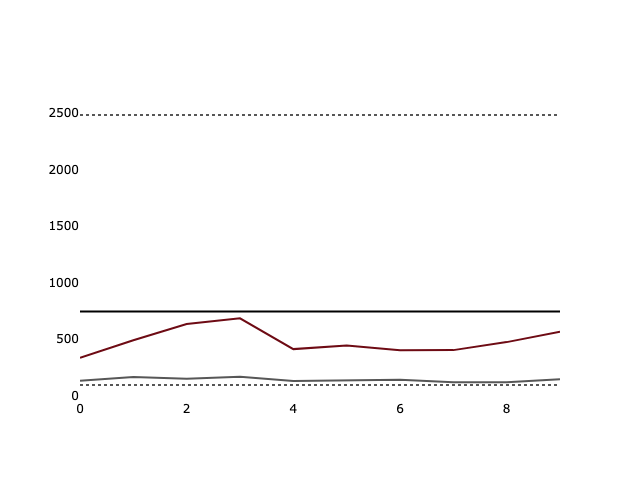
\includegraphics[width=\linewidth]{plots/prompt_1/prompt_1-command_r-cnn_dailymail/prompt_1-command_r-cnn_dailymail_t_word.png}
        \caption{Command-R+\\Total Words}\label{fig-command-r-t-word}
    \end{minipage}
    \hfill
    \begin{minipage}{0.32\textwidth}
        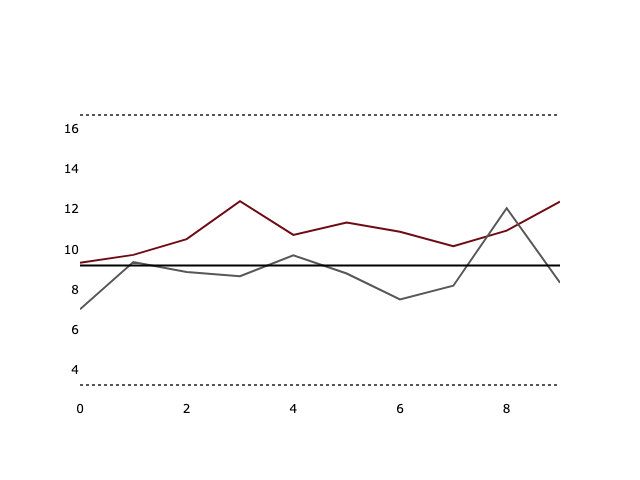
\includegraphics[width=\linewidth]{plots/prompt_1/prompt_1-gpt-cnn_dailymail/prompt_1-gpt-cnn_dailymail_fkgl.png}
        \caption{GPT\\Flesch-Kincaid Grade Level}\label{fig-gpt-fkgl}
    \end{minipage}
    \hfill
    \begin{minipage}{0.32\textwidth}
        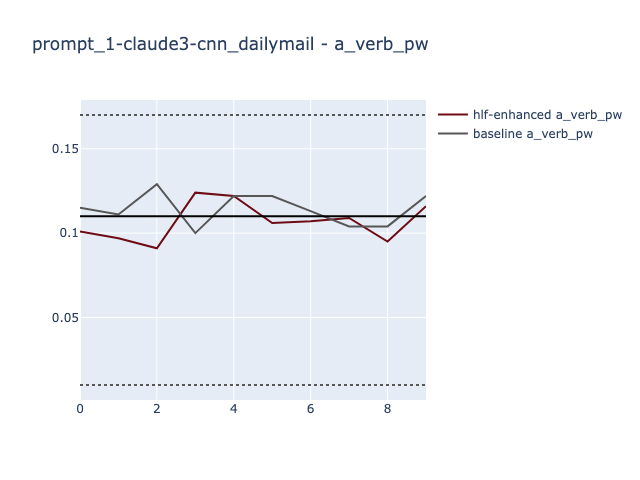
\includegraphics[width=\linewidth]{plots/prompt_1/prompt_1-claude3-cnn_dailymail/prompt_1-claude3-cnn_dailymail_a_verb_pw.png}
        \caption[center]{Claude3\\Average Verbs per Word}\label{fig-llama-simp-ttr}
    \end{minipage}
\end{figure*}

\subsection{HLF Instructions and Context Awareness}

We attempt quantifying the impact of using HLF instructions on the output of the
LLM by eliminating as many factors as possible that would lead to a different
text being generated when compared to a baseline.
In the second scenario of our experiment we use examples to allow the LLM to
generate better baselines, thus hopefully narrowing the gap between baseline
and HLF-enhanced result.

There are two variants of this scenario depending on the provenance of the input
text.
The input text may be from outside the corpus or a text from within the corpus.
Table~\ref{table-prompt-2-cnn-dailymail} contains results for the first variant:
input from outside the corpus.
We notice the HLF results tend to be closer to the target than the baseline
results.
This picture is similar to the one we saw in the first scenario.

\begin{table*}[ht!]
    \centering
    \resizebox{\textwidth}{!}{%
        \begin{tabular}{lllllllllll}
            model                 & t\_word                      & t\_sent                    & n\_uverb                    & n\_uadj                    & simp\_ttr                 & a\_verb\_pw               & corr\_adj\_var            & corr\_verb\_var           & fkgl                       & a\_kup\_pw                \\
            \toprule
            claude3 $Diff_N$     & \textbf{\underline{718.49}}  & \textbf{\underline{24.13}} & \textbf{\underline{44.43}}  & \textbf{\underline{23.43}} & \textbf{\underline{0.4}}  & 0.03                      & 0.94                      & \textbf{\underline{0.77}} & 1.2                        & 0.07                      \\ \midrule
            claude3 $Diff_A$     & \textbf{\underline{2345.54}} & \textbf{\underline{90.18}} & \textbf{\underline{148.36}} & \textbf{\underline{63.6}}  & \textbf{\underline{1.18}} & 0.07                      & 1.36                      & \textbf{\underline{2.55}} & 3.33                       & 0.52                      \\ \midrule
            gemini $Diff_N$      & \textbf{\underline{785.6}}   & \textbf{\underline{25.8}}  & \textbf{\underline{60.5}}   & \textbf{\underline{41.6}}  & \textbf{\underline{0.41}} & \textbf{\underline{0.05}} & \textbf{\underline{1.95}} & \textbf{\underline{2.67}} & -4.62                      & \textbf{\textit{-1.94}}   \\ \midrule
            gemini $Diff_A$      & \textbf{\underline{2512.0}}  & \textbf{\underline{81.5}}  & \textbf{\underline{210.34}} & \textbf{\underline{125.7}} & \textbf{\underline{1.25}} & \textbf{\underline{0.09}} & \textbf{\underline{5.84}} & \textbf{\underline{8.05}} & -9.46                      & \textbf{\textit{-5.82}}   \\ \midrule
            gpt $Diff_N$         & 47.8                         & 5.18                       & 6.13                        & -0.13                      & 0.02                      & 0.0                       & 0.05                      & 0.3                       & 3.06                       & -0.27                     \\ \midrule
            gpt $Diff_A$         & 77.0                         & 12.5                       & 13.0                        & -4.0                       & 0.04                      & 0.0                       & -0.17                     & 0.77                      & 8.45                       & -0.16                     \\ \midrule
            command\_r $Diff_N$  & \textbf{\underline{263.51}}  & 5.35                       & \textbf{\underline{25.08}}  & \textbf{\underline{17.37}} & \textbf{\textit{-0.09}}   & -0.01                     & \textbf{\underline{1.74}} & \textbf{\underline{1.42}} & \textbf{\underline{10.46}} & \textbf{\underline{1.56}} \\ \midrule
            command\_r $Diff_A$  & \textbf{\underline{896.0}}   & 20.5                       & \textbf{\underline{86.0}}   & \textbf{\underline{60.6}}  & \textbf{\textit{-0.21}}   & -0.03                     & \textbf{\underline{5.45}} & \textbf{\underline{4.95}} & \textbf{\underline{31.29}} & \textbf{\underline{5.67}} \\ \midrule
            llama3\_70b $Diff_N$ & \textbf{\underline{376.0}}   & \textbf{\underline{15.63}} & \textbf{\underline{38.63}}  & 15.74                      & \textbf{\underline{0.24}} & \textbf{\underline{0.06}} & 1.69                      & \textbf{\underline{2.91}} & 0.31                       & -0.3                      \\ \midrule
            llama3\_70b $Diff_A$ & \textbf{\underline{1088.5}}  & \textbf{\underline{45.0}}  & \textbf{\underline{113.0}}  & 41.0                       & \textbf{\underline{0.65}} & \textbf{\underline{0.18}} & 3.53                      & \textbf{\underline{8.56}} & 0.27                       & -0.68                     \\ \bottomrule
        \end{tabular}%
    }
    \caption{prompt 2 - CNN Results\\Input Outside Corpus}\label{table-prompt-2-cnn-dailymail} % chktex-file 8
\end{table*}

On the other hand, there are fewer significant differences between baseline and
HLF results.
A possible explanation for this situation might lie in the closeness of the
input prompt (which contains examples from the corpus)to the target.
As we can see in Figure~\ref{fig-p2-gpt-twords}, this is not always the case.
In~\cref{fig-p2-command-r-simpttr,fig-p2-gemini-a-kup-pw} we observe regressions
in performance with significant differences between baseline and result.
Even so, the results obtained in our first scenario are largely confirmed in the
first variant of our second scenario.

\begin{figure*}[ht!]
    \centering
    \begin{minipage}{0.32\textwidth}
        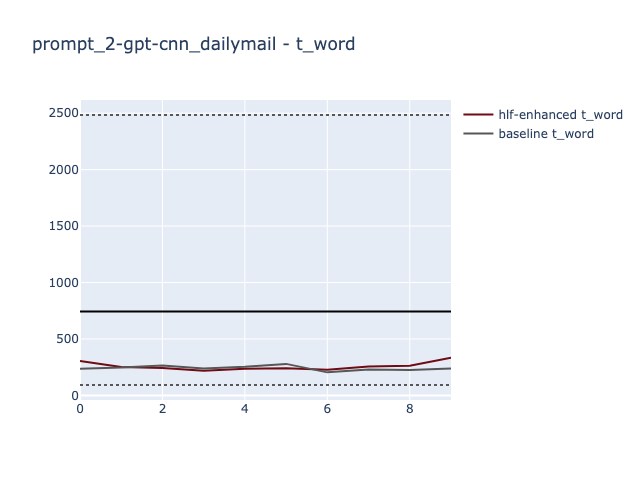
\includegraphics[width=\linewidth]{plots/prompt_2/prompt_2-gpt-cnn_dailymail/prompt_2-gpt-cnn_dailymail_t_word.png}
        \caption{GPT\\Total Words}\label{fig-p2-gpt-twords}
    \end{minipage}
    \hfill
    \begin{minipage}{0.32\textwidth}
        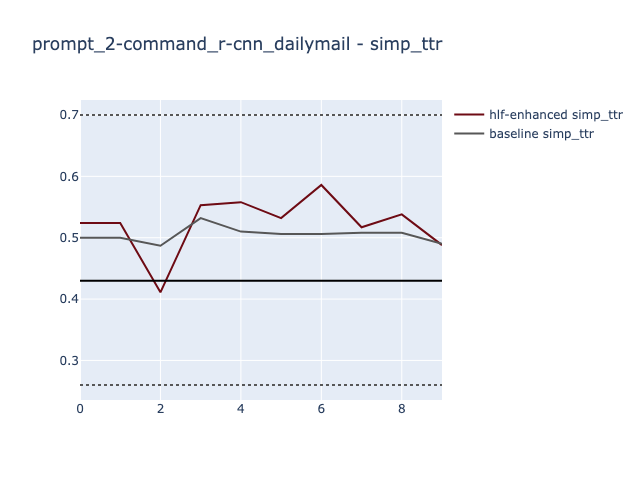
\includegraphics[width=\linewidth]{plots/prompt_2/prompt_2-command_r-cnn_dailymail/prompt_2-command_r-cnn_dailymail_simp_ttr.png}
        \caption{Command-R+\\Simple TTR}\label{fig-p2-command-r-simpttr}
    \end{minipage}
    \hfill
    \begin{minipage}{0.32\textwidth}
        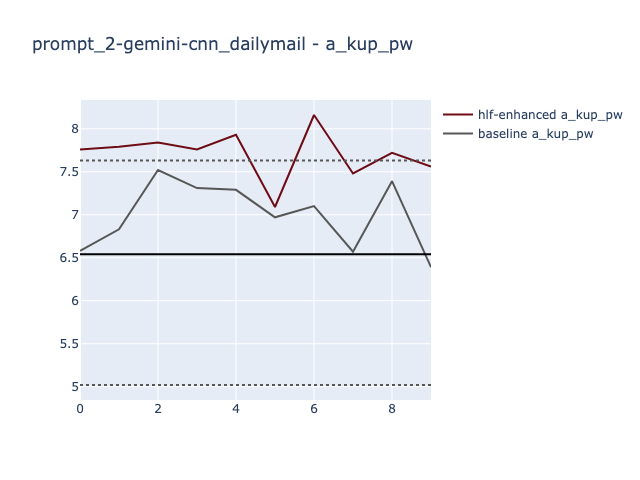
\includegraphics[width=\linewidth]{plots/prompt_2/prompt_2-gemini-cnn_dailymail/prompt_2-gemini-cnn_dailymail_a_kup_pw.png}
        \caption[center]{Gemini\\Kuperman Age of Acquisition}\label{fig-p2-gemini-a-kup-pw}
    \end{minipage}
\end{figure*}

We finally look at the second variant of the second scenario of our experiment.
The hypothesis in this scenario variant was that the baseline would exhibit HLFs
that are much closer to the target corpus average if the input text is from that
corpus.
The expectation is to see fewer significant HLF results and that, as a rule of
thumb, HLF results are closer to the baseline in all cases.
The results shown in Table~\ref{table-prompt-2-ifd-cnn-dailymail} contradict our
expectations outright.
The most surprising behaviour is exhibited for HLFs which are derived into more
concrete generation instructions, such as the total number of words.
This behaviour is highlighted in Figure~\ref{fig-p2-ifd-gemini-twords}.
Additionally, we notice regressive behaviour for some models compared to the
previously explored results in Figure~\ref{fig-p2-ifd-claude3-nuadj}.
Finally, the abstractness of the text generation instructions for certain HLFs
leads to the generated text not being compliant as exemplified in
Figure~\ref{fig-p2-ifd-llama3-a-kup-pw}.

\begin{table*}[ht]
    \centering
    \resizebox{\textwidth}{!}{%
        \begin{tabular}{lllllllllll}
            model                 & t\_word                      & t\_sent                     & n\_uverb                    & n\_uadj                    & simp\_ttr                 & a\_verb\_pw               & corr\_adj\_var             & corr\_verb\_var            & fkgl                       & a\_kup\_pw              \\
            \toprule
            claude3 $Diff_N$     & \textbf{\underline{871.02}}  & \textbf{\underline{34.2}}   & \textbf{\underline{34.48}}  & \textbf{\textit{-7.38}}    & \textbf{\underline{0.27}} & 0.01                      & \textbf{\textit{-0.93}}    & \textbf{\textit{-0.72}}    & 1.16                       & -0.14                   \\ \midrule
            claude3 $Diff_A$     & \textbf{\underline{2756.12}} & \textbf{\underline{117.18}} & \textbf{\underline{126.36}} & \textbf{\textit{-11.2}}    & \textbf{\underline{0.81}} & -0.01                     & \textbf{\textit{-2.52}}    & \textbf{\textit{-0.74}}    & 3.69                       & -0.4                    \\ \midrule
            gemini $Diff_N$      & \textbf{\underline{1315.41}} & \textbf{\underline{46.19}}  & \textbf{\underline{114.47}} & \textbf{\underline{72.38}} & \textbf{\underline{1.17}} & 0.03                      & \textbf{\underline{5.25}}  & \textbf{\underline{6.64}}  & -1.6                       & \textbf{\textit{-2.1}}  \\ \midrule
            gemini $Diff_A$      & \textbf{\underline{3996.0}}  & \textbf{\underline{138.0}}  & \textbf{\underline{357.36}} & \textbf{\underline{212.7}} & \textbf{\underline{3.3}}  & 0.06                      & \textbf{\underline{15.49}} & \textbf{\underline{19.4}}  & -13.22                     & \textbf{\textit{-6.19}} \\ \midrule
            gpt $Diff_N$         & \textbf{\underline{521.29}}  & \textbf{\underline{23.3}}   & \textbf{\underline{43.13}}  & 19.85                      & \textbf{\underline{0.2}}  & 0.02                      & 1.08                       & \textbf{\underline{1.04}}  & 5.09                       & 0.67                    \\ \midrule
            gpt $Diff_A$         & \textbf{\underline{1464.0}}  & \textbf{\underline{65.5}}   & \textbf{\underline{121.84}} & 58.1                       & \textbf{\underline{0.58}} & 0.05                      & 2.93                       & \textbf{\underline{2.59}}  & 14.23                      & 1.89                    \\ \midrule
            command\_r $Diff_N$  & \textbf{\underline{371.08}}  & \textbf{\underline{13.31}}  & 22.06                       & \textbf{\underline{17.19}} & \textbf{\underline{0.17}} & \textbf{\underline{0.02}} & 0.88                       & 1.09                       & \textbf{\underline{4.05}}  & -0.15                   \\ \midrule
            command\_r $Diff_A$  & \textbf{\underline{1198.0}}  & \textbf{\underline{42.5}}   & 73.0                        & \textbf{\underline{56.5}}  & \textbf{\underline{0.69}} & \textbf{\underline{0.07}} & 2.85                       & 3.99                       & \textbf{\underline{13.89}} & -0.11                   \\ \midrule
            llama3\_70b $Diff_N$ & \textbf{\underline{1040.85}} & \textbf{\underline{41.99}}  & \textbf{\underline{80.58}}  & \textbf{\underline{49.12}} & \textbf{\underline{0.55}} & \textbf{\underline{0.04}} & \textbf{\underline{3.99}}  & \textbf{\underline{5.05}}  & 7.18                       & \textbf{\textit{-1.94}} \\ \midrule
            llama3\_70b $Diff_A$ & \textbf{\underline{2928.0}}  & \textbf{\underline{118.5}}  & \textbf{\underline{222.0}}  & \textbf{\underline{133.5}} & \textbf{\underline{1.43}} & \textbf{\underline{0.05}} & \textbf{\underline{10.77}} & \textbf{\underline{13.42}} & 17.21                      & \textbf{\textit{-6.2}}  \\ \bottomrule
        \end{tabular}%
    }
    \caption{CNN Results\\Input Inside Corpus}\label{table-prompt-2-ifd-cnn-dailymail}
\end{table*}

\begin{figure*}[ht!]
    \centering
    \begin{minipage}{0.32\textwidth}
        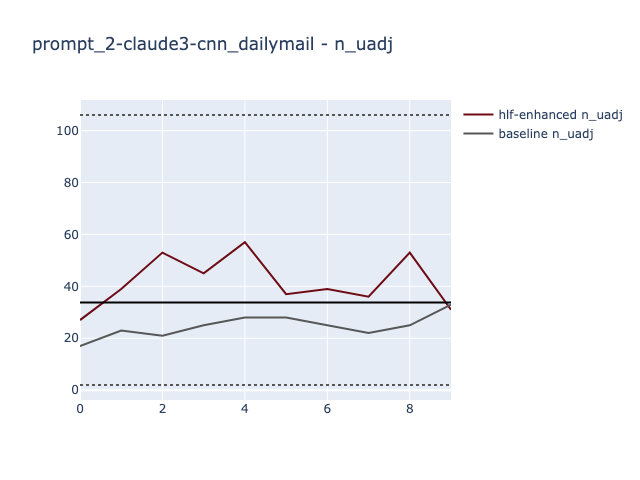
\includegraphics[width=\linewidth]{plots/prompt_2_ifd/prompt_2-claude3-cnn_dailymail/prompt_2-claude3-cnn_dailymail_n_uadj.png}
        \caption{Claude3\\Number of Unique Adjectives}\label{fig-p2-ifd-claude3-nuadj}
    \end{minipage}
    \hfill
    \begin{minipage}{0.32\textwidth}
        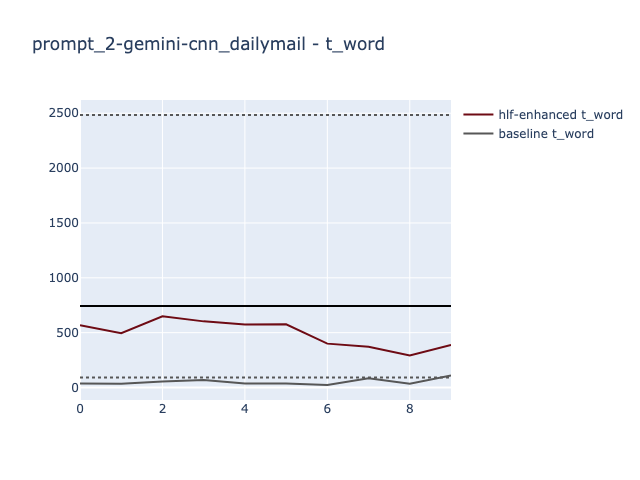
\includegraphics[width=\linewidth]{plots/prompt_2_ifd/prompt_2-gemini-cnn_dailymail/prompt_2-gemini-cnn_dailymail_t_word.png}
        \caption{Gemini\\Total Words}\label{fig-p2-ifd-gemini-twords}
    \end{minipage}
    \hfill
    \begin{minipage}{0.32\textwidth}
        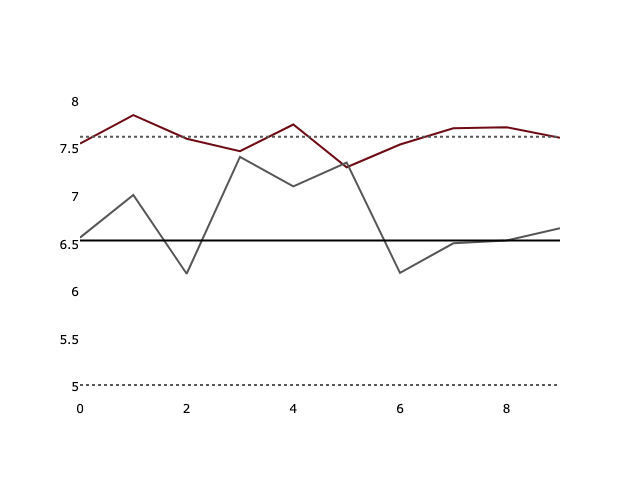
\includegraphics[width=\linewidth]{plots/prompt_2_ifd/prompt_2-llama3_70b-cnn_dailymail/prompt_2-llama3_70b-cnn_dailymail_a_kup_pw.png}
        \caption[center]{Llama3\\Kuperman Age of Acquisition}\label{fig-p2-ifd-llama3-a-kup-pw}
    \end{minipage}
\end{figure*}

Overall, the LLMs do not seem to utilize the examples given in the prompt to
their advantage when generating text that should mirror the linguistic features
of those examples.

\section{Discussion}

In terms of our first question --- whether HLF instructions impact an LLM's
writing, the response is affirmative.
Not all LLMs are equally susceptible to HLF instructions, though.
The experiment design involves choices that rely on the presence of a corpus and
the usage of a fixed external input text.
This is relevant as evidentiated by the difference in HLF results obtained using
the Yelp reviews corpus when compared to the HLF results obtained on the CNN
article corpus.
While similarly significant, the HLF results on Yelp reviews are mostly worse
than their corresponding baselines failing to confirm the positive impact of HLF
instructions.
The importance of the choice of the external text is highlighted by the better
HLF results obtained using an input text from the corpus.

Let us move on to how much HLF instructions impact an LLM's writing.
The metrics we compute dismiss the idea that HLF instructions have a consistent
desired impact on the generated text.
There isn't conclusive evidence that if we improve the LLM's chances of
producing a better baseline, this will result in a smaller difference between
baseline and HLF result relative to the target HLF.
In fact, there is evidence that HLF instructions have an adverse effect when
examining the HLF results obtained on the Yelp reviews dataset.
This is especially true of highly abstract HLF instructions.
LLMs do not seem to follow these instructions well in most scenarios.
The impact of highly abstract HLF instructions tends to be adverse.

The choice of input text in relation to the target HLF values is consequential.
LLMs don't yet seem able to cover the gulf between Oscar Wilde poems and the
average Yelp review in terms of linguistic features.
We surmise that even if LLMs are able to generate text that complies to certain
target HLFs, there is a limit to this ability.

\section{Limitations and Future Work}

Other experiments are required to better understand the capabilities of large
language models with regard to HLFs.
The selection of language models, the reliance on a corpus for computing target
linguistic features, the fixed choice of input text are all limitations of the
current approach.
Making different experiment design choices in all these respects might shed more
light on this matter.
Using a selection of HLFs and not individually analysing the behaviour of the
LLM under the influence of each individual HLF is another limiting choice that
invites to future work on the alternative.

\section{Conclusions}

We began by trying to understand whether it is possible to generate text that
exhibits certain linguistic features by instructing a large language model.
It turns out state of the art large language models are receptive to
instructions regarding the linguistic features of the output.
This is especially true for concrete instructions.

However, the outcomes are not always good.
From a pragmatic standpoint, prompt engineering and a careful choice of language
features and input text seem like the way to obtain desirable results.
Providing examples in the input prompt does not seem to influence the HLFs of
the LLM output in the expected manner.

Finally, we've seen how we might use handcrafted linguistic features to assess
LLM output.
Setting up ``before and after'' scenarios to evaluate relative improvements of
the LLM outcome in relation to the selected HLFs is one way to achieve this.
Given enough measurements, the relative difference between the exhibited
baseline and target HLFs can be quantified relatively easily using geometric or
statistical means.

\bibliography{references}

\appendix

\section{Additional Result Tables}\label{sec:yelp-tables}
\subsection{Yelp}
\Cref{table-prompt-1-yelp,table-prompt-2-yelp,table-prompt-2-ifd-yelp} show the
experiment results on the corpus of reviews extracted from the Yelp dataset.

\begin{table*}[ht]
    \centering
    \resizebox{\textwidth}{!}{%
        \begin{tabular}{lllllllllll}
            model                 & t\_word                   & t\_sent                    & n\_uverb                 & n\_uadj                  & simp\_ttr & a\_verb\_pw             & corr\_adj\_var          & corr\_verb\_var         & fkgl                       & a\_kup\_pw               \\
            \toprule
            claude3 $Diff_N$     & \textbf{\textit{-281.9}}  & \textbf{\textit{-13.22}}   & \textbf{\textit{-25.79}} & -14.56                   & -0.06     & 0.0                     & -1.27                   & -1.14                   & \textbf{\underline{6.89}}  & \textbf{\underline{1.0}} \\ \midrule
            claude3 $Diff_A$     & \textbf{\textit{-774.0}}  & \textbf{\textit{-27.76}}   & \textbf{\textit{-70.0}}  & -38.0                    & -0.19     & 0.02                    & -3.25                   & -3.39                   & \textbf{\underline{21.68}} & \textbf{\underline{2.9}} \\ \midrule
            gemini $Diff_N$      & -109.27                   & 0.05                       & -7.25                    & -13.18                   & -0.14     & 0.01                    & -1.01                   & -0.4                    & 1.62                       & -0.4                     \\ \midrule
            gemini $Diff_A$      & -252.82                   & -0.78                      & -17.5                    & -23.14                   & -0.52     & 0.01                    & -1.85                   & -1.07                   & 7.14                       & -0.93                    \\ \midrule
            gpt $Diff_N$         & -21.62                    & 2.42                       & -3.8                     & -8.84                    & 0.0       & -0.01                   & -0.8                    & -0.53                   & 8.94                       & -0.37                    \\ \midrule
            gpt $Diff_A$         & -34.72                    & 9.68                       & -10.54                   & -24.57                   & -0.03     & -0.02                   & -2.37                   & -1.58                   & 19.26                      & -1.03                    \\ \midrule
            command\_r $Diff_N$  & -40.1                     & 1.22                       & 2.43                     & \textbf{\textit{-13.64}} & 0.05      & \textbf{\textit{-0.04}} & \textbf{\textit{-1.17}} & 0.59                    & \textbf{\textit{-7.25}}    & \textbf{\textit{-1.67}}  \\ \midrule
            command\_r $Diff_A$  & -75.5                     & 1.5                        & 12.94                    & \textbf{\textit{-34.0}}  & 0.19      & \textbf{\textit{-0.12}} & \textbf{\textit{-2.76}} & 2.83                    & \textbf{\textit{-20.49}}   & \textbf{\textit{-4.76}}  \\ \midrule
            llama3\_70b $Diff_N$ & \textbf{\textit{-210.45}} & \textbf{\underline{6.87}}  & \textbf{\textit{-13.46}} & \textbf{\textit{-15.17}} & -0.16     & \textbf{\textit{-0.02}} & \textbf{\textit{-1.78}} & \textbf{\textit{-1.31}} & 3.7                        & \textbf{\textit{-1.58}}  \\ \midrule
            llama3\_70b $Diff_A$ & \textbf{\textit{-607.52}} & \textbf{\underline{19.42}} & \textbf{\textit{-41.22}} & \textbf{\textit{-44.77}} & -0.42     & \textbf{\textit{-0.05}} & \textbf{\textit{-5.48}} & \textbf{\textit{-4.34}} & 9.79                       & \textbf{\textit{-4.98}}  \\ \bottomrule
        \end{tabular}%
    }
    \caption{Yelp Results - Prompt Without Examples}\label{table-prompt-1-yelp} % chktex-file 8
\end{table*}

\begin{table*}[!ht]
    \centering
    \resizebox{\textwidth}{!}{%
        \begin{tabular}{lllllllllll}
            model                 & t\_word & t\_sent & n\_uverb & n\_uadj & simp\_ttr & a\_verb\_pw & corr\_adj\_var            & corr\_verb\_var & fkgl                       & a\_kup\_pw \\
            \toprule
            claude3 $Diff_N$     & -121.77 & -4.61   & -9.9     & 18.41   & -0.11     & 0.03        & \textbf{\underline{1.4}}  & -0.33           & 1.81                       & 0.95       \\ \midrule
            claude3 $Diff_A$     & -394.5  & -11.5   & -37.5    & 60.0    & -0.37     & 0.09        & \textbf{\underline{4.66}} & -1.49           & 5.38                       & 2.62       \\ \midrule
            gemini $Diff_N$      & -23.49  & 1.52    & -0.55    & -1.29   & -0.02     & -0.01       & 0.09                      & -0.05           & \textbf{\underline{6.41}}  & 0.2        \\ \midrule
            gemini $Diff_A$      & -83.0   & 3.0     & -2.5     & -6.36   & -0.0      & -0.03       & 0.26                      & -0.08           & \textbf{\underline{19.63}} & 0.53       \\ \midrule
            gpt $Diff_N$         & 13.66   & 2.83    & -3.65    & -3.19   & 0.04      & -0.04       & -0.24                     & -0.22           & 7.5                        & 0.0        \\ \midrule
            gpt $Diff_A$         & 55.5    & 9.5     & -9.86    & -12.86  & 0.14      & -0.11       & -0.84                     & -0.22           & 18.67                      & -0.38      \\ \midrule
            command\_r $Diff_N$  & -188.71 & 0.69    & -10.73   & 1.17    & -0.23     & -0.01       & \textbf{\underline{0.74}} & -0.83           & \textbf{\textit{-5.02}}    & -0.08      \\ \midrule
            command\_r $Diff_A$  & -516.82 & 2.02    & -29.22   & 8.28    & -0.66     & -0.0        & \textbf{\underline{2.98}} & -2.48           & \textbf{\textit{-14.52}}   & -0.48      \\ \midrule
            llama3\_70b $Diff_N$ & -202.95 & -7.84   & -13.73   & 1.43    & -0.15     & -0.04       & 0.38                      & -1.39           & 10.67                      & 1.37       \\ \midrule
            llama3\_70b $Diff_A$ & -561.24 & -18.78  & -49.94   & 5.07    & -0.38     & -0.14       & 1.62                      & -4.81           & 29.26                      & 3.11       \\ \bottomrule
        \end{tabular}%
    }
    \caption{Yelp Results - Prompt With Examples\\Input External To Corpus}\label{table-prompt-2-yelp}
\end{table*}
\begin{table*}[!ht]
    \centering
    \resizebox{\textwidth}{!}{%
        \begin{tabular}{lllllllllll}
            model                 & t\_word                   & t\_sent                 & n\_uverb                  & n\_uadj                  & simp\_ttr               & a\_verb\_pw & corr\_adj\_var          & corr\_verb\_var         & fkgl                    & a\_kup\_pw              \\
            \toprule
            claude3 $Diff_N$     & -148.13                   & -1.63                   & -3.93                     & \textbf{\textit{-46.03}} & -0.11                   & -0.0        & \textbf{\textit{-3.08}} & -0.31                   & -4.3                    & \textbf{\textit{-1.53}} \\ \midrule
            claude3 $Diff_A$     & -526.14                   & -7.98                   & -23.86                    & \textbf{\textit{-133.5}} & -0.41                   & -0.0        & \textbf{\textit{-8.98}} & -1.75                   & -21.03                  & \textbf{\textit{-5.34}} \\ \midrule
            gemini $Diff_N$      & 74.27                     & 0.65                    & 4.67                      & 2.98                     & 0.04                    & -0.0        & -0.22                   & 1.05                    & 1.44                    & -0.65                   \\ \midrule
            gemini $Diff_A$      & 221.0                     & 2.0                     & 10.5                      & 7.44                     & 0.12                    & -0.03       & -0.85                   & 2.73                    & 3.28                    & -1.79                   \\ \midrule
            gpt $Diff_N$         & 0.65                      & 4.03                    & -1.19                     & -2.66                    & -0.03                   & -0.01       & -0.17                   & -0.13                   & 1.05                    & -0.67                   \\ \midrule
            gpt $Diff_A$         & 17.0                      & 11.68                   & -3.68                     & -7.0                     & -0.1                    & -0.04       & -0.43                   & -0.05                   & 0.57                    & -1.75                   \\ \midrule
            command\_r $Diff_N$  & \textbf{\textit{-236.11}} & \textbf{\textit{-3.6}}  & \textbf{\textit{-0.97}}   & \textbf{\textit{-27.04}} & \textbf{\textit{-0.23}} & 0.0         & -1.24                   & \textbf{\textit{-1.08}} & \textbf{\textit{-2.13}} & \textbf{\textit{-1.09}} \\ \midrule
            command\_r $Diff_A$  & \textbf{\textit{-727.0}}  & \textbf{\textit{-9.24}} & \textbf{\underline{0.76}} & \textbf{\textit{-68.5}}  & \textbf{\textit{-0.64}} & 0.02        & -2.89                   & \textbf{\textit{-3.08}} & \textbf{\textit{-5.5}}  & \textbf{\textit{-3.0}}  \\ \midrule
            llama3\_70b $Diff_N$ & \textbf{\textit{-333.03}} & \textbf{\textit{-5.19}} & 4.43                      & \textbf{\textit{-21.38}} & -0.16                   & -0.03       & \textbf{\textit{-1.77}} & -0.03                   & 1.87                    & -0.44                   \\ \midrule
            llama3\_70b $Diff_A$ & \textbf{\textit{-687.34}} & \textbf{\textit{-3.42}} & 10.7                      & \textbf{\textit{-61.64}} & -0.31                   & -0.04       & \textbf{\textit{-5.6}}  & -0.89                   & 3.0                     & -1.92                   \\ \bottomrule
        \end{tabular}%
    }
    \caption{Yelp Results - Prompt With Examples\\Input From Corpus}\label{table-prompt-2-ifd-yelp}
\end{table*}

\section{Additional Plots}

\subsection{GPT}

\begin{figure*}[ht]
    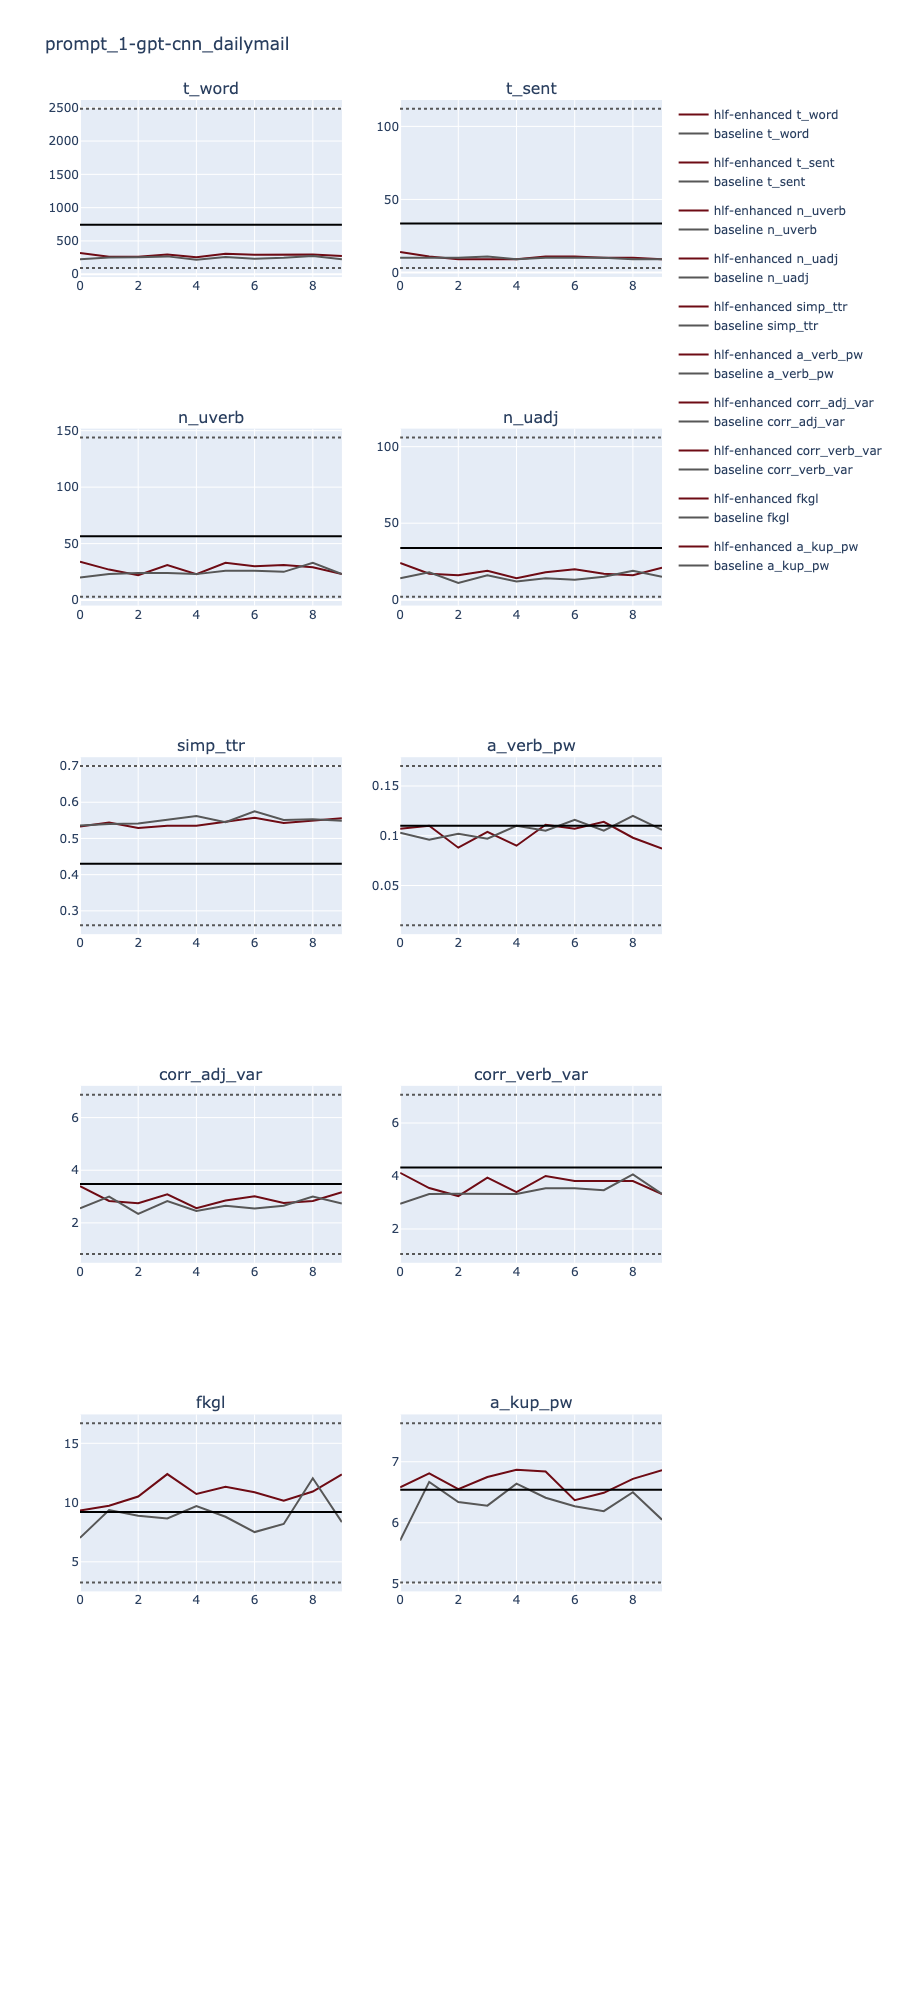
\includegraphics[width=\textwidth,height=0.9\textheight,scale=1]{plots/prompt_1/prompt_1-gpt-cnn_dailymail/prompt_1-gpt-cnn_dailymail.png}
    \caption{GPT on CNN Corpus\\Prompt Without Examples}\label{fig:gpt-prompt1-cnn}
\end{figure*}
\begin{figure*}[ht]
    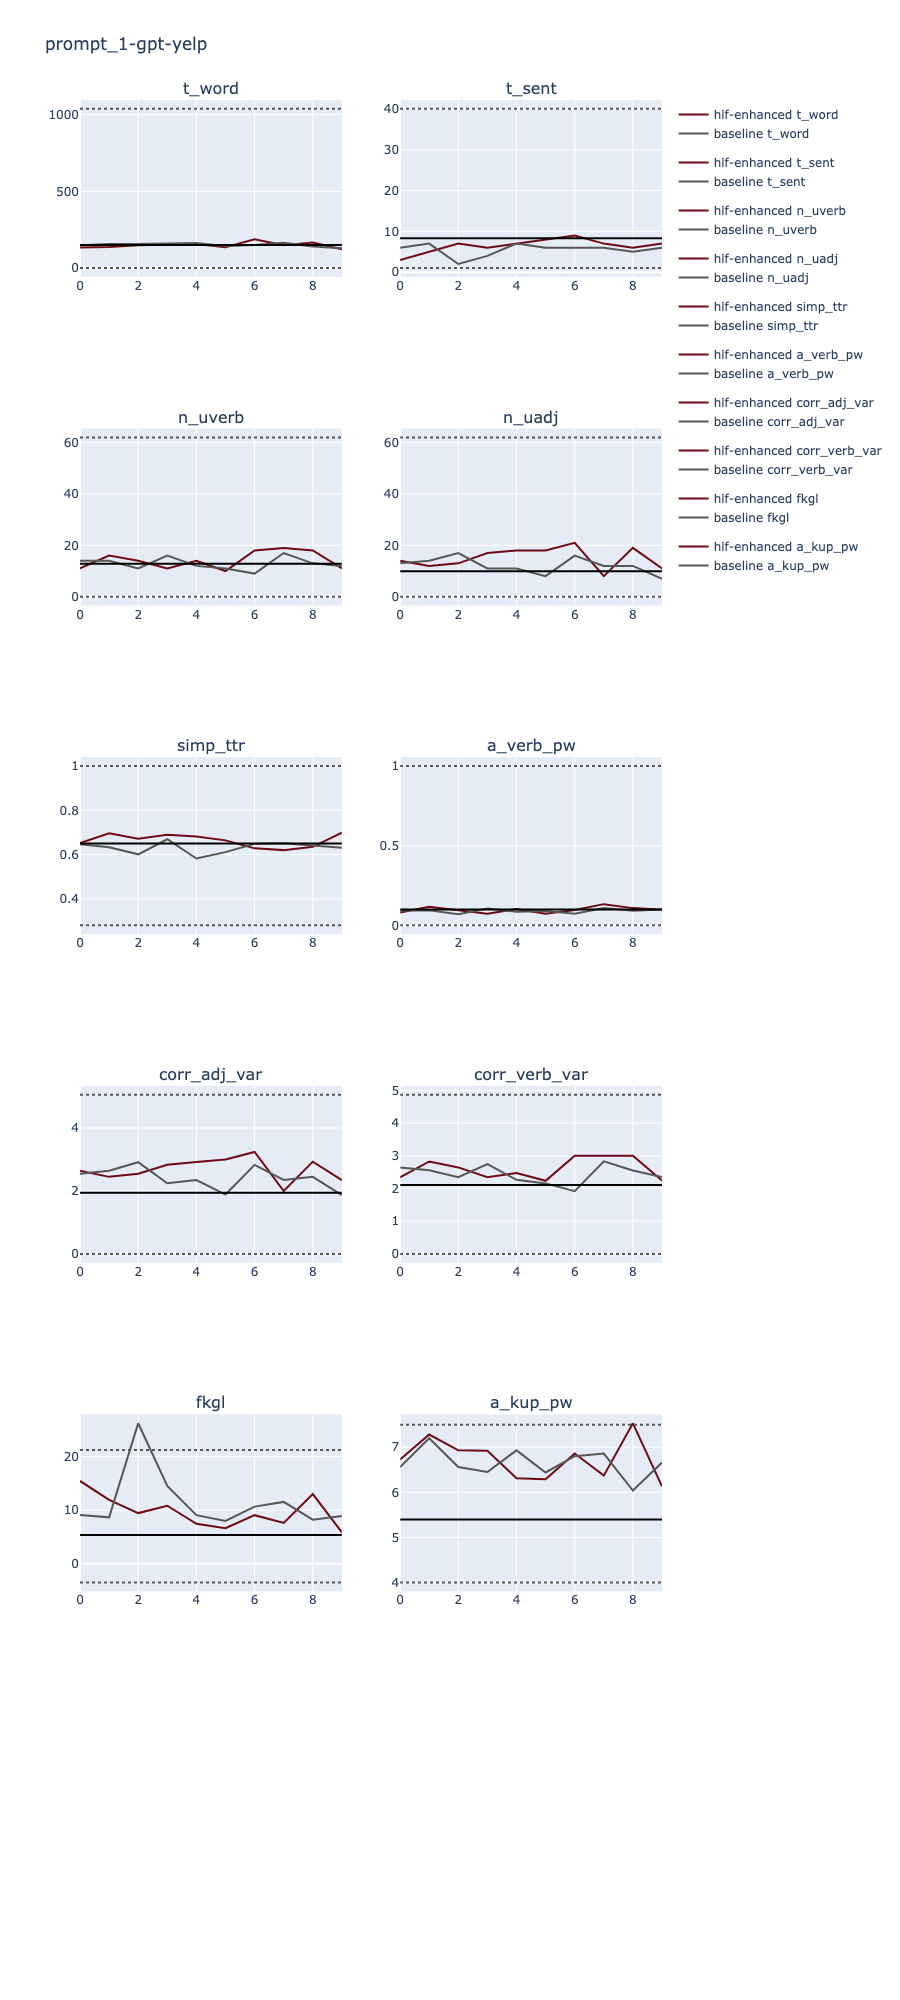
\includegraphics[width=\textwidth,height=0.9\textheight,scale=1]{plots/prompt_1/prompt_1-gpt-yelp/prompt_1-gpt-yelp.png}
    \caption{GPT on Yelp Corpus\\Prompt Without Examples}\label{fig:gpt-prompt1-yelp}
\end{figure*}
\begin{figure*}[ht]
    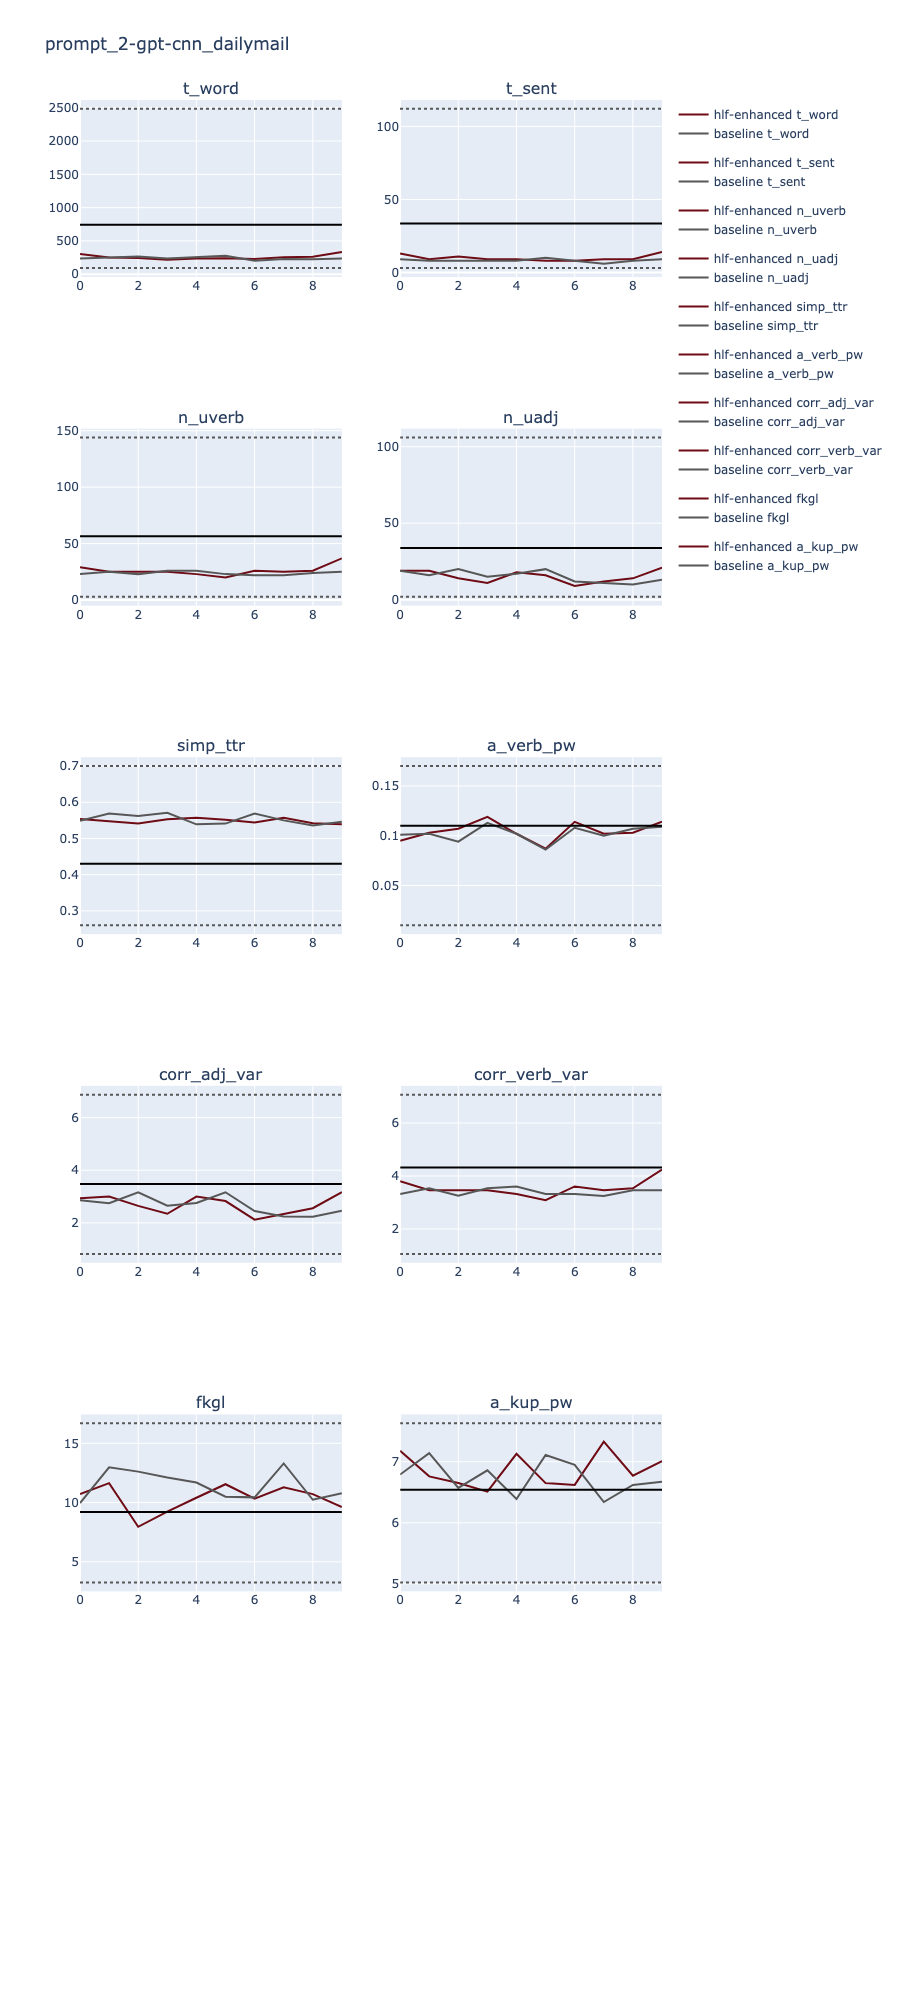
\includegraphics[width=\textwidth,height=0.9\textheight,scale=1]{plots/prompt_2/prompt_2-gpt-cnn_dailymail/prompt_2-gpt-cnn_dailymail.png}
    \caption{GPT on CNN Corpus\\Prompt With Examples\\Extraneous Input}\label{fig:gpt-prompt2-cnn}
\end{figure*}
\begin{figure*}[ht]
    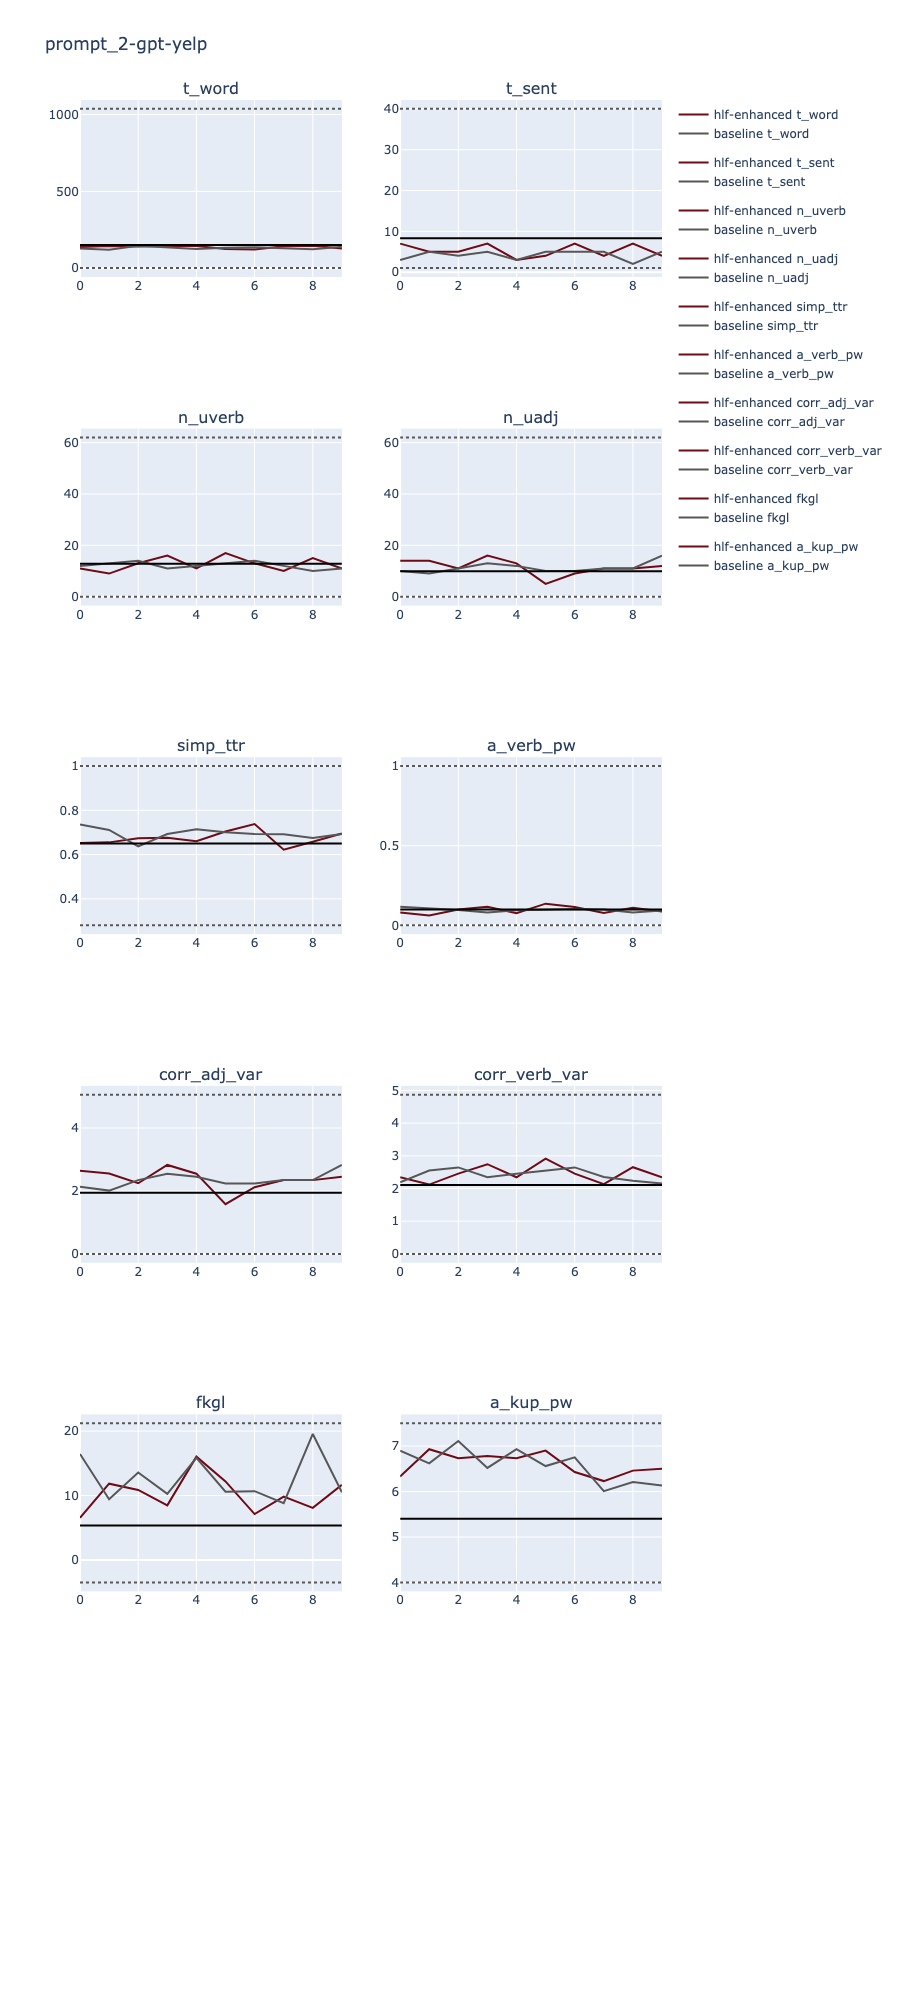
\includegraphics[width=\textwidth,height=0.9\textheight,scale=1]{plots/prompt_2/prompt_2-gpt-yelp/prompt_2-gpt-yelp.png}
    \caption{GPT on Yelp Corpus\\Prompt With Examples\\Extraneous Input}\label{fig:gpt-prompt2-yelp}
\end{figure*}
\begin{figure*}[ht]
    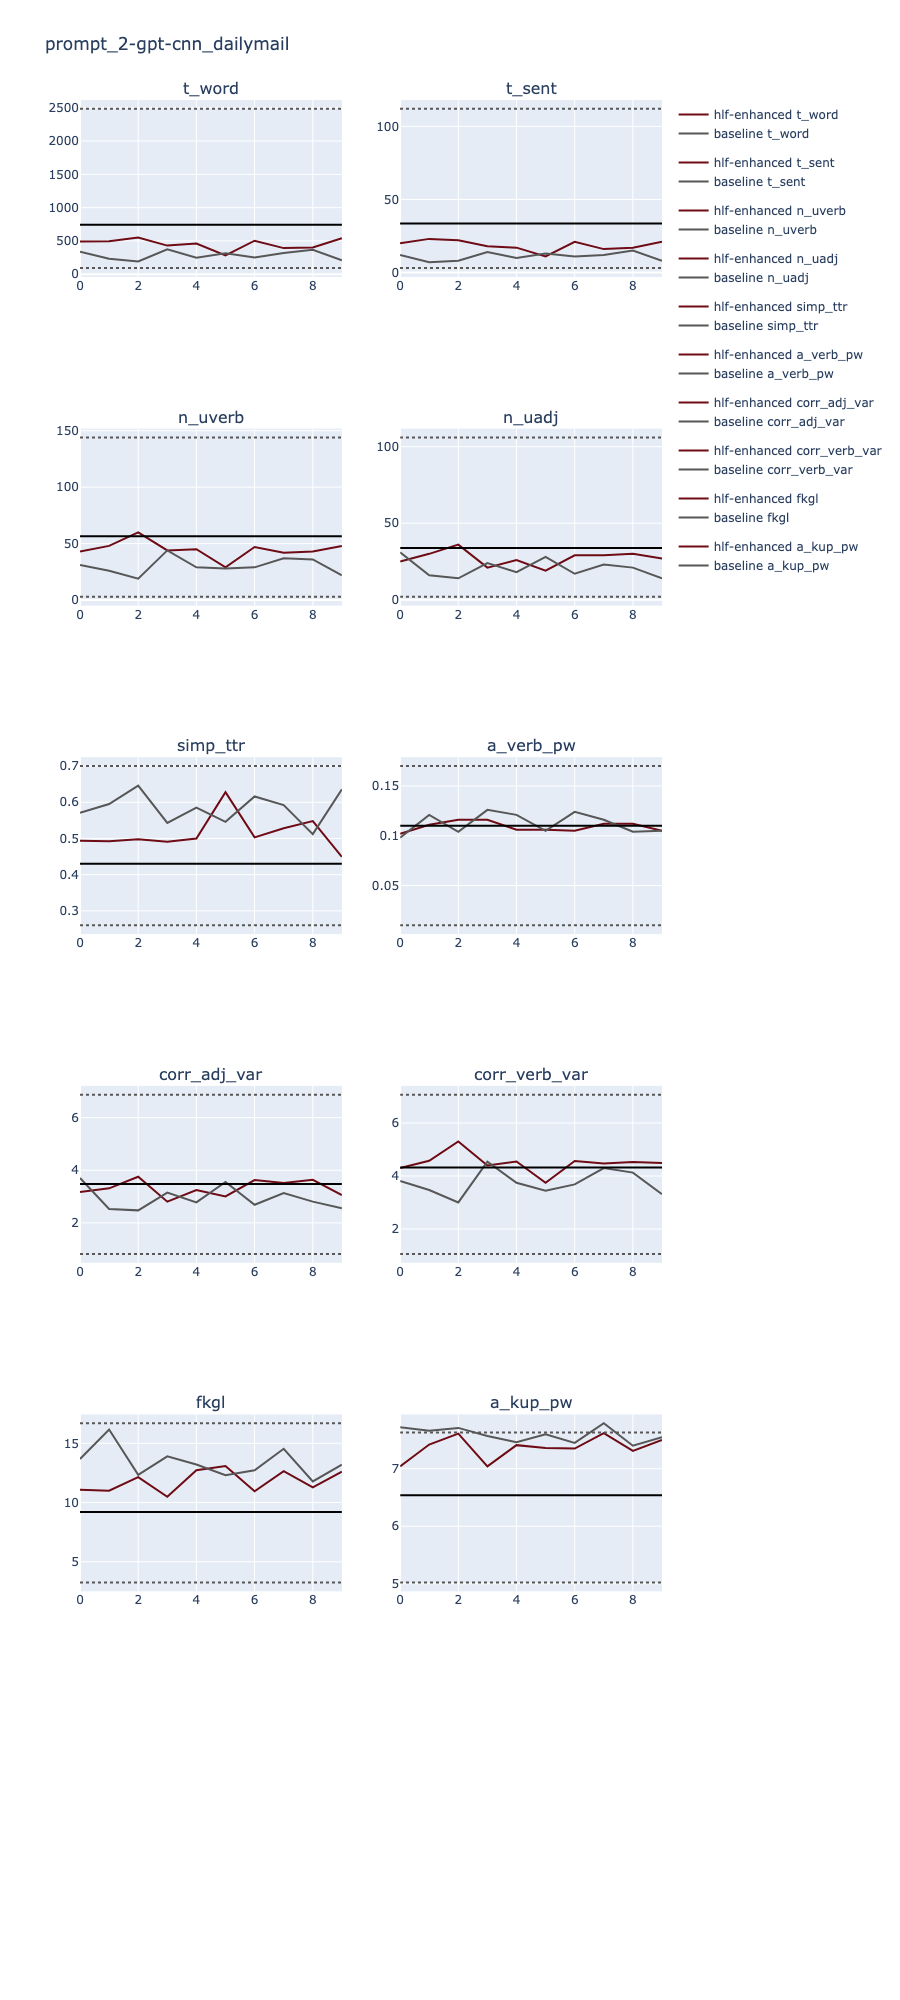
\includegraphics[width=\textwidth,height=0.9\textheight,scale=1]{plots/prompt_2_ifd/prompt_2-gpt-cnn_dailymail/prompt_2-gpt-cnn_dailymail.png}
    \caption{GPT on CNN Corpus\\Prompt With Examples\\Input from Corpus}\label{fig:gpt-prompt2-cnn-ifd}
\end{figure*}
\begin{figure*}[ht]
    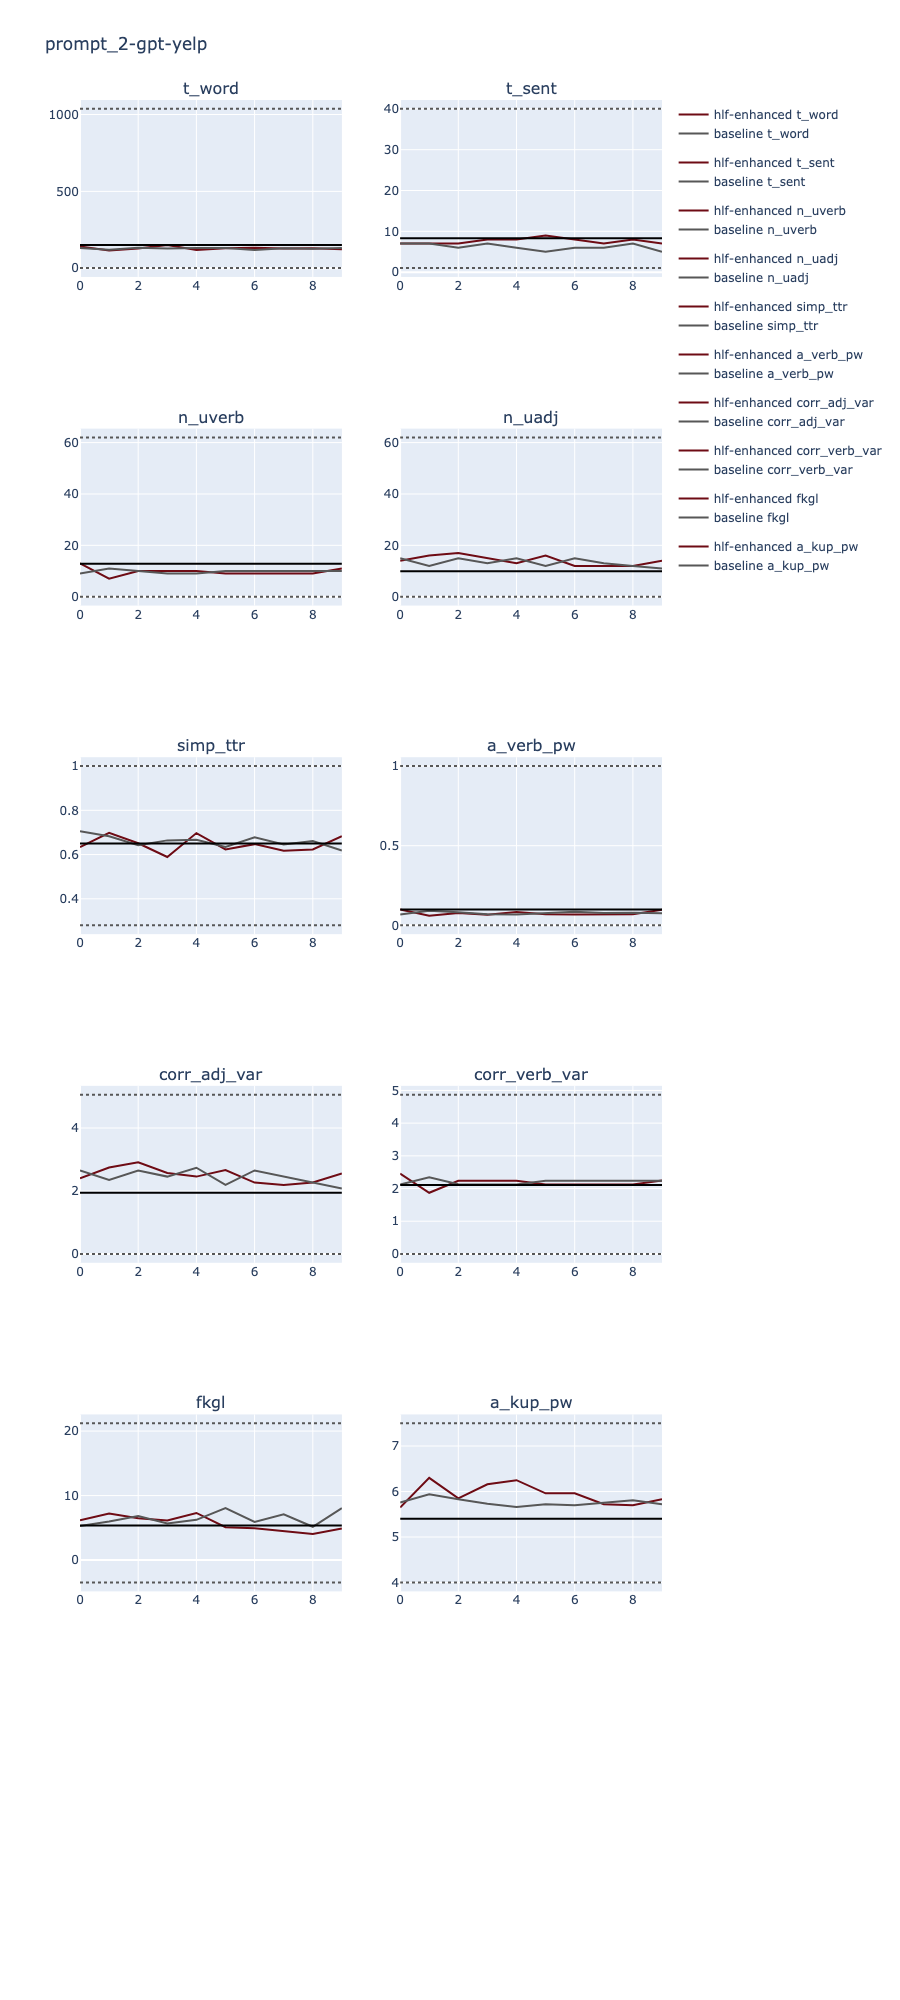
\includegraphics[width=\textwidth,height=0.9\textheight,scale=1]{plots/prompt_2_ifd/prompt_2-gpt-yelp/prompt_2-gpt-yelp.png}
    \caption{GPT on Yelp Corpus\\Prompt With Examples\\Input from Corpus}\label{fig:gpt-prompt2-yelp-ifd}
\end{figure*}

\Cref{fig:gpt-prompt1-cnn,fig:gpt-prompt1-yelp,fig:gpt-prompt2-cnn,fig:gpt-prompt2-yelp,fig:gpt-prompt2-cnn-ifd,fig:gpt-prompt2-yelp-ifd}
show the experiment results for the Claude 3 Opus large language model.

\subsection{Gemini}

\begin{figure*}[ht]
    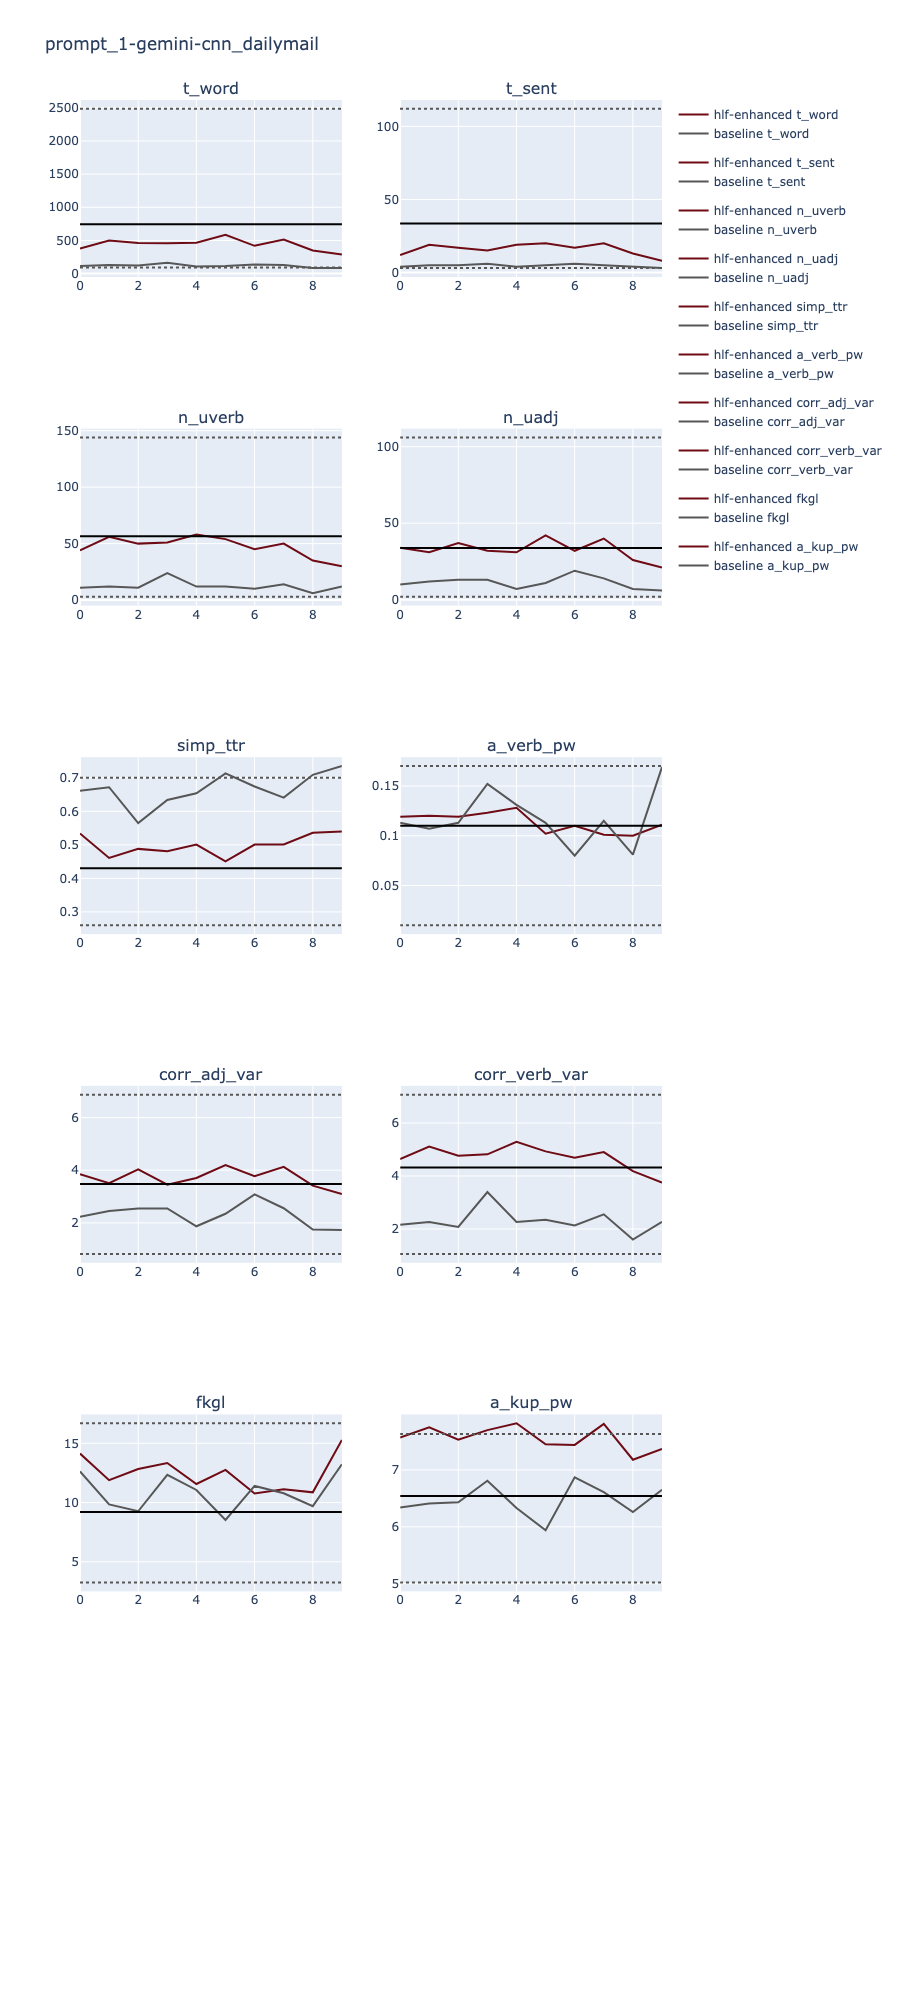
\includegraphics[width=\textwidth,height=0.9\textheight,scale=1]{plots/prompt_1/prompt_1-gemini-cnn_dailymail/prompt_1-gemini-cnn_dailymail.png}
    \caption{Gemini on CNN Corpus\\Prompt Without Examples}\label{fig:gemini-prompt1-cnn}
\end{figure*}
\begin{figure*}[ht]
    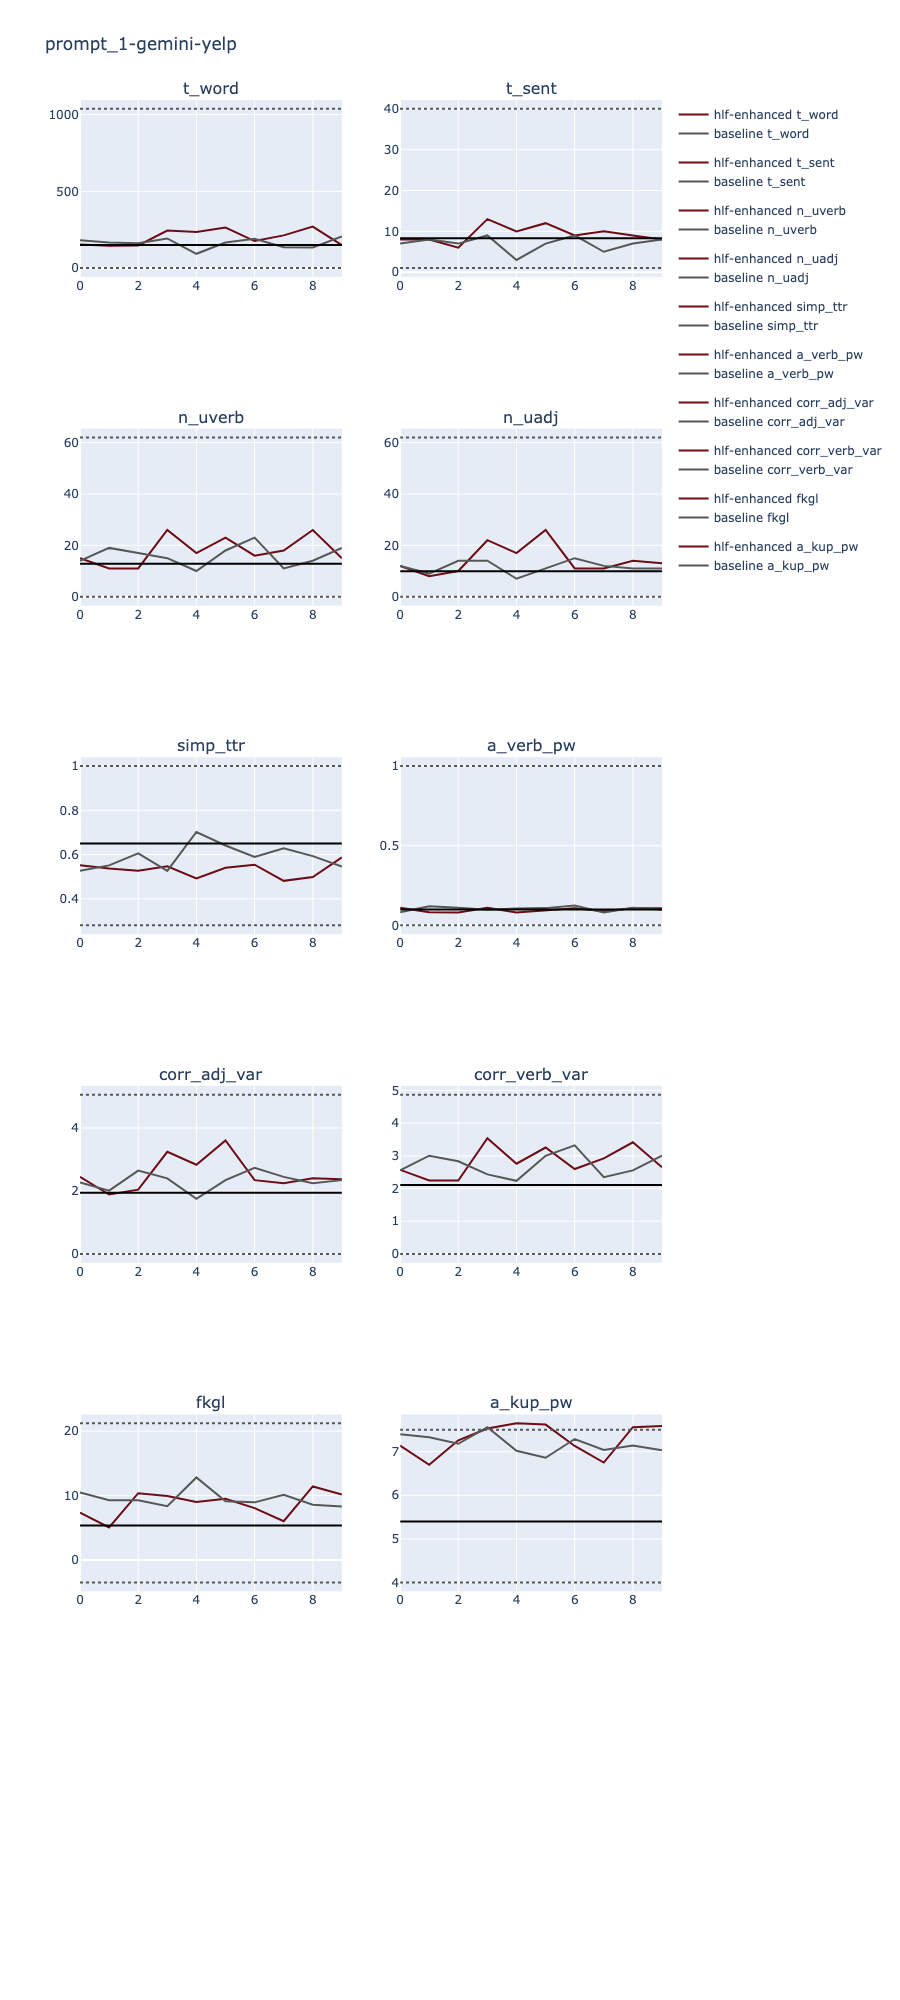
\includegraphics[width=\textwidth,height=0.9\textheight,scale=1]{plots/prompt_1/prompt_1-gemini-yelp/prompt_1-gemini-yelp.png}
    \caption{Gemini on Yelp Corpus\\Prompt Without Examples}\label{fig:gemini-prompt1-yelp}
\end{figure*}
\begin{figure*}[ht]
    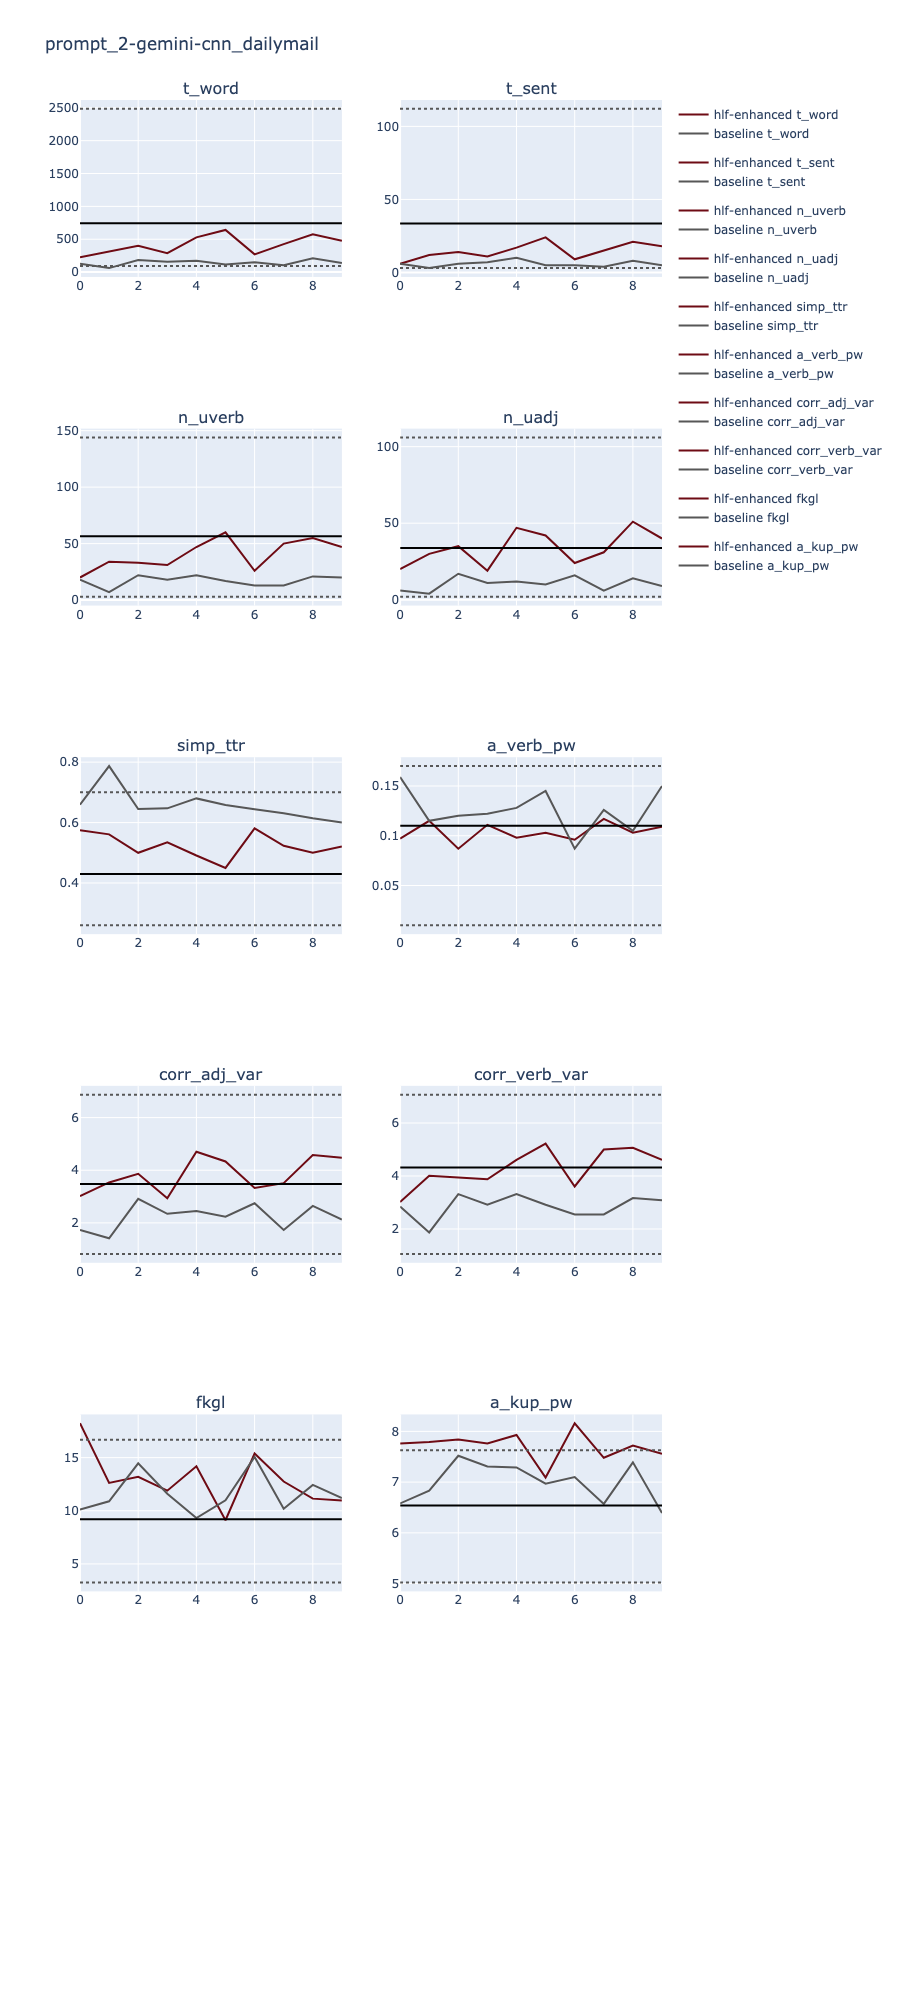
\includegraphics[width=\textwidth,height=0.9\textheight,scale=1]{plots/prompt_2/prompt_2-gemini-cnn_dailymail/prompt_2-gemini-cnn_dailymail.png}
    \caption{Gemini on CNN Corpus\\Prompt With Examples\\Extraneous Input}\label{fig:gemini-prompt2-cnn}
\end{figure*}
\begin{figure*}[ht]
    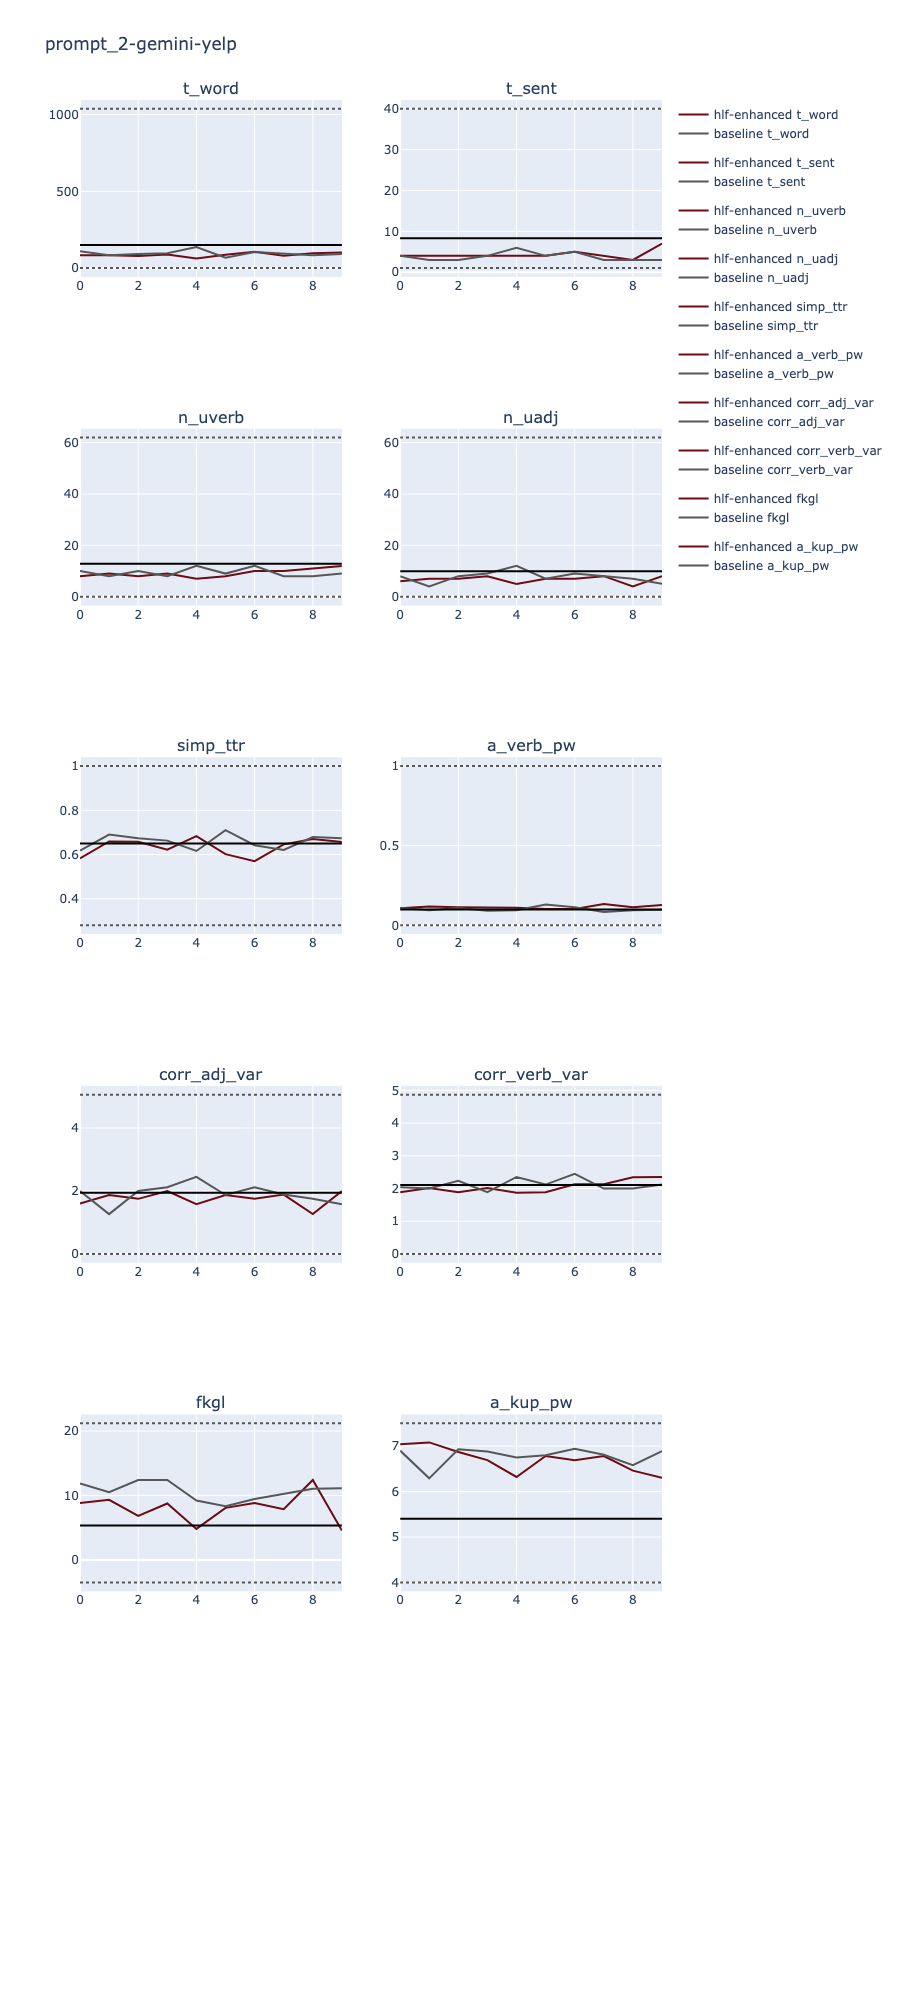
\includegraphics[width=\textwidth,height=0.9\textheight,scale=1]{plots/prompt_2/prompt_2-gemini-yelp/prompt_2-gemini-yelp.png}
    \caption{Gemini on Yelp Corpus\\Prompt With Examples\\Extraneous Input}\label{fig:gemini-prompt2-yelp}
\end{figure*}
\begin{figure*}[ht]
    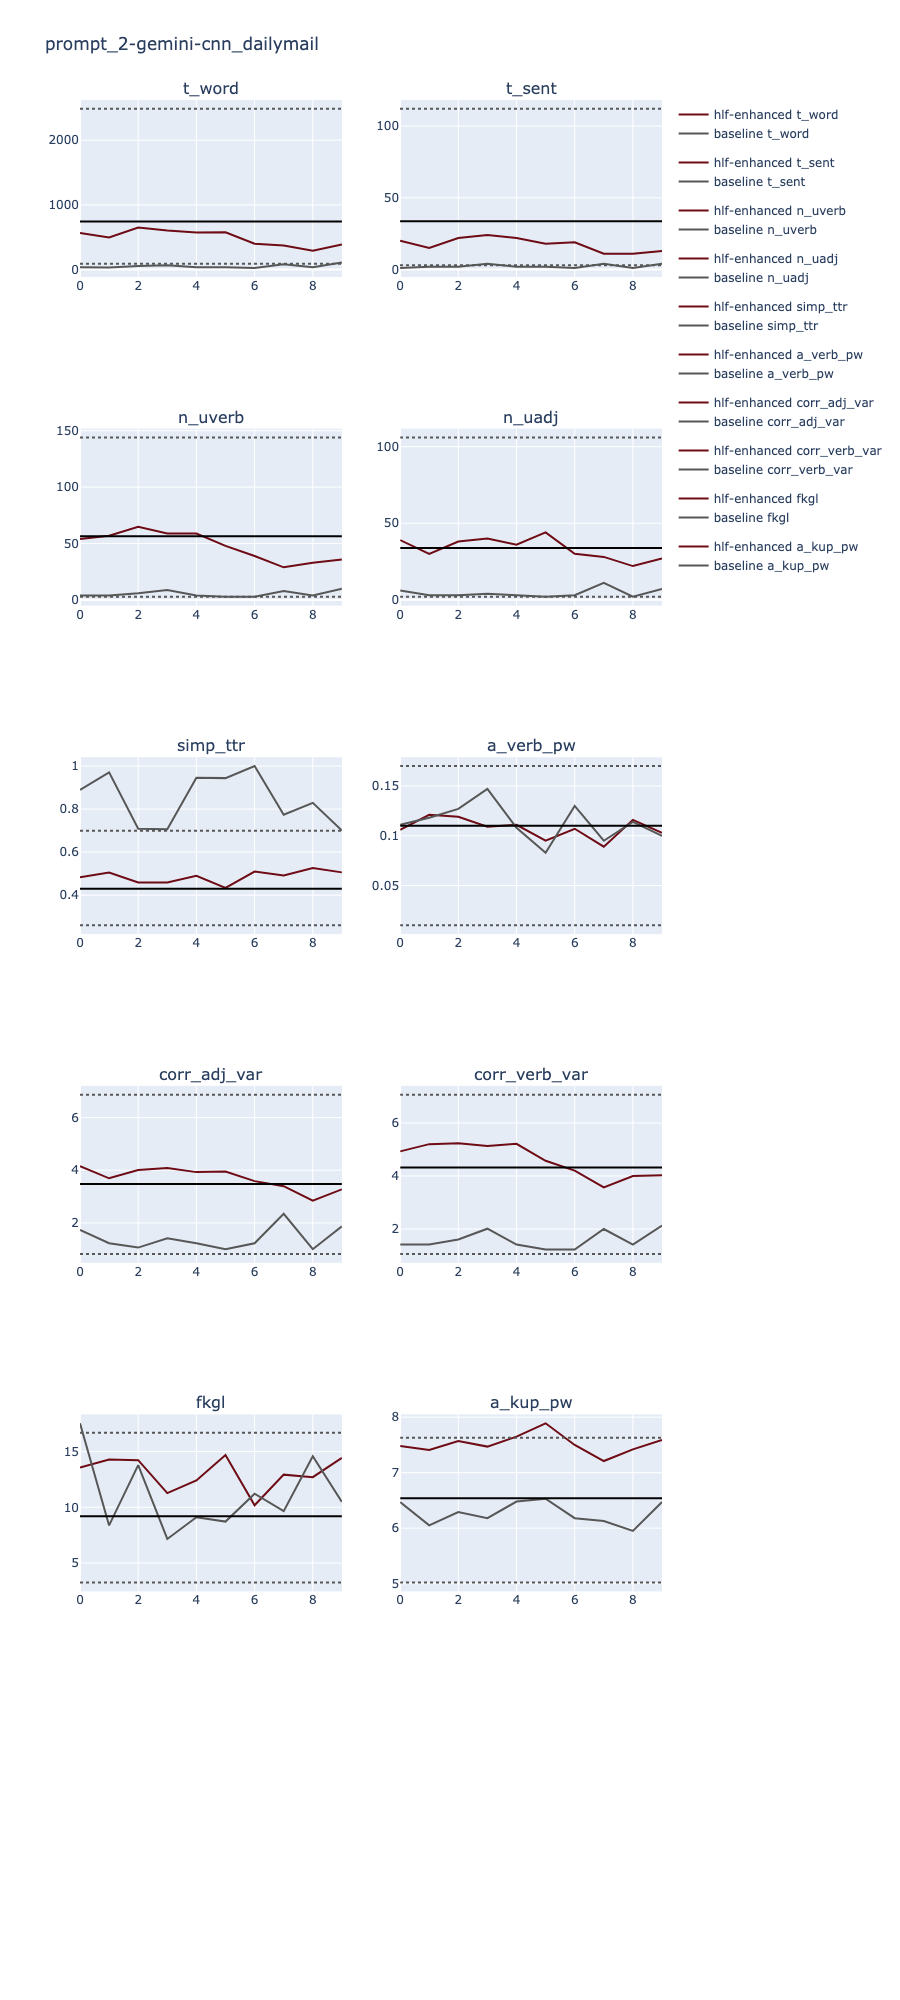
\includegraphics[width=\textwidth,height=0.9\textheight,scale=1]{plots/prompt_2_ifd/prompt_2-gemini-cnn_dailymail/prompt_2-gemini-cnn_dailymail.png}
    \caption{Gemini on CNN Corpus\\Prompt With Examples\\Input from Corpus}\label{fig:gemini-prompt2-cnn-ifd}
\end{figure*}
\begin{figure*}[ht]
    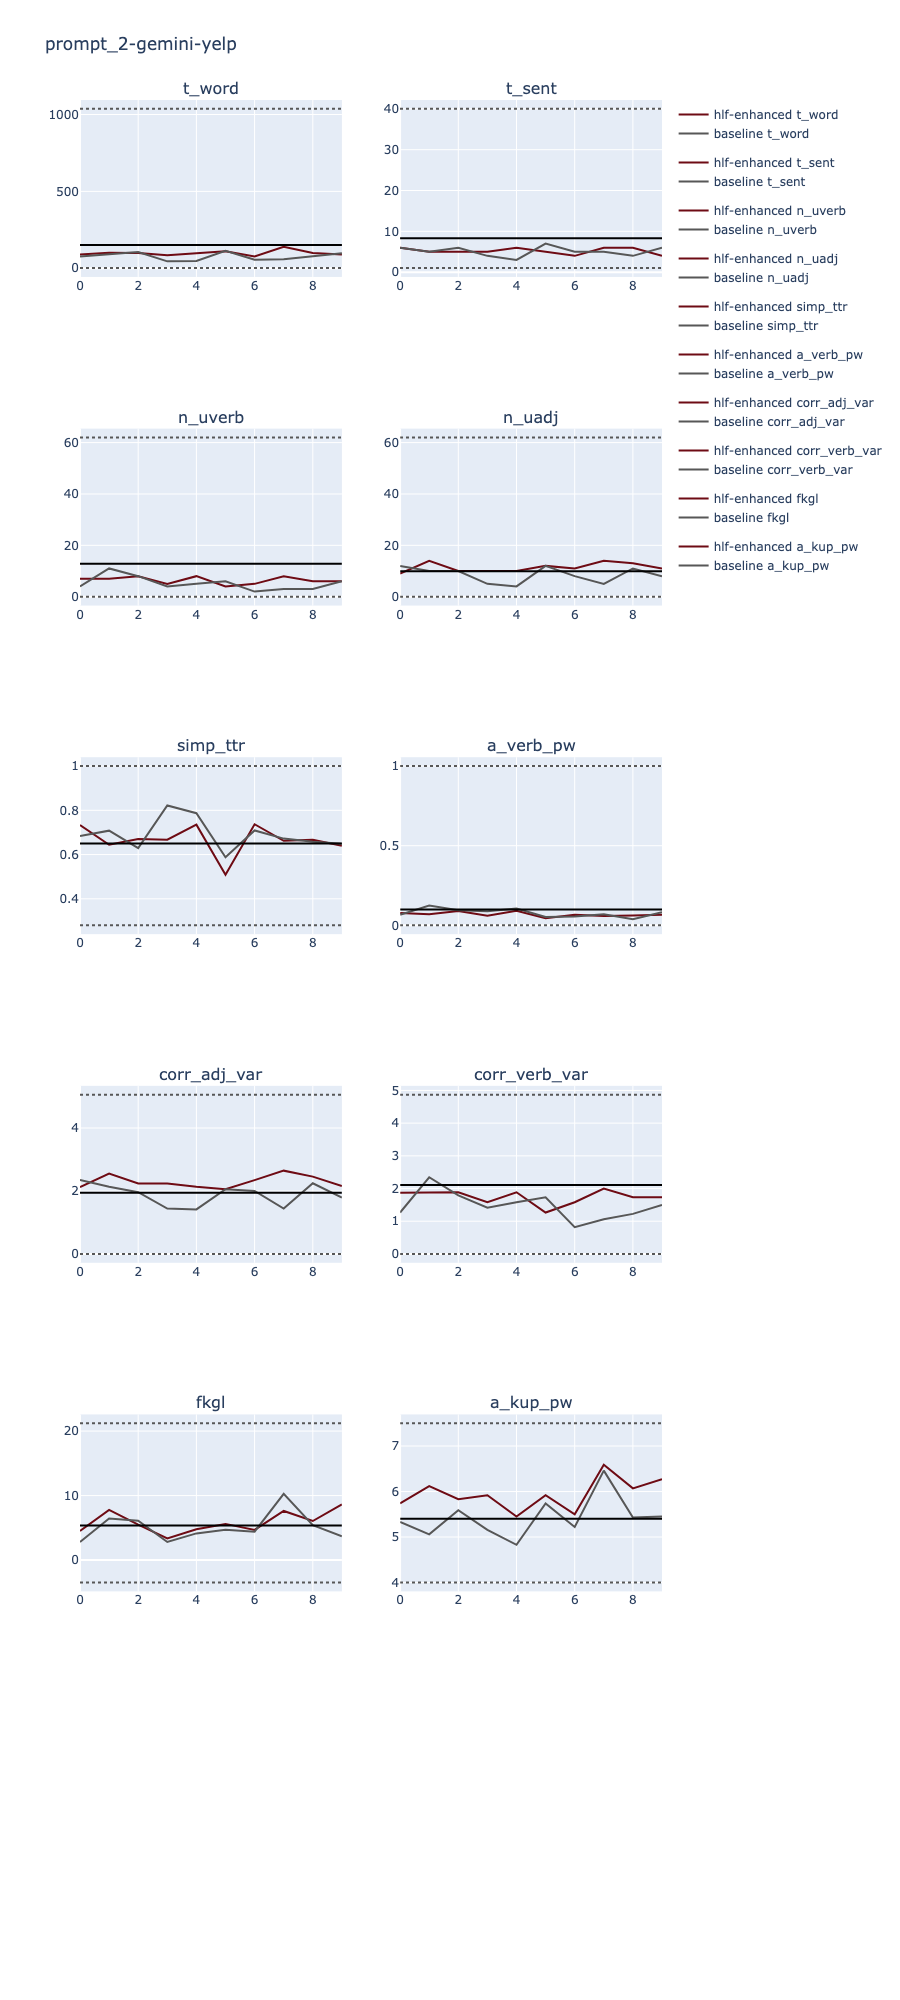
\includegraphics[width=\textwidth,height=0.9\textheight,scale=1]{plots/prompt_2_ifd/prompt_2-gemini-yelp/prompt_2-gemini-yelp.png}
    \caption{Gemini on Yelp Corpus\\Prompt With Examples\\Input from Corpus}\label{fig:gemini-prompt2-yelp-ifd}
\end{figure*}

\Cref{fig:gemini-prompt1-cnn,fig:gemini-prompt1-yelp,fig:gemini-prompt2-cnn,fig:gemini-prompt2-yelp,fig:gemini-prompt2-cnn-ifd,fig:gemini-prompt2-yelp-ifd}
show the experiment results for the Claude 3 Opus large language model.

\subsection{Claude3}

\begin{figure*}[ht]
    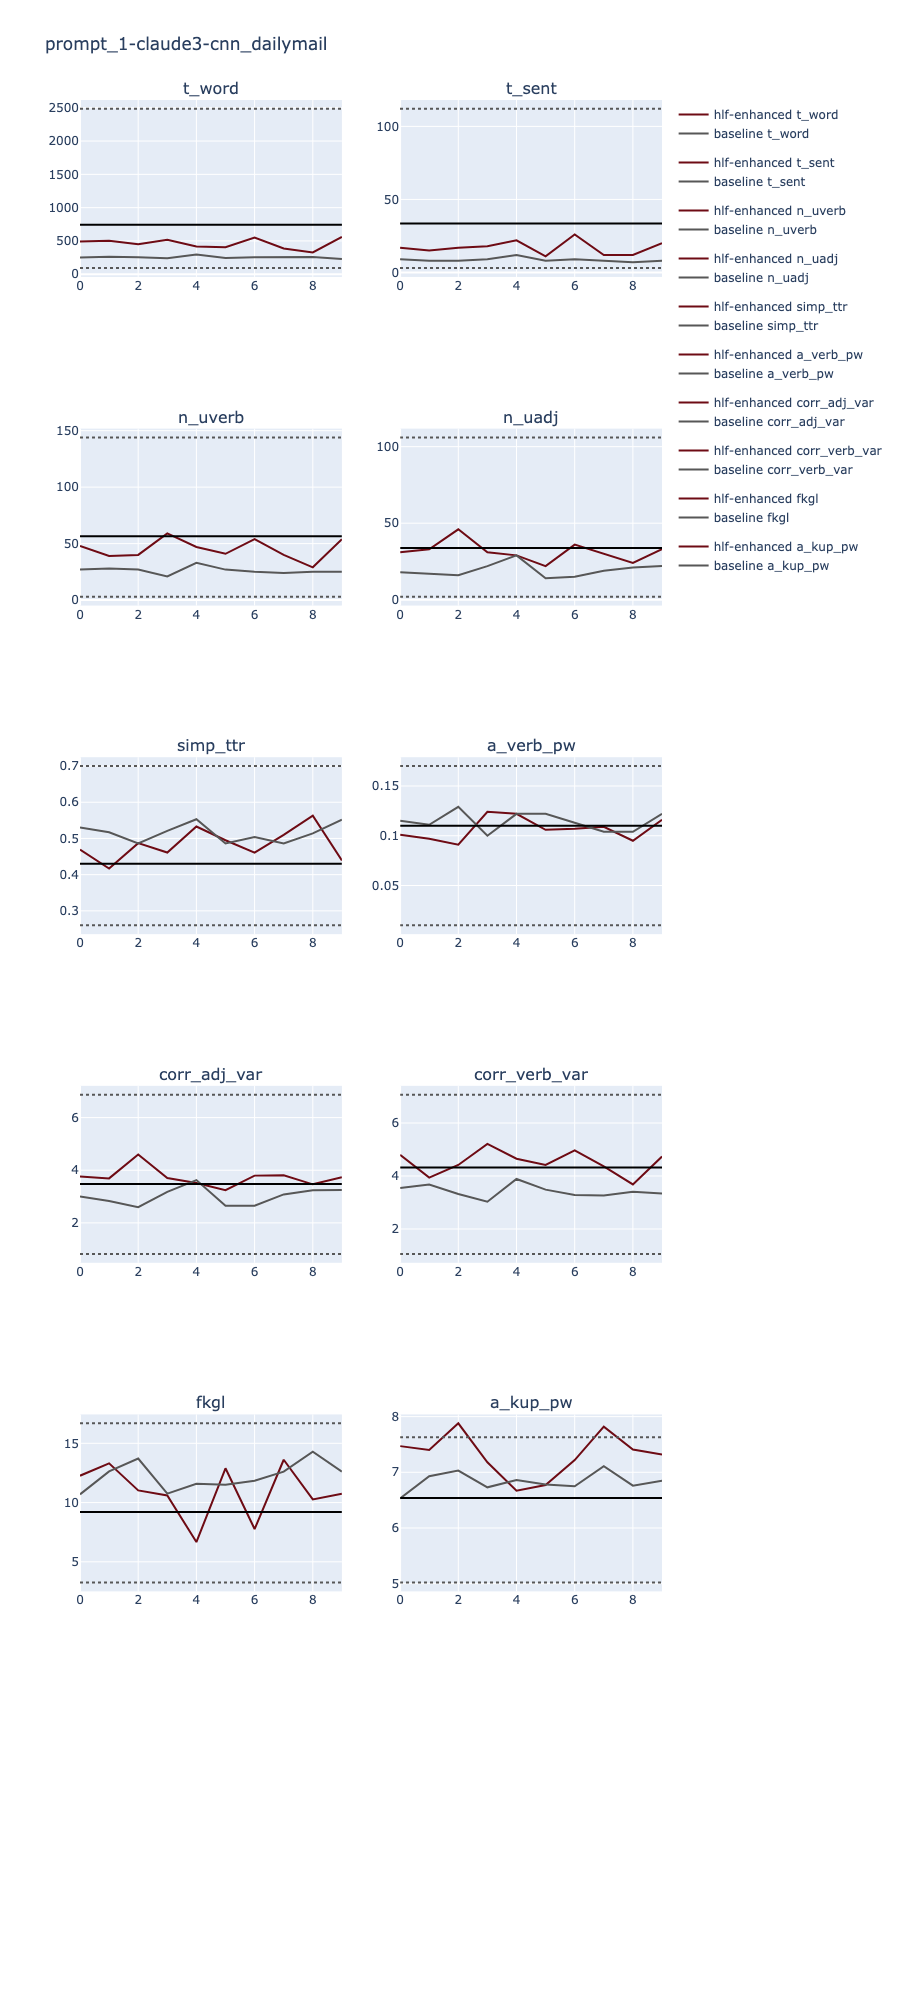
\includegraphics[width=\textwidth,height=0.9\textheight,scale=1]{plots/prompt_1/prompt_1-claude3-cnn_dailymail/prompt_1-claude3-cnn_dailymail.png}
    \caption{Claude3 on CNN Corpus\\Prompt Without Examples}\label{fig:claude3-prompt1-cnn}
\end{figure*}
\begin{figure*}[ht]
    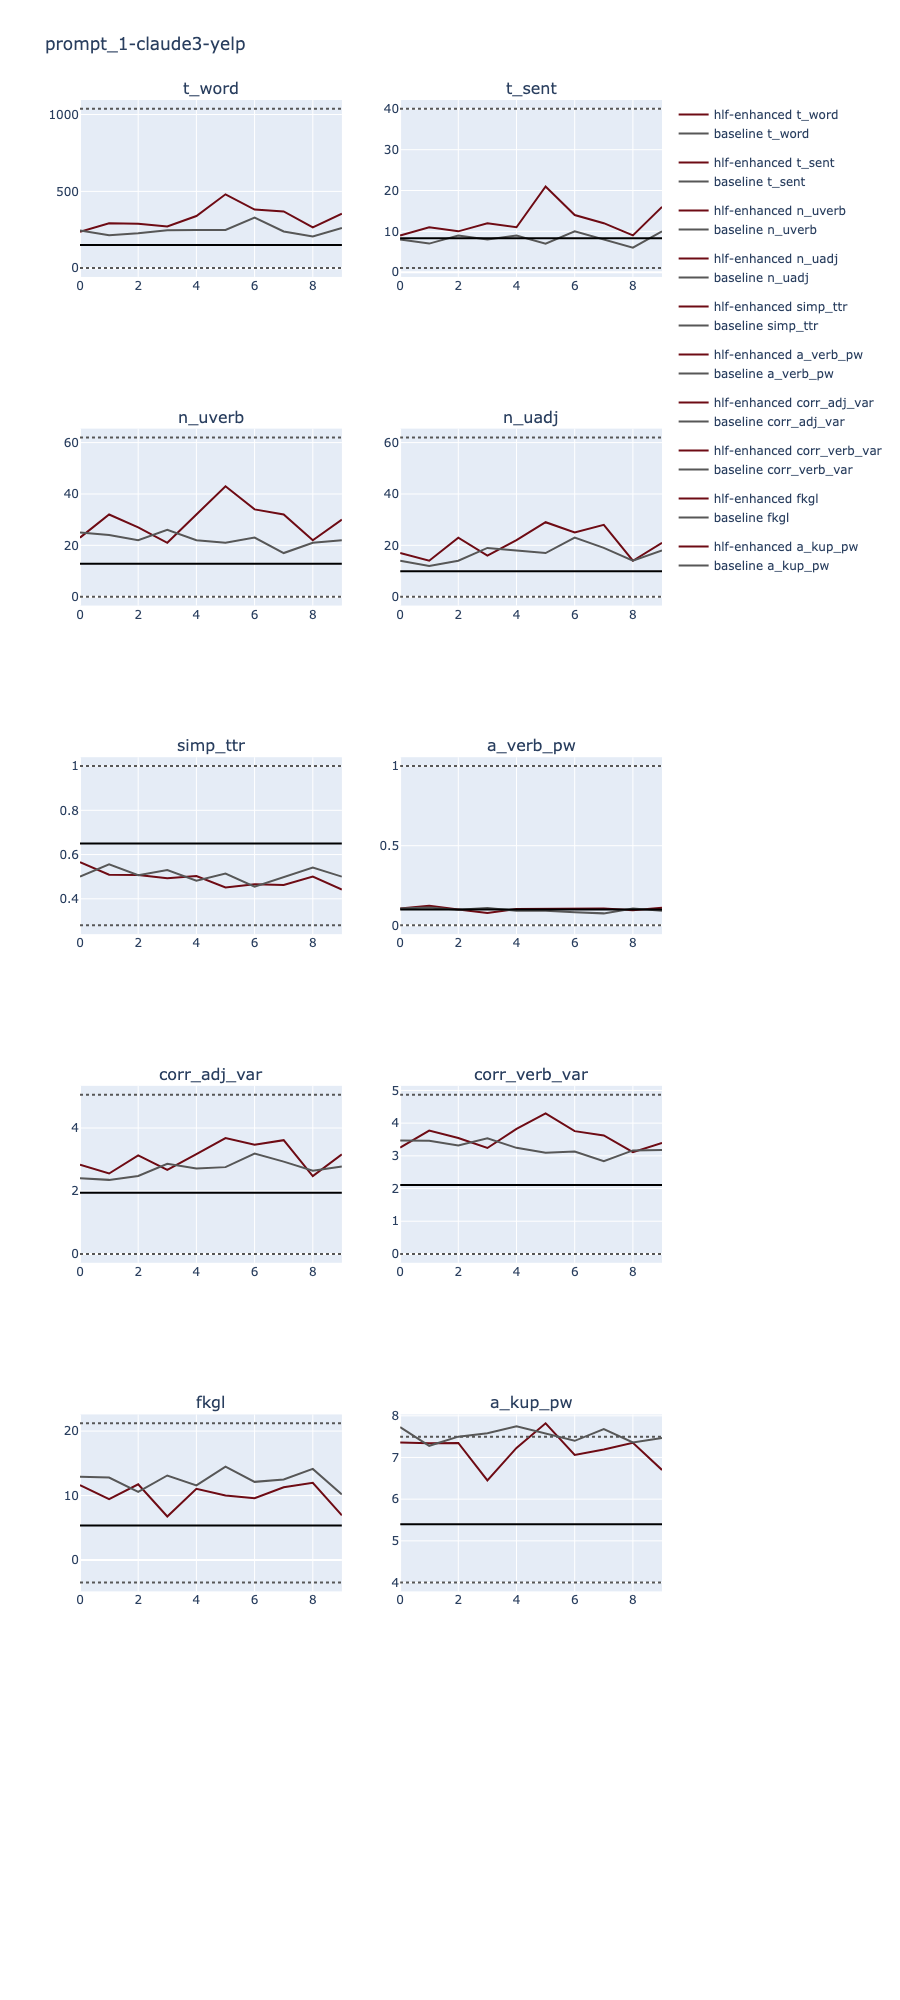
\includegraphics[width=\textwidth,height=0.9\textheight,scale=1]{plots/prompt_1/prompt_1-claude3-yelp/prompt_1-claude3-yelp.png}
    \caption{Claude3 on Yelp Corpus\\Prompt Without Examples}\label{fig:claude3-prompt1-yelp}
\end{figure*}
\begin{figure*}[ht]
    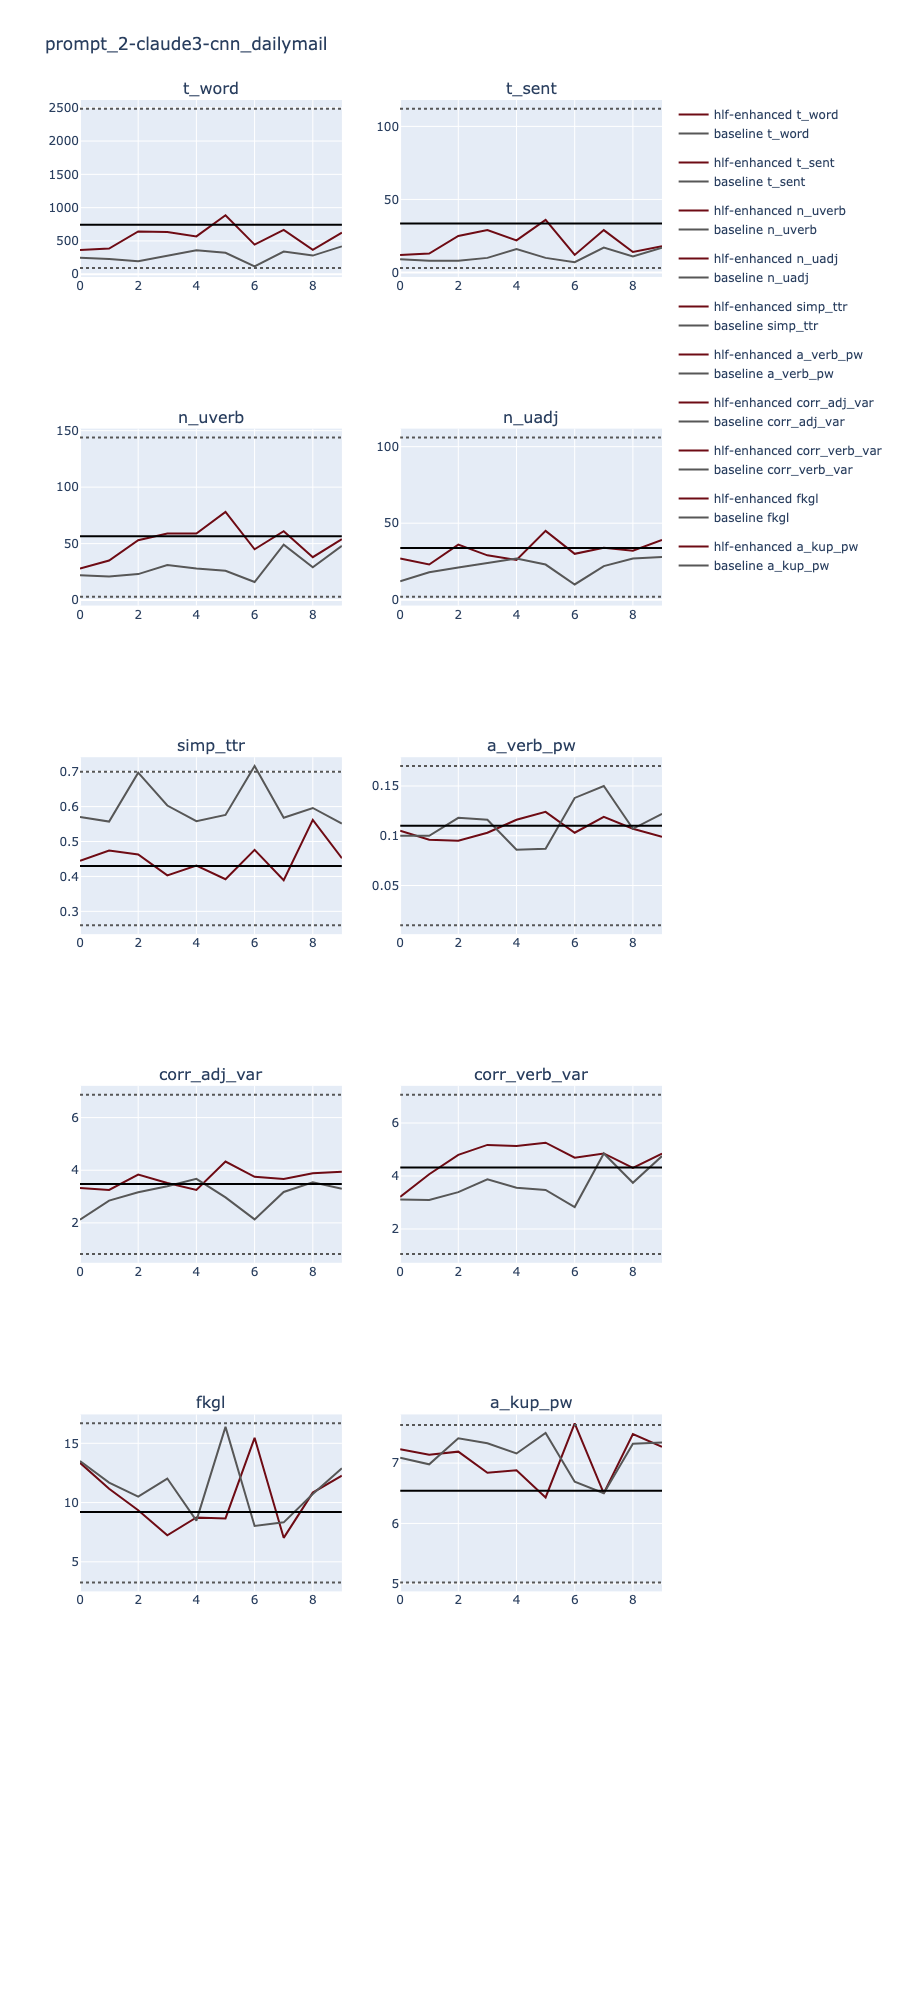
\includegraphics[width=\textwidth,height=0.9\textheight,scale=1]{plots/prompt_2/prompt_2-claude3-cnn_dailymail/prompt_2-claude3-cnn_dailymail.png}
    \caption{Claude3 on CNN Corpus\\Prompt With Examples\\Extraneous Input}\label{fig:claude3-prompt2-cnn}
\end{figure*}
\begin{figure*}[ht]
    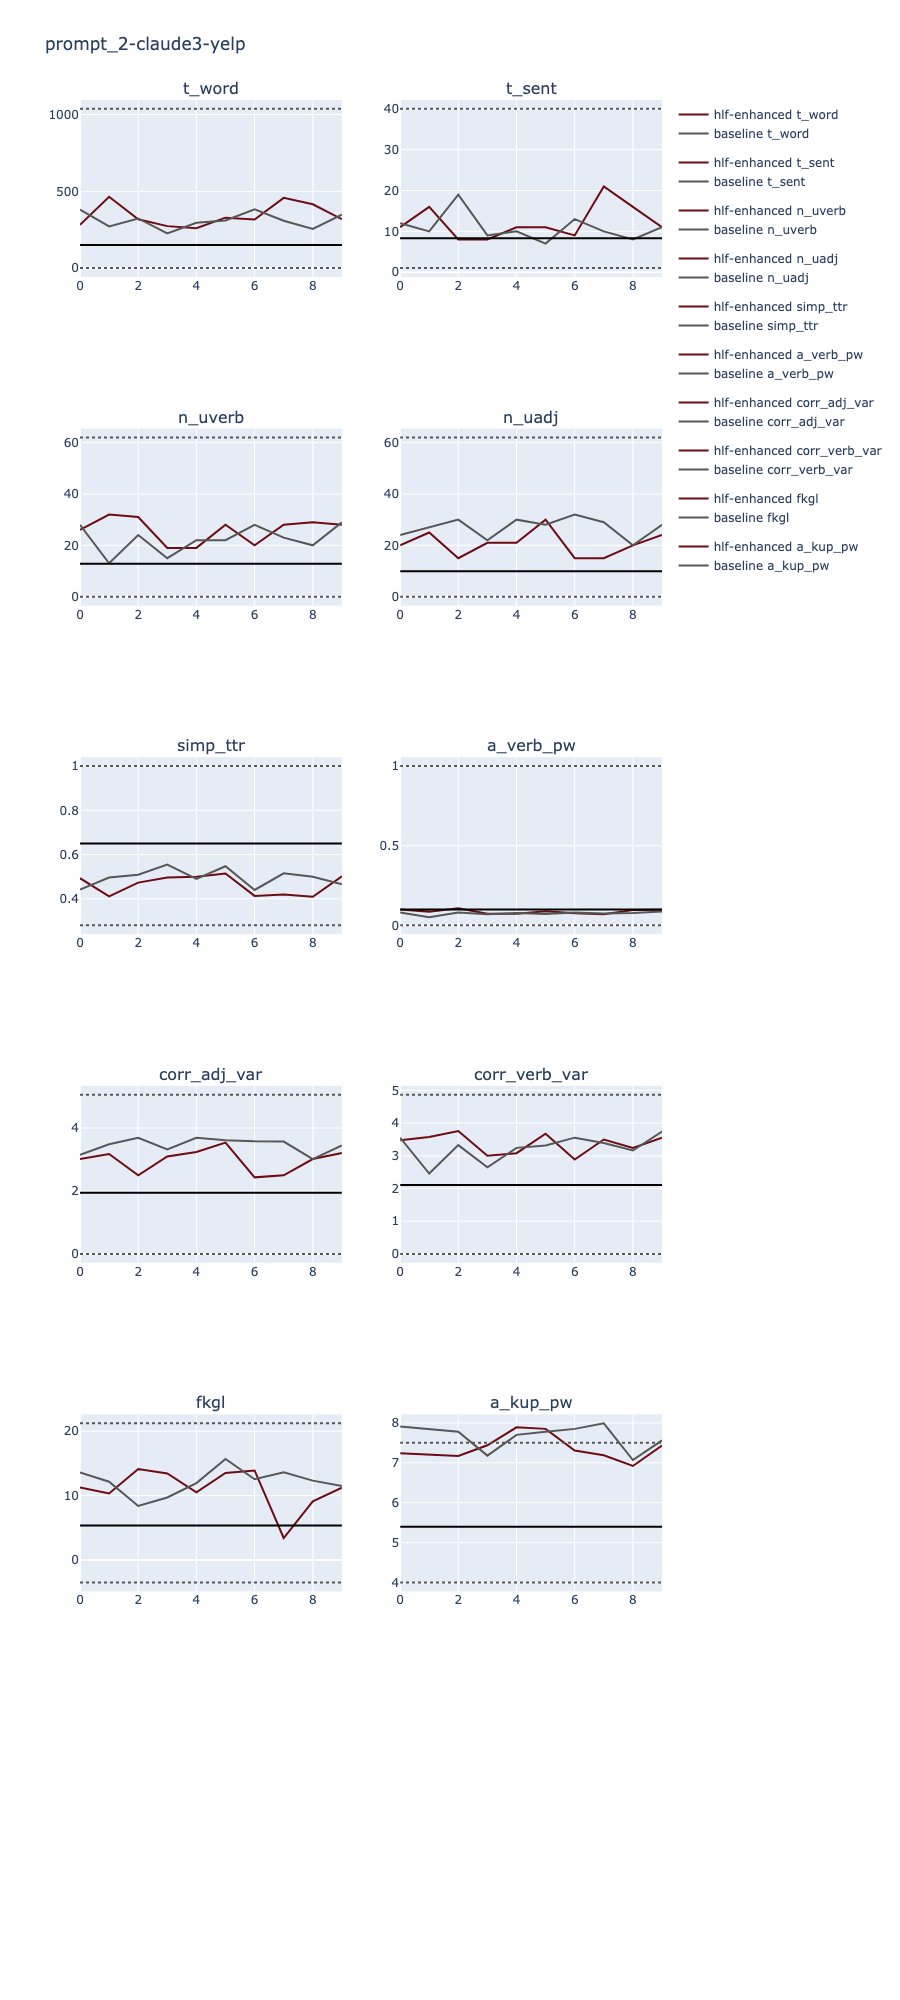
\includegraphics[width=\textwidth,height=0.9\textheight,scale=1]{plots/prompt_2/prompt_2-claude3-yelp/prompt_2-claude3-yelp.png}
    \caption{Claude3 on Yelp Corpus\\Prompt With Examples\\Extraneous Input}\label{fig:claude3-prompt2-yelp}
\end{figure*}
\begin{figure*}[ht]
    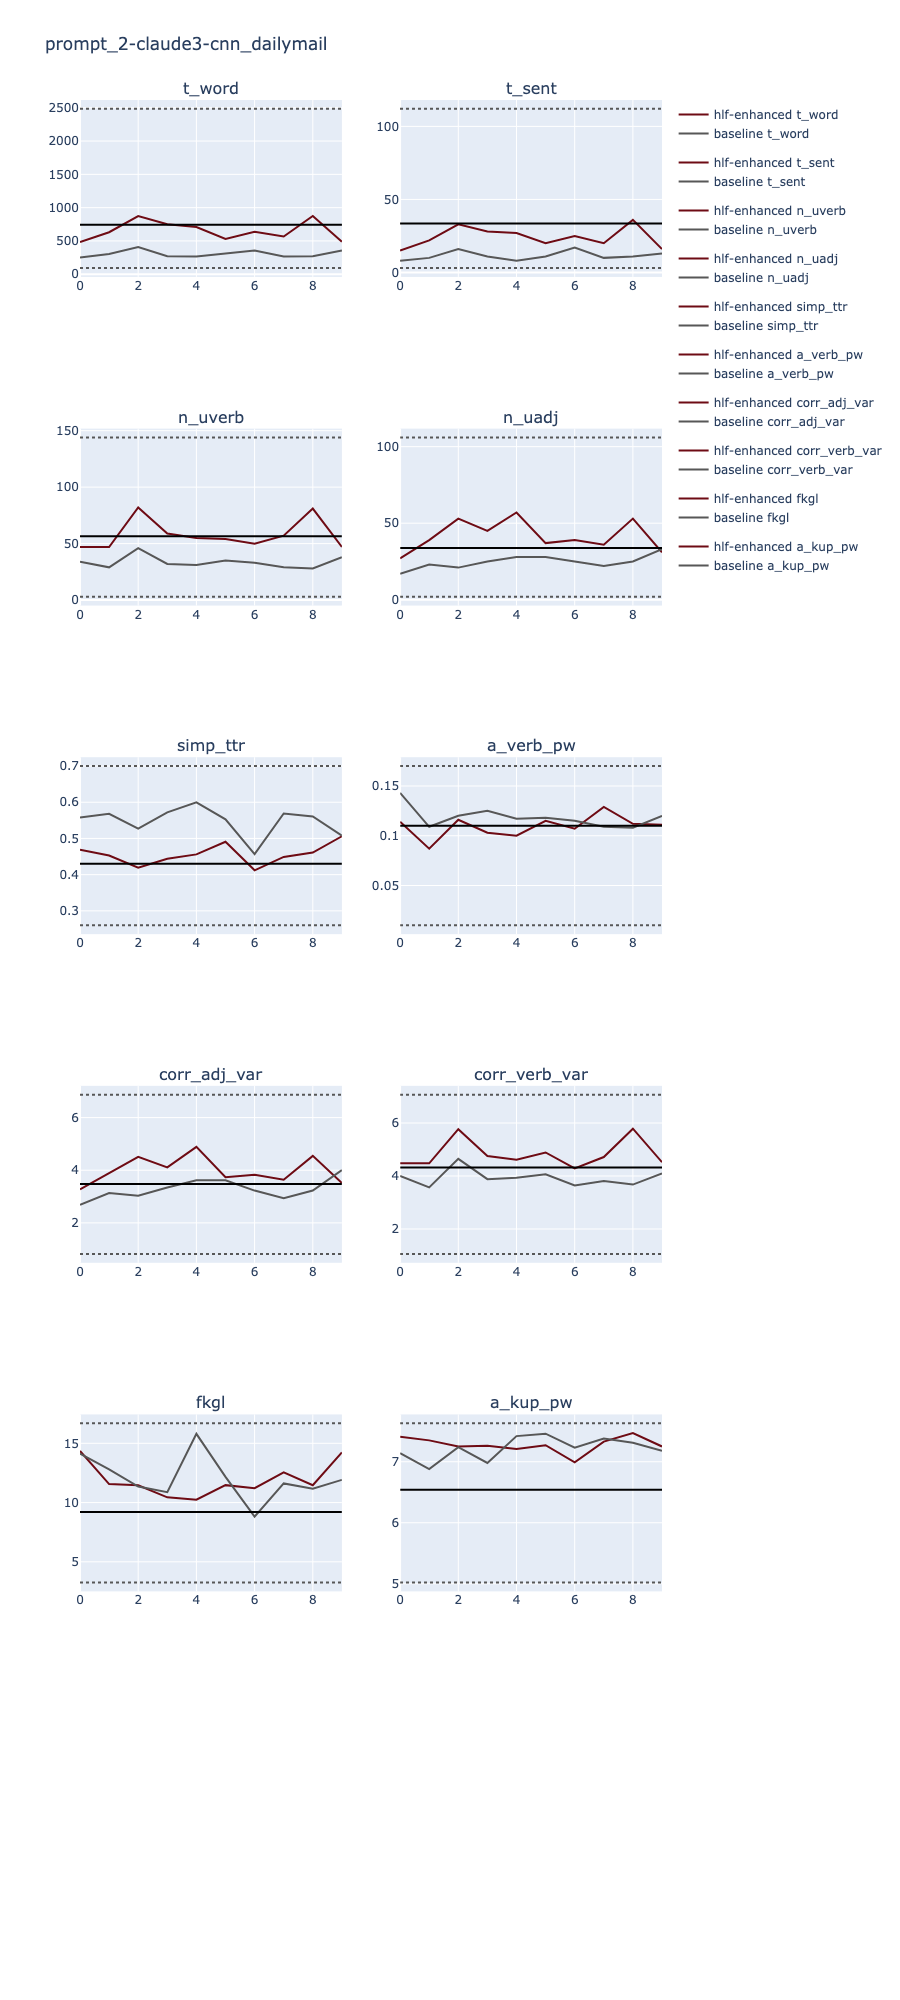
\includegraphics[width=\textwidth,height=0.9\textheight,scale=1]{plots/prompt_2_ifd/prompt_2-claude3-cnn_dailymail/prompt_2-claude3-cnn_dailymail.png}
    \caption{Claude3 on CNN Corpus\\Prompt With Examples\\Input from Corpus}\label{fig:claude3-prompt2-cnn-ifd}
\end{figure*}
\begin{figure*}[ht]
    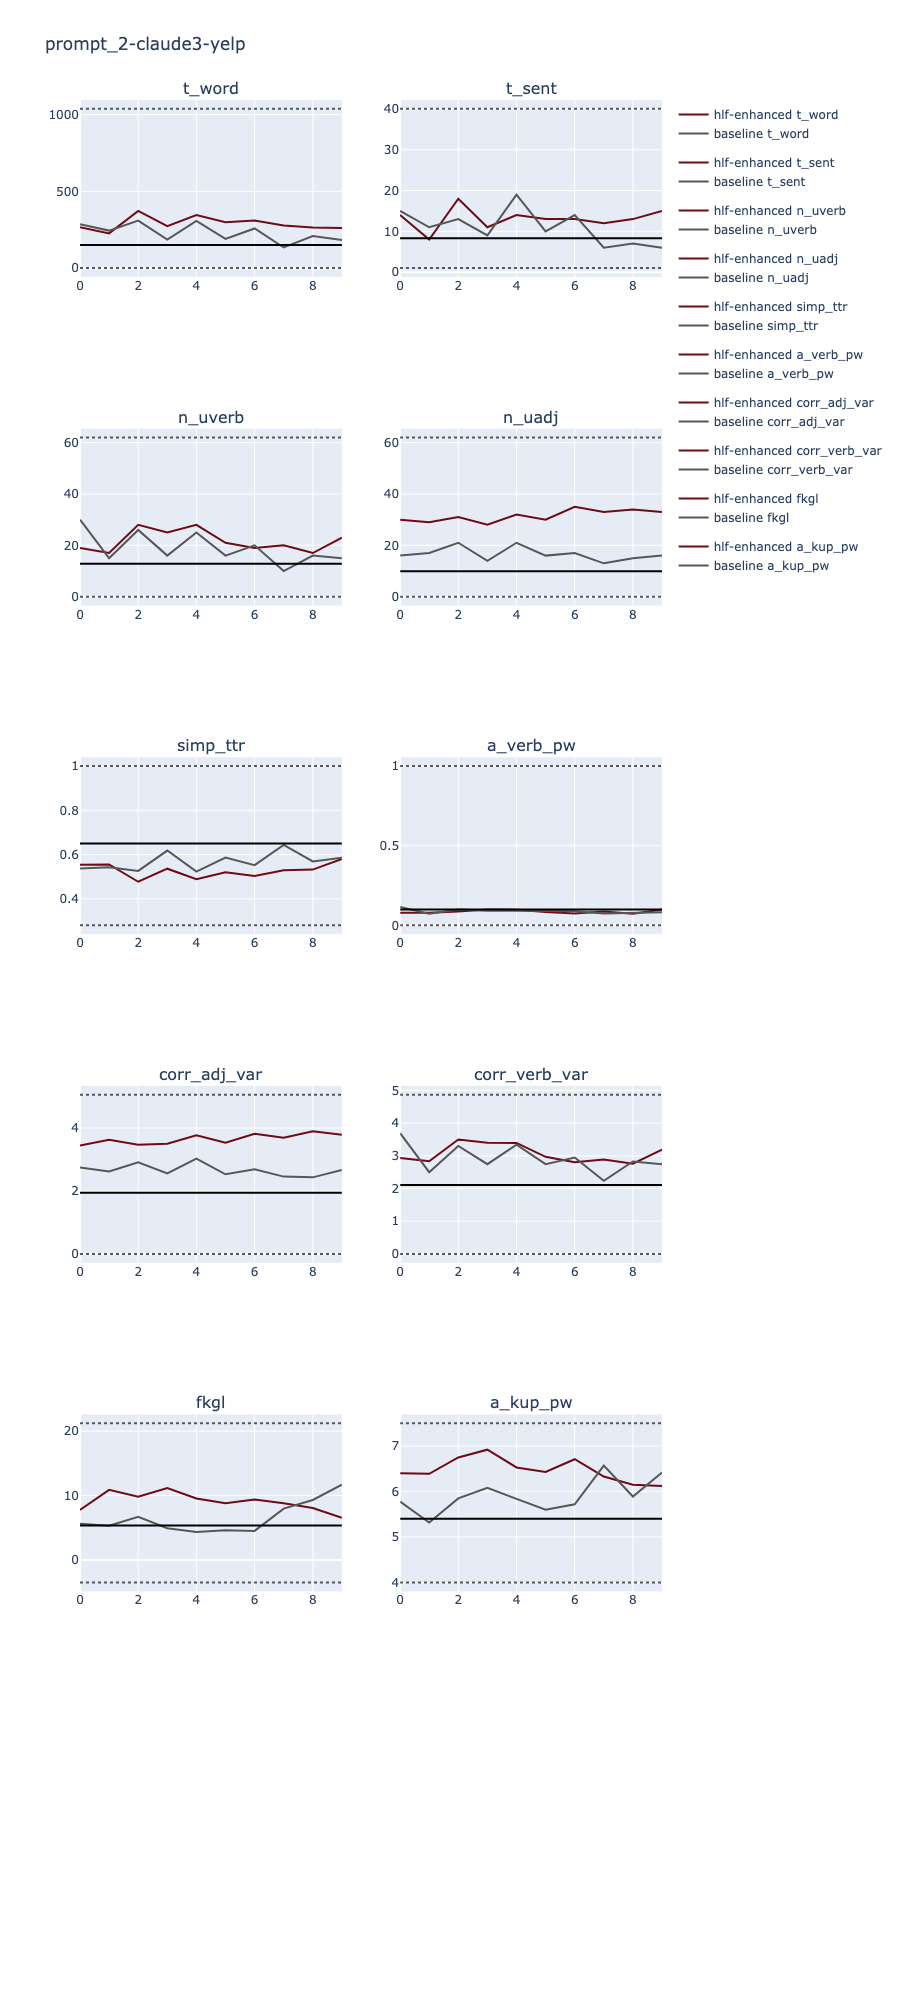
\includegraphics[width=\textwidth,height=0.9\textheight,scale=1]{plots/prompt_2_ifd/prompt_2-claude3-yelp/prompt_2-claude3-yelp.png}
    \caption{Claude3 on Yelp Corpus\\Prompt With Examples\\Input from Corpus}\label{fig:claude3-prompt2-yelp-ifd}
\end{figure*}

\Cref{fig:claude3-prompt1-cnn,fig:claude3-prompt1-yelp,fig:claude3-prompt2-cnn,fig:claude3-prompt2-yelp,fig:claude3-prompt2-cnn-ifd,fig:claude3-prompt2-yelp-ifd}
show the experiment results for the Claude 3 Opus large language model.

\subsection{Llama3}

\begin{figure*}[ht]
    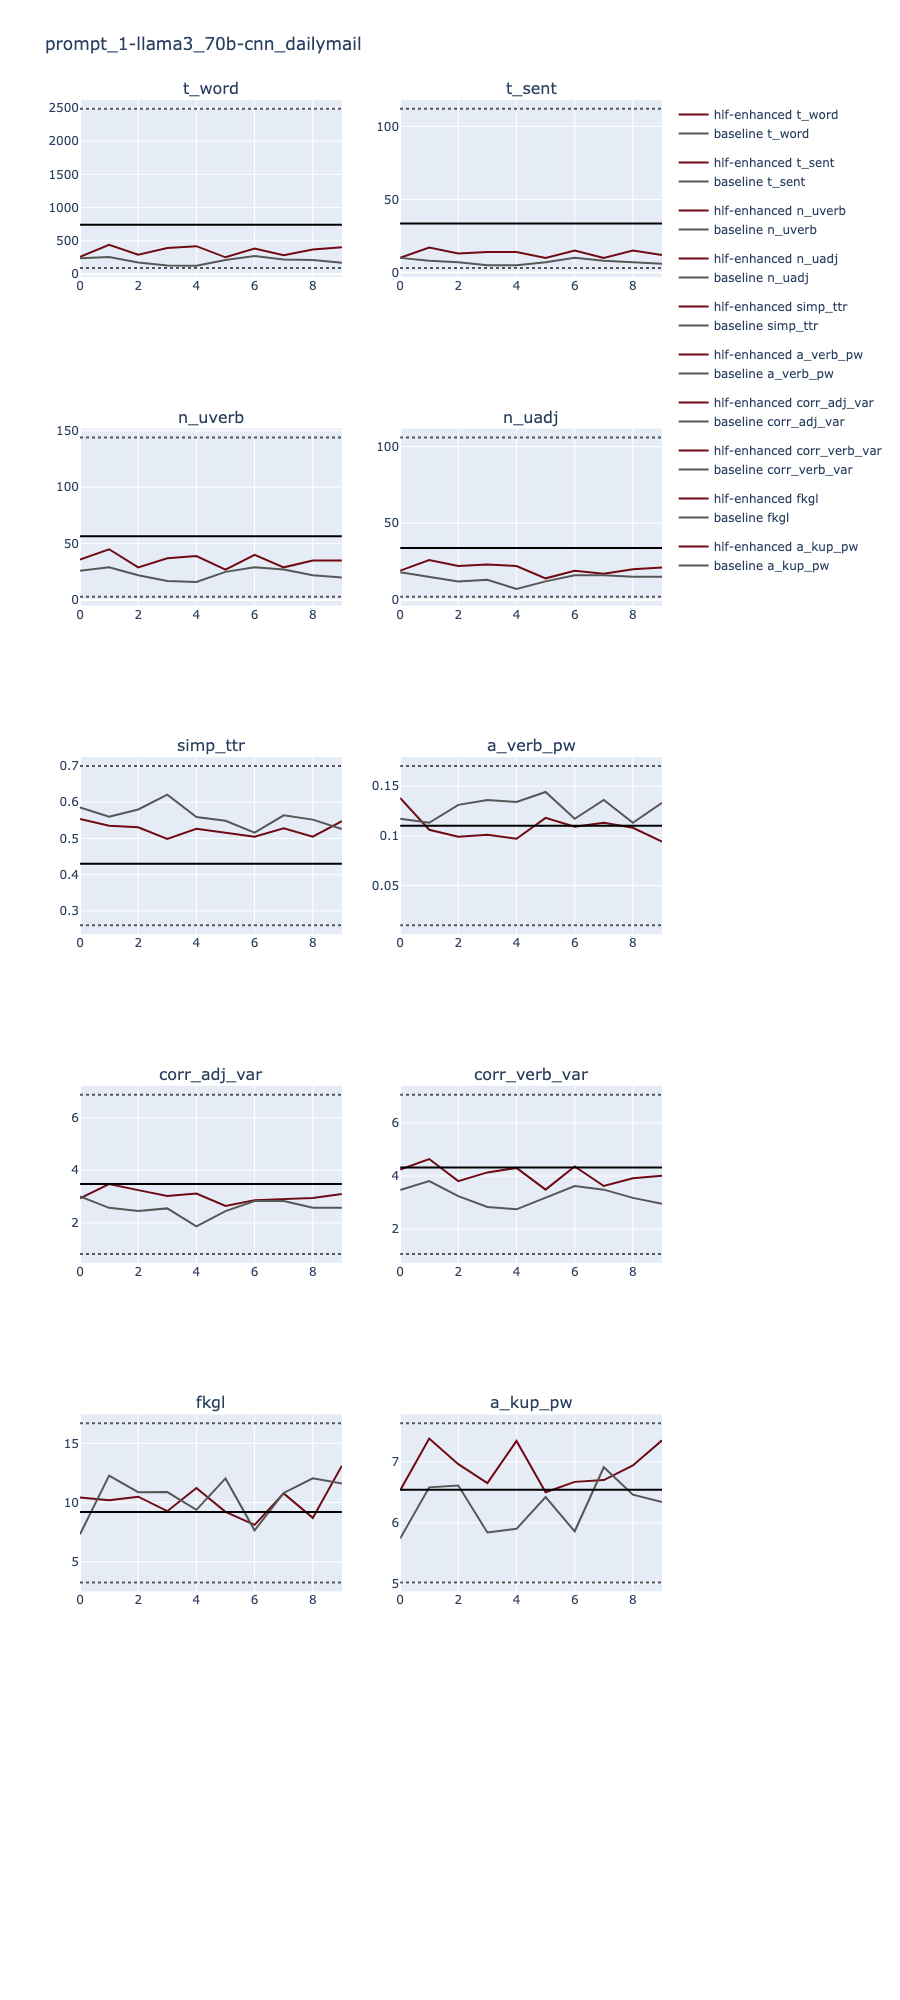
\includegraphics[width=\textwidth,height=0.9\textheight,scale=1]{plots/prompt_1/prompt_1-llama3_70b-cnn_dailymail/prompt_1-llama3_70b-cnn_dailymail.png}
    \caption{Llama3 on CNN Corpus\\Prompt Without Examples}\label{fig:llama3_70b-prompt1-cnn}
\end{figure*}
\begin{figure*}[ht]
    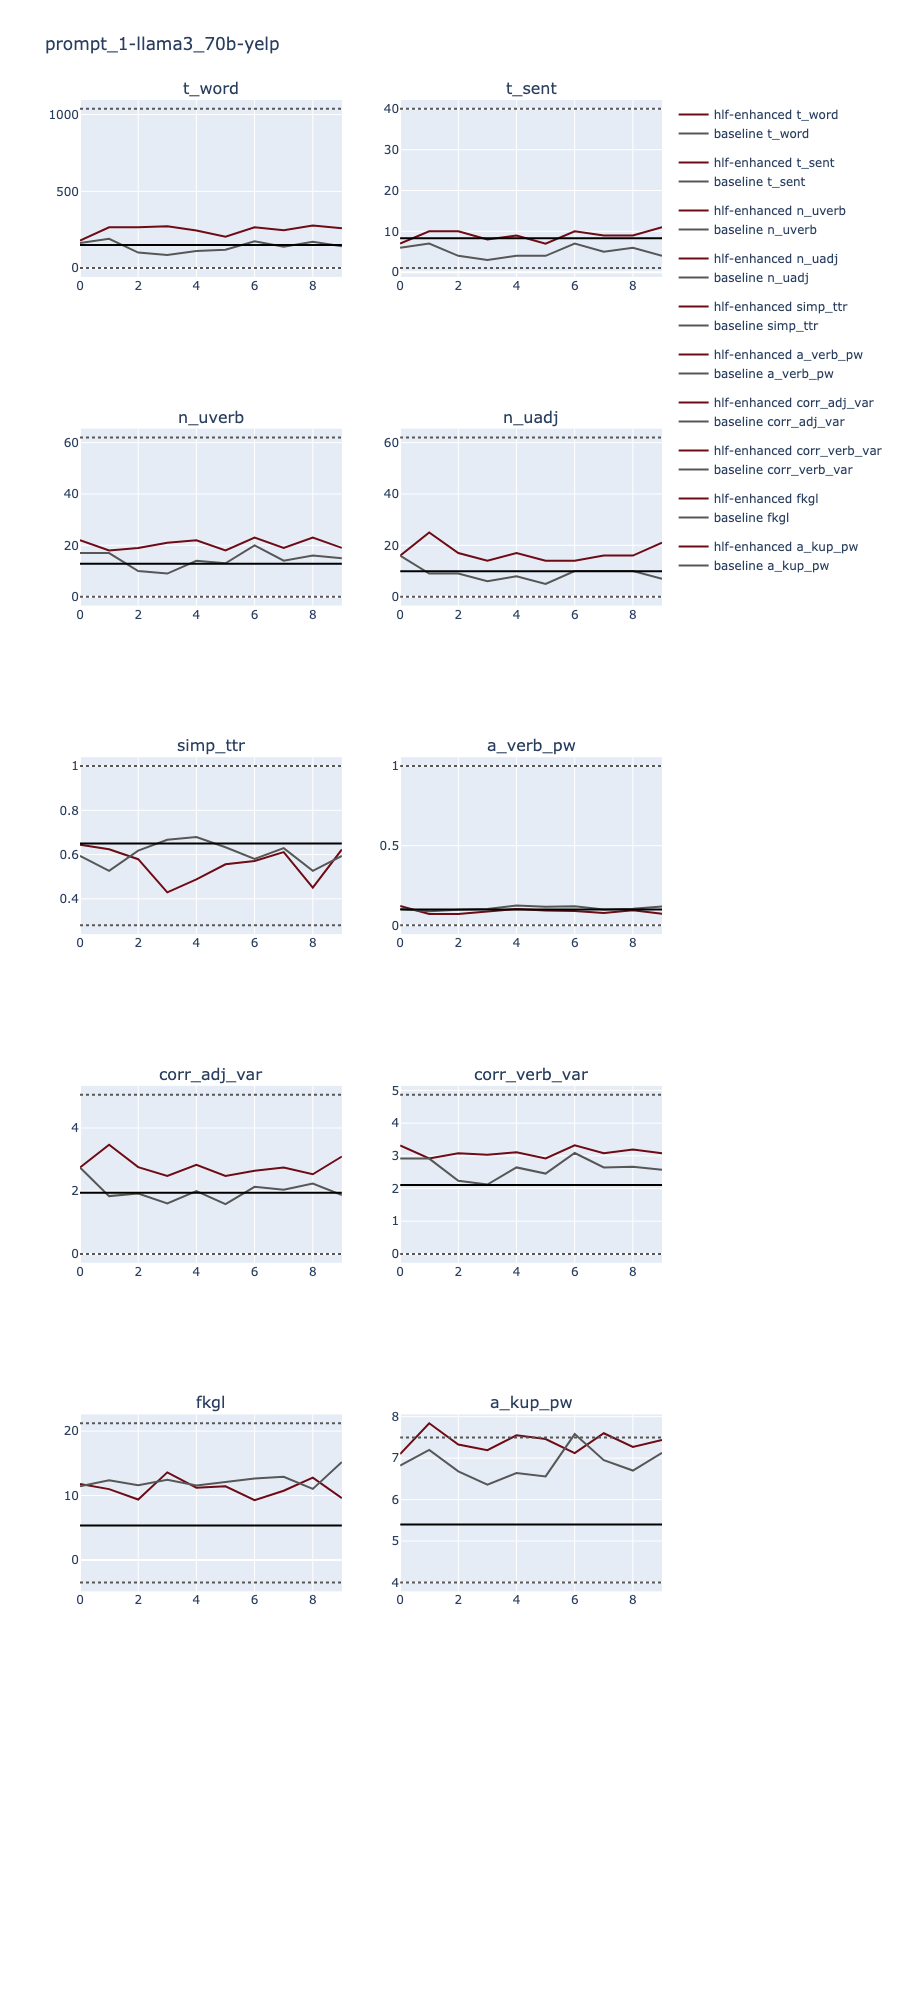
\includegraphics[width=\textwidth,height=0.9\textheight,scale=1]{plots/prompt_1/prompt_1-llama3_70b-yelp/prompt_1-llama3_70b-yelp.png}
    \caption{Llama3 on Yelp Corpus\\Prompt Without Examples}\label{fig:llama3_70b-prompt1-yelp}
\end{figure*}
\begin{figure*}[ht]
    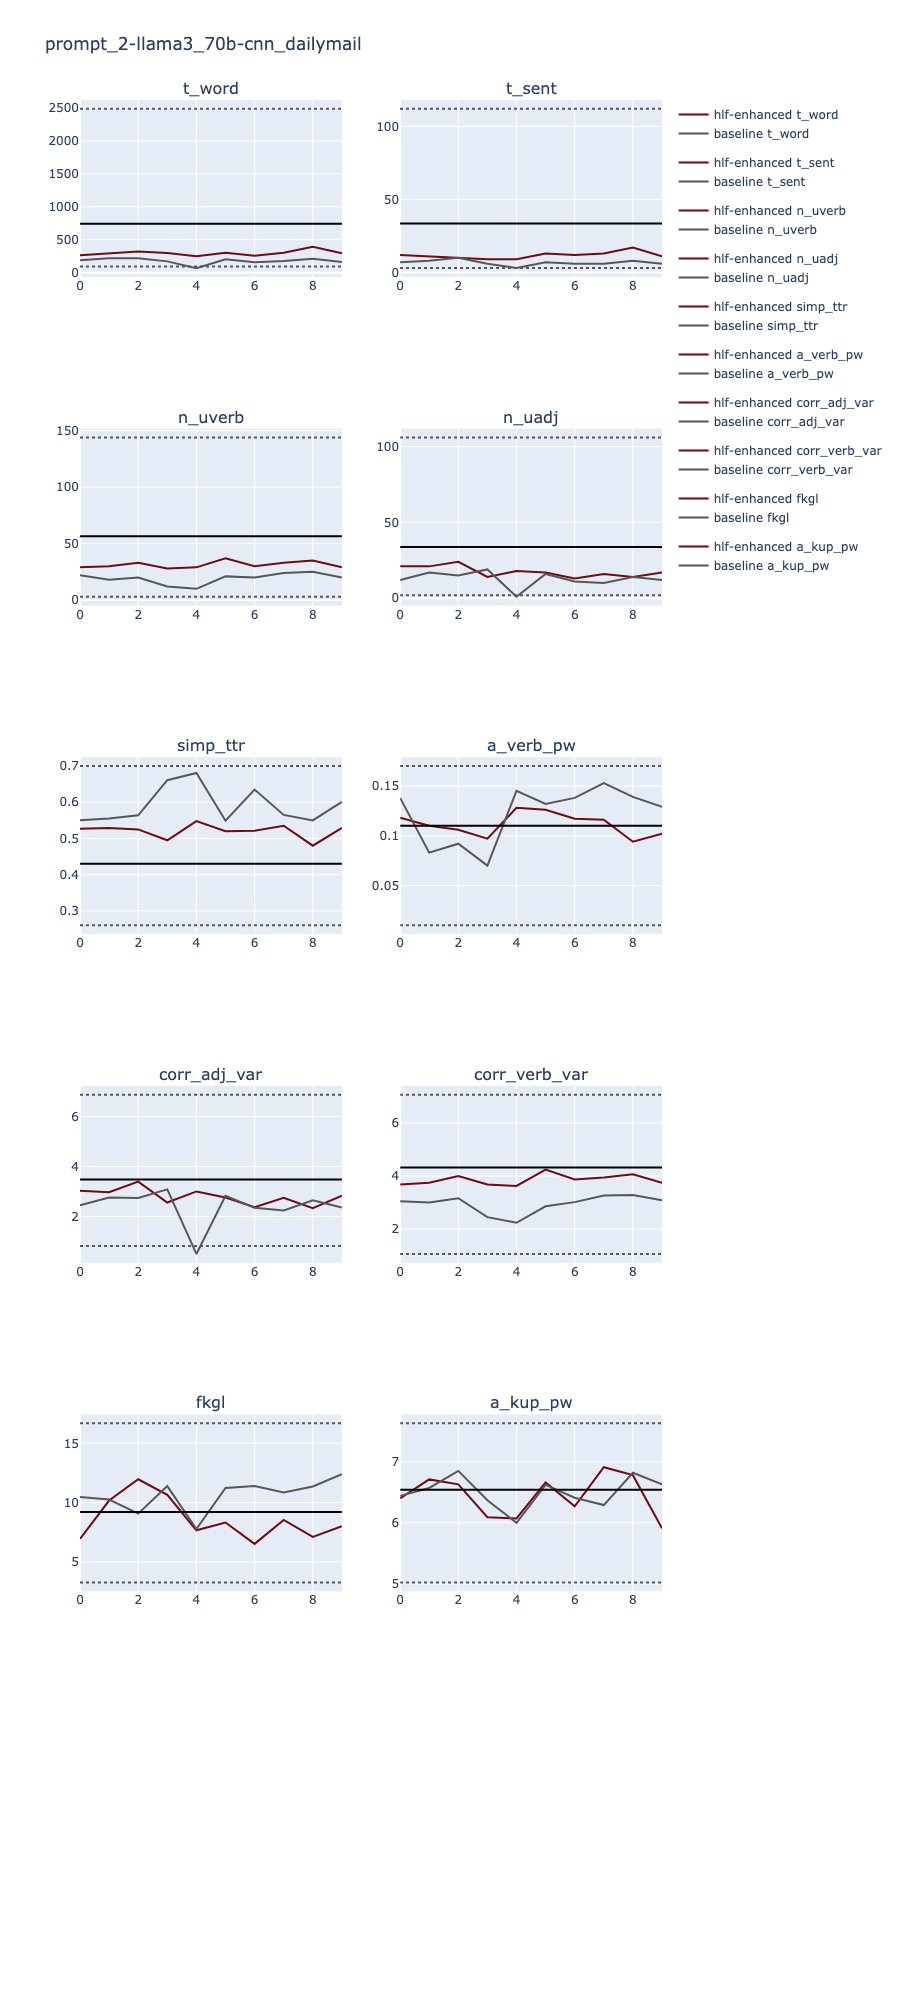
\includegraphics[width=\textwidth,height=0.9\textheight,scale=1]{plots/prompt_2/prompt_2-llama3_70b-cnn_dailymail/prompt_2-llama3_70b-cnn_dailymail.png}
    \caption{Llama3 on CNN Corpus\\Prompt With Examples\\Extraneous Input}\label{fig:llama3_70b-prompt2-cnn}
\end{figure*}
\begin{figure*}[ht]
    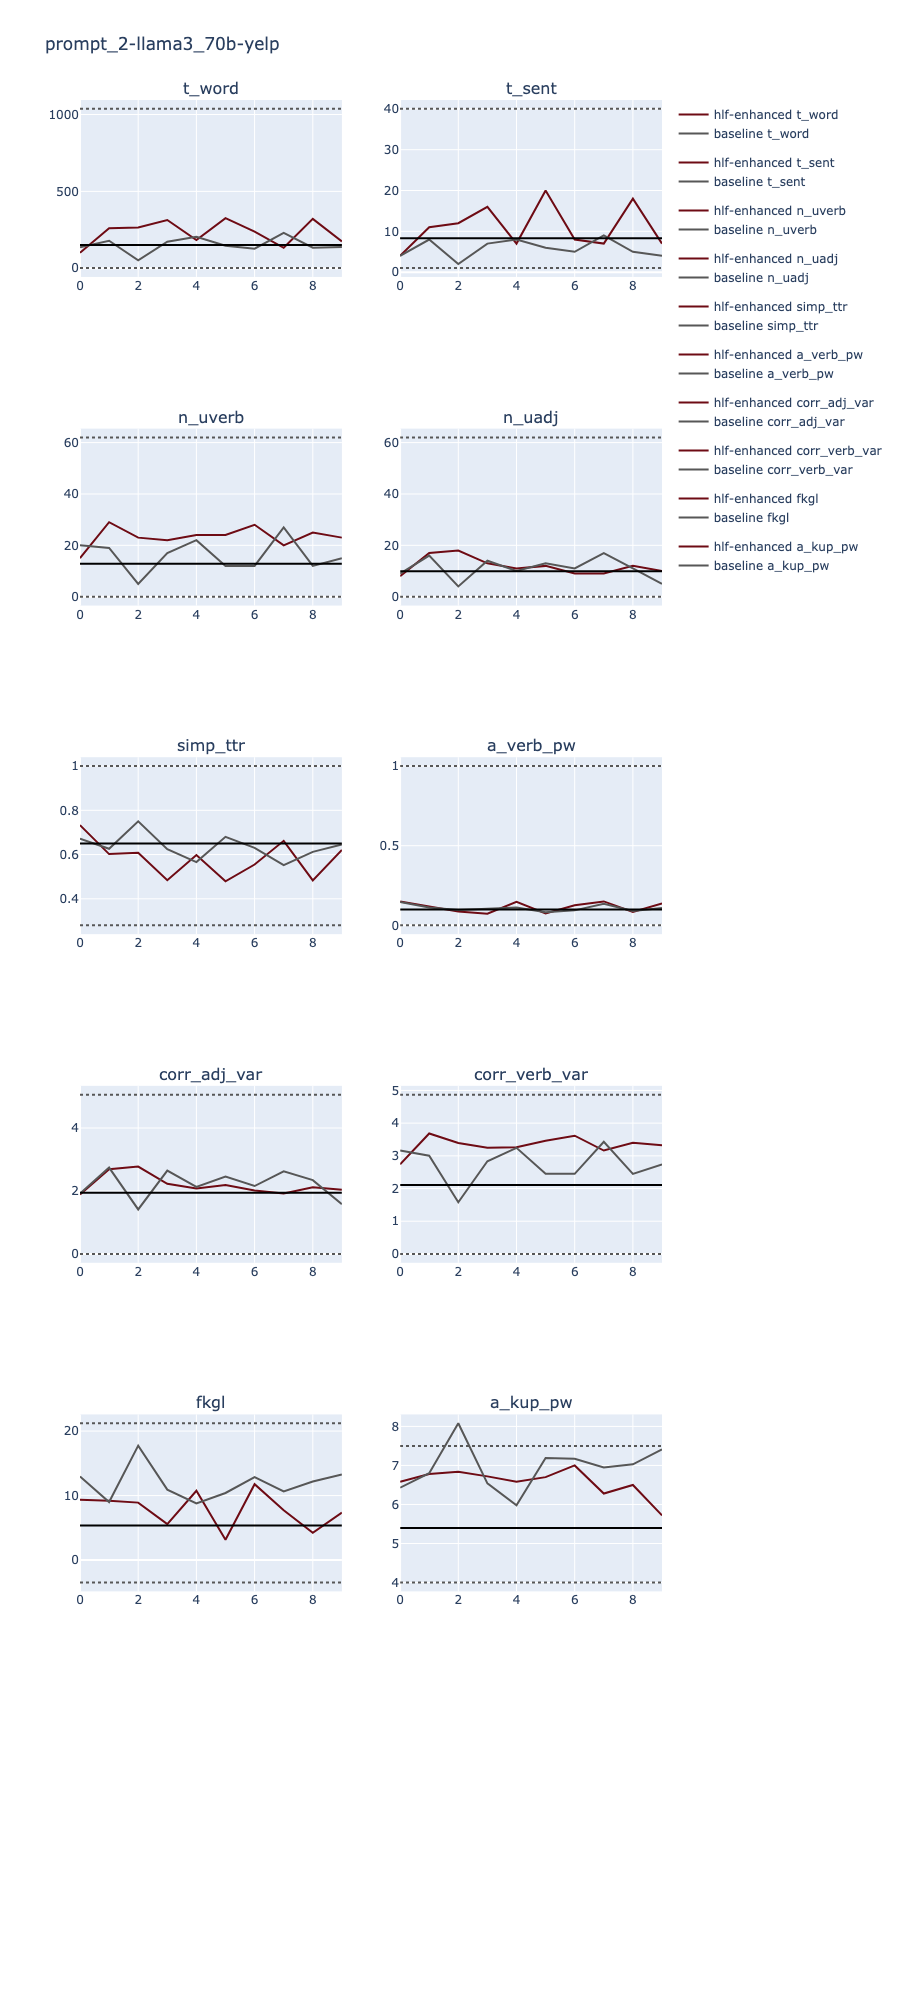
\includegraphics[width=\textwidth,height=0.9\textheight,scale=1]{plots/prompt_2/prompt_2-llama3_70b-yelp/prompt_2-llama3_70b-yelp.png}
    \caption{Llama3 on Yelp Corpus\\Prompt With Examples\\Extraneous Input}\label{fig:llama3_70b-prompt2-yelp}
\end{figure*}
\begin{figure*}[ht]
    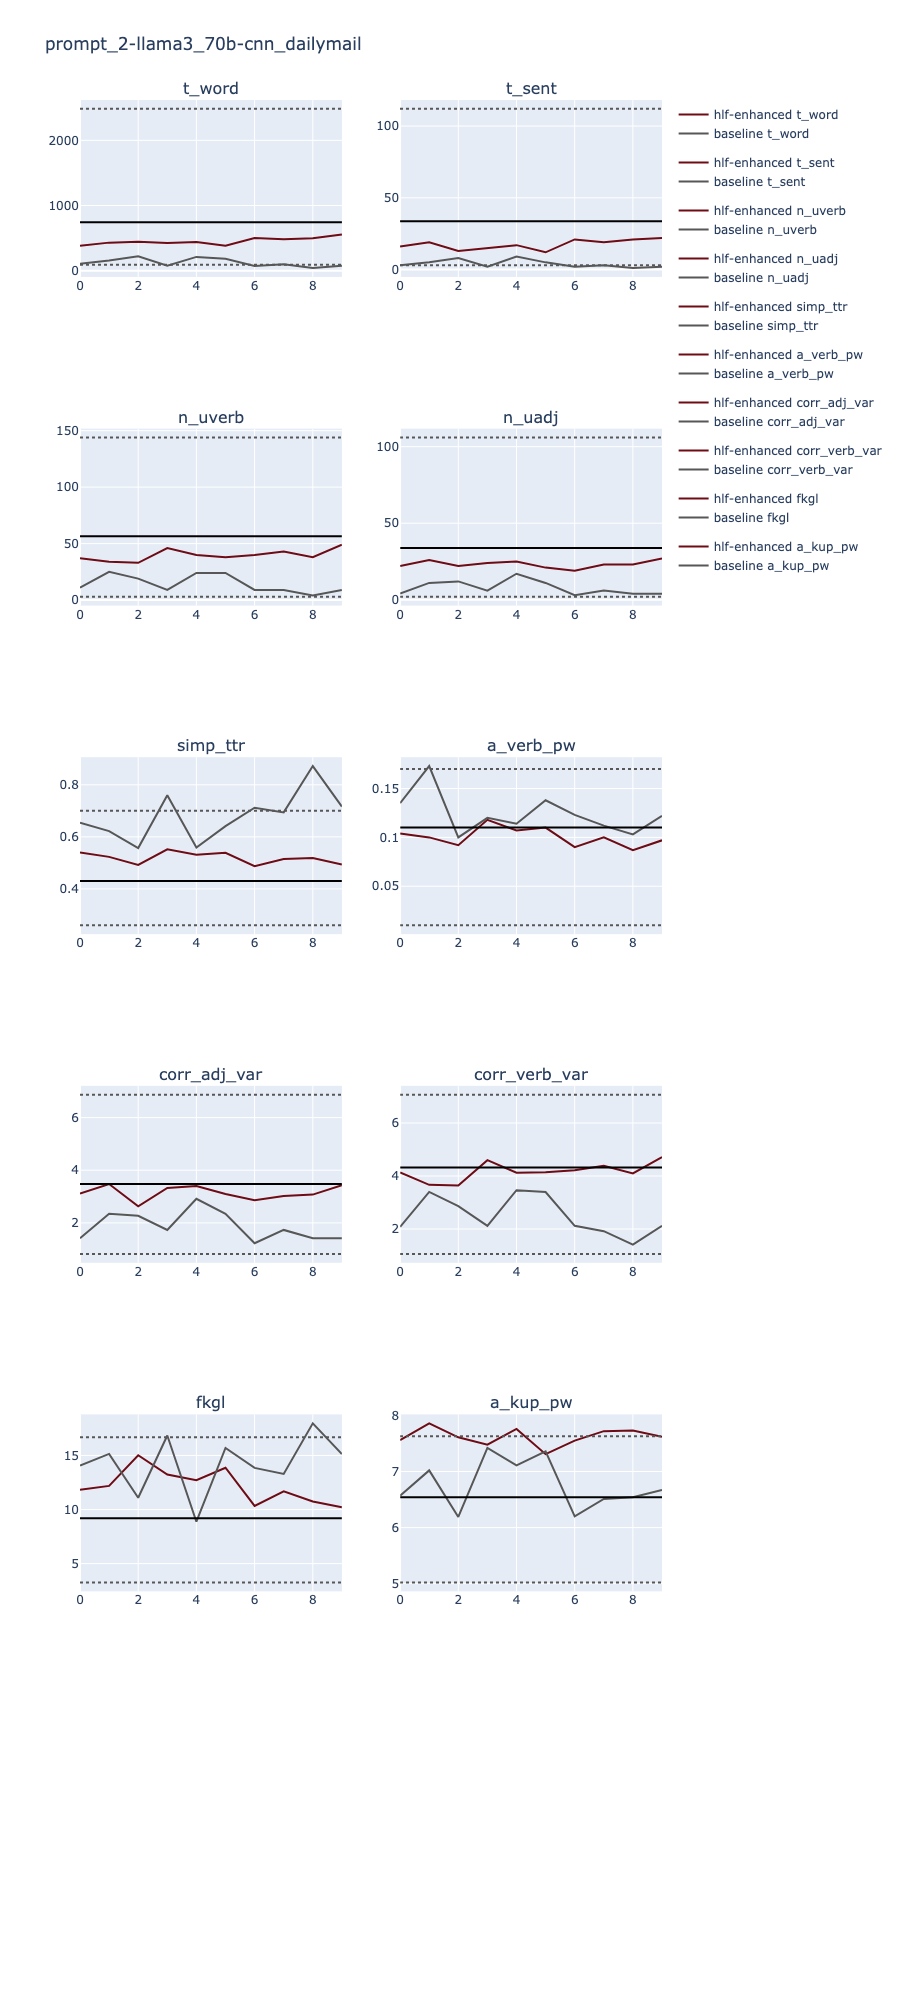
\includegraphics[width=\textwidth,height=0.9\textheight,scale=1]{plots/prompt_2_ifd/prompt_2-llama3_70b-cnn_dailymail/prompt_2-llama3_70b-cnn_dailymail.png}
    \caption{Llama3 on CNN Corpus\\Prompt With Examples\\Input from Corpus}\label{fig:llama3_70b-prompt2-cnn-ifd}
\end{figure*}
\begin{figure*}[ht]
    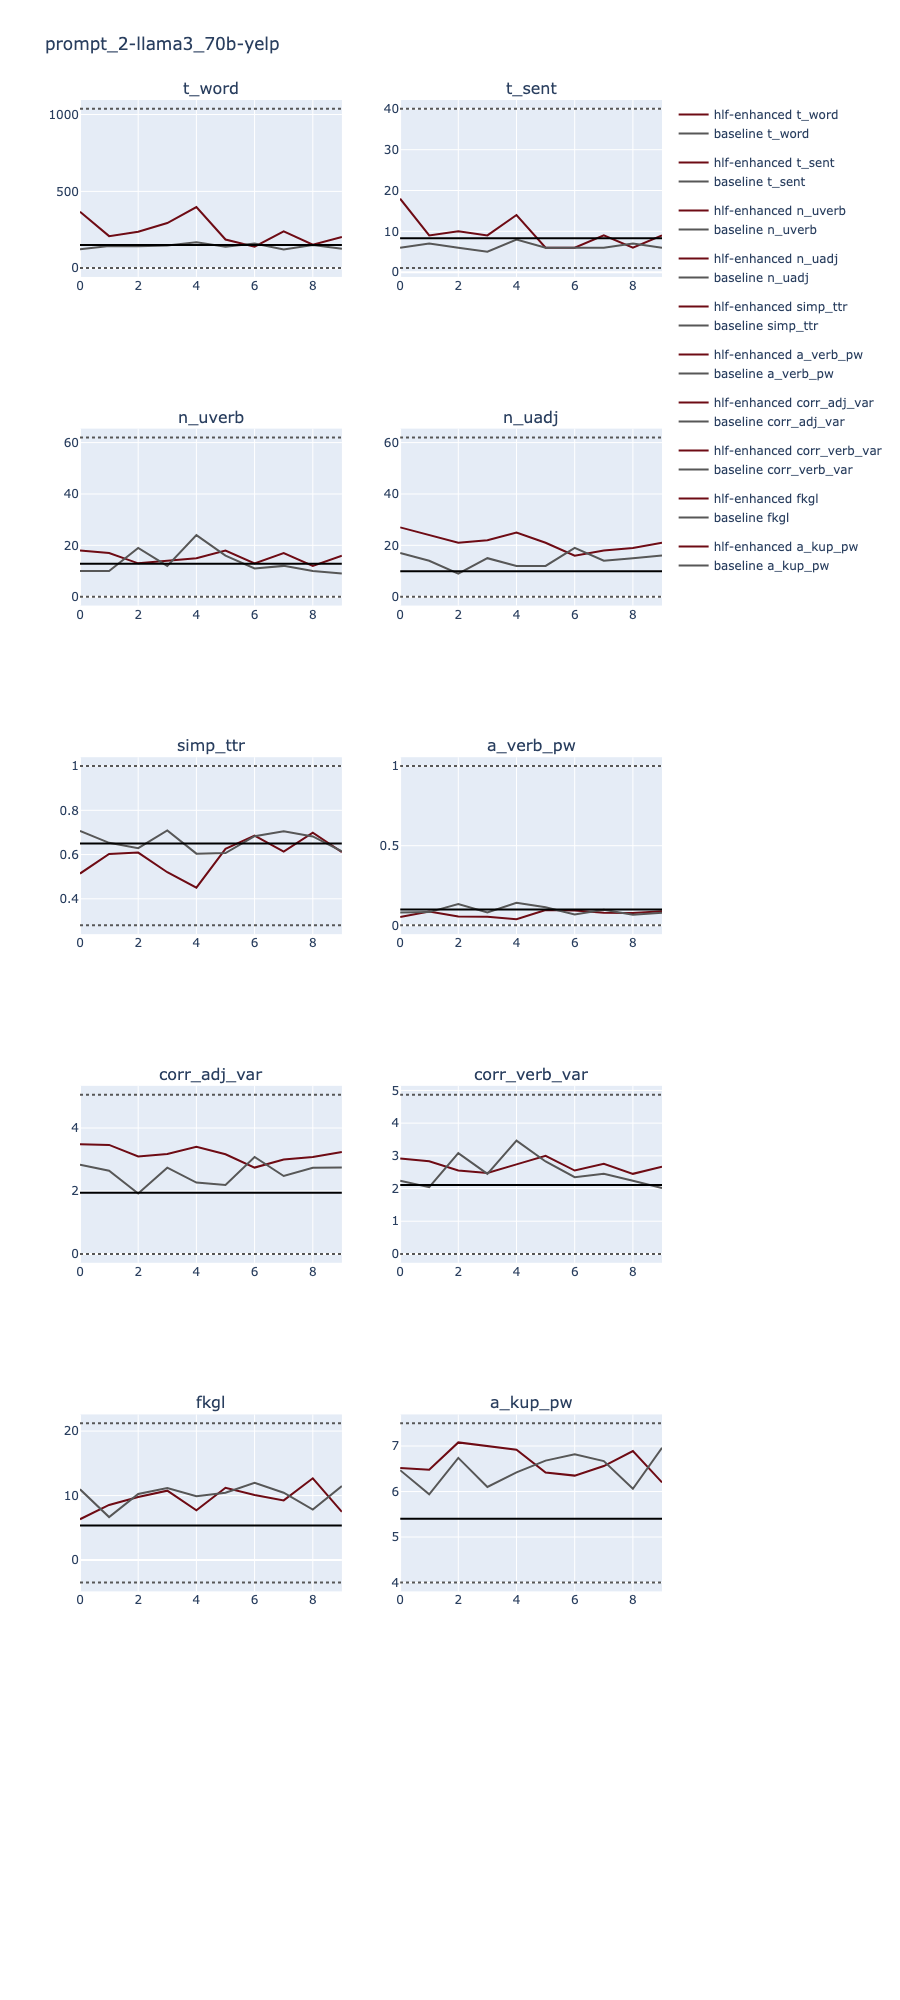
\includegraphics[width=\textwidth,height=0.9\textheight,scale=1]{plots/prompt_2_ifd/prompt_2-llama3_70b-yelp/prompt_2-llama3_70b-yelp.png}
    \caption{Llama3 on Yelp Corpus\\Prompt With Examples\\Input from Corpus}\label{fig:llama3_70b-prompt2-yelp-ifd}
\end{figure*}

\Cref{fig:llama3_70b-prompt1-cnn,fig:llama3_70b-prompt1-yelp,fig:llama3_70b-prompt2-cnn,fig:llama3_70b-prompt2-yelp,fig:llama3_70b-prompt2-cnn-ifd,fig:llama3_70b-prompt2-yelp-ifd}
show the experiment results for the Claude 3 Opus large language model.

\subsection{Command R+}

\begin{figure*}[ht]
    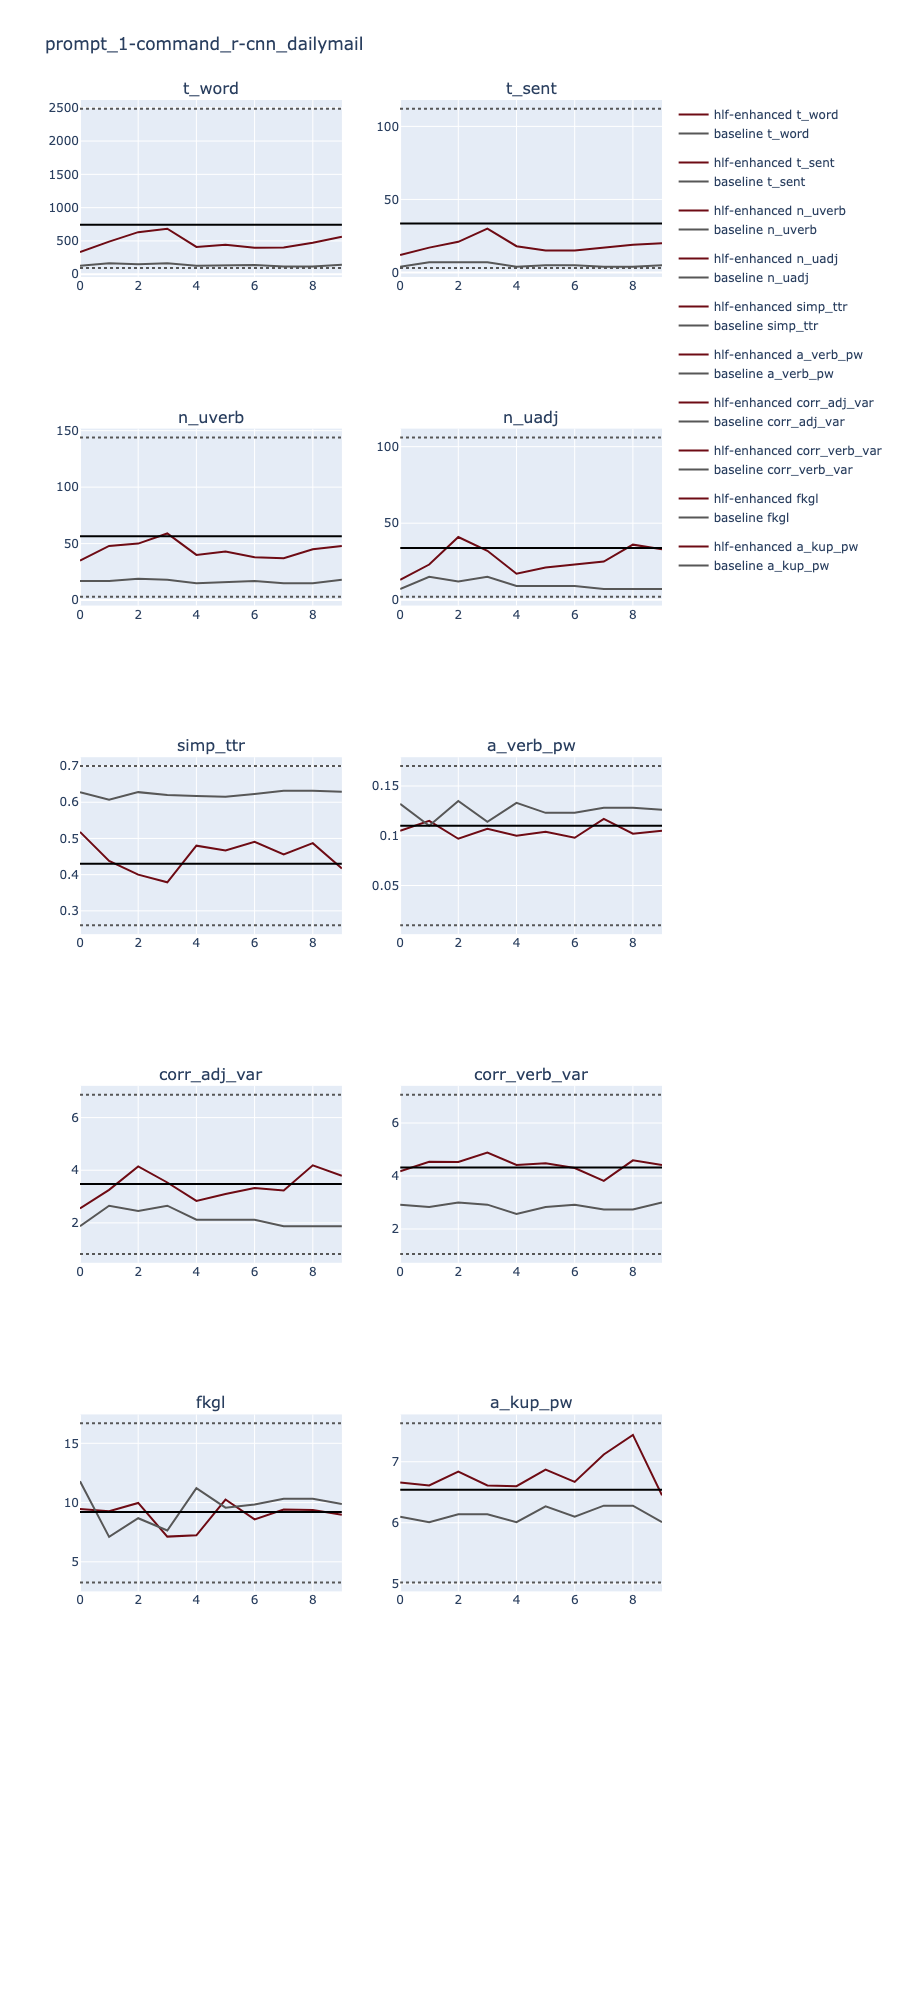
\includegraphics[width=\textwidth,height=0.9\textheight,scale=1]{plots/prompt_1/prompt_1-command_r-cnn_dailymail/prompt_1-command_r-cnn_dailymail.png}
    \caption{Command R on CNN Corpus\\Prompt Without Examples}\label{fig:command_r-prompt1-cnn}
\end{figure*}
\begin{figure*}[ht]
    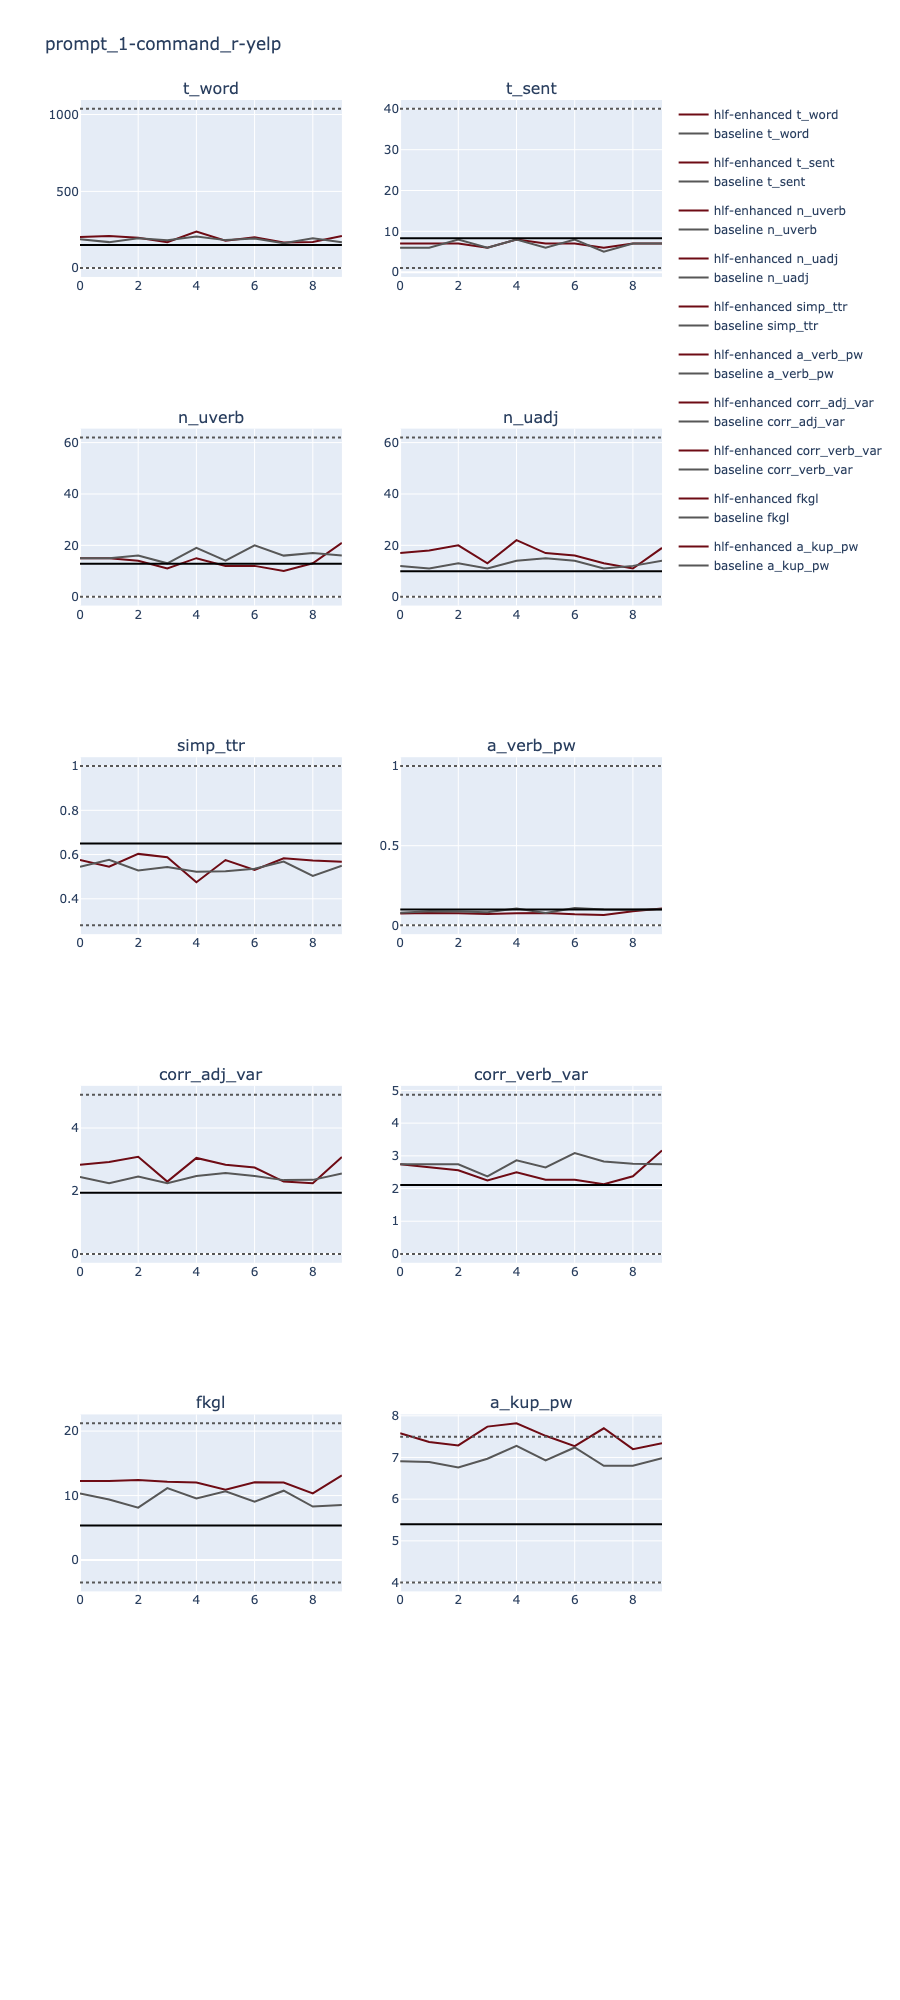
\includegraphics[width=\textwidth,height=0.9\textheight,scale=1]{plots/prompt_1/prompt_1-command_r-yelp/prompt_1-command_r-yelp.png}
    \caption{Command R on Yelp Corpus\\Prompt Without Examples}\label{fig:command_r-prompt1-yelp}
\end{figure*}
\begin{figure*}[ht]
    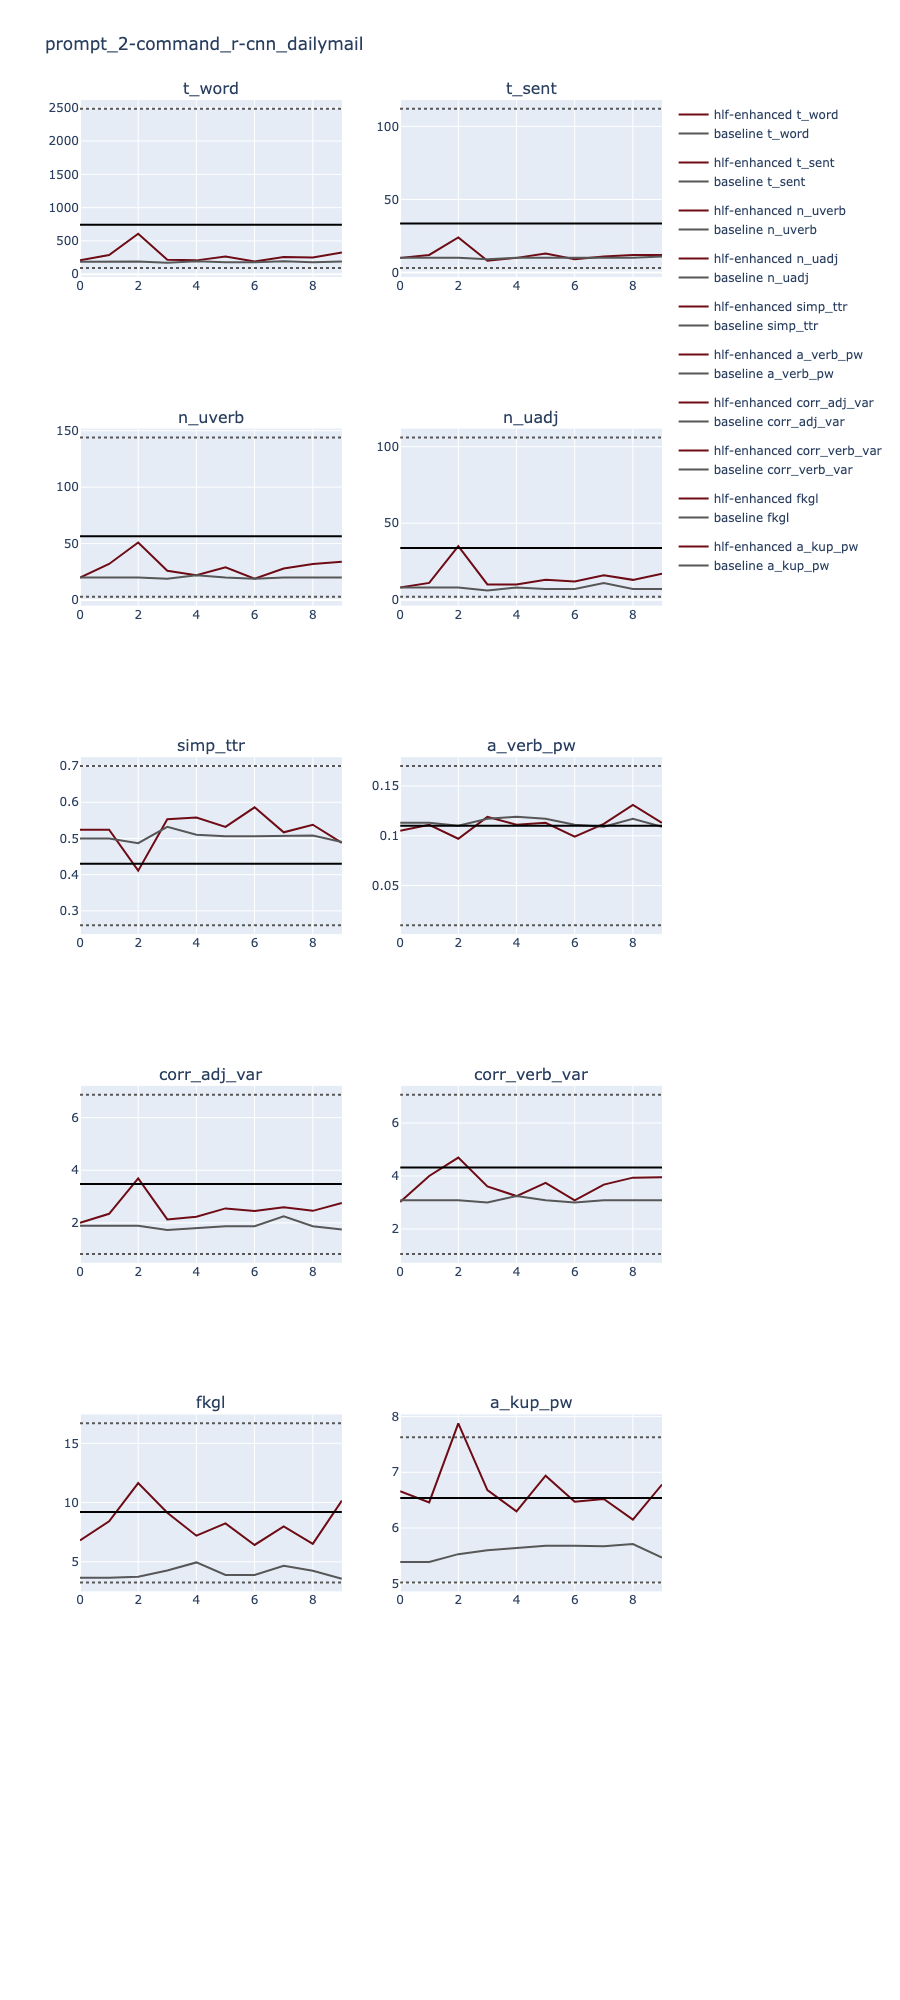
\includegraphics[width=\textwidth,height=0.9\textheight,scale=1]{plots/prompt_2/prompt_2-command_r-cnn_dailymail/prompt_2-command_r-cnn_dailymail.png}
    \caption{Command R on CNN Corpus\\Prompt With Examples\\Extraneous Input}\label{fig:command_r-prompt2-cnn}
\end{figure*}
\begin{figure*}[ht]
    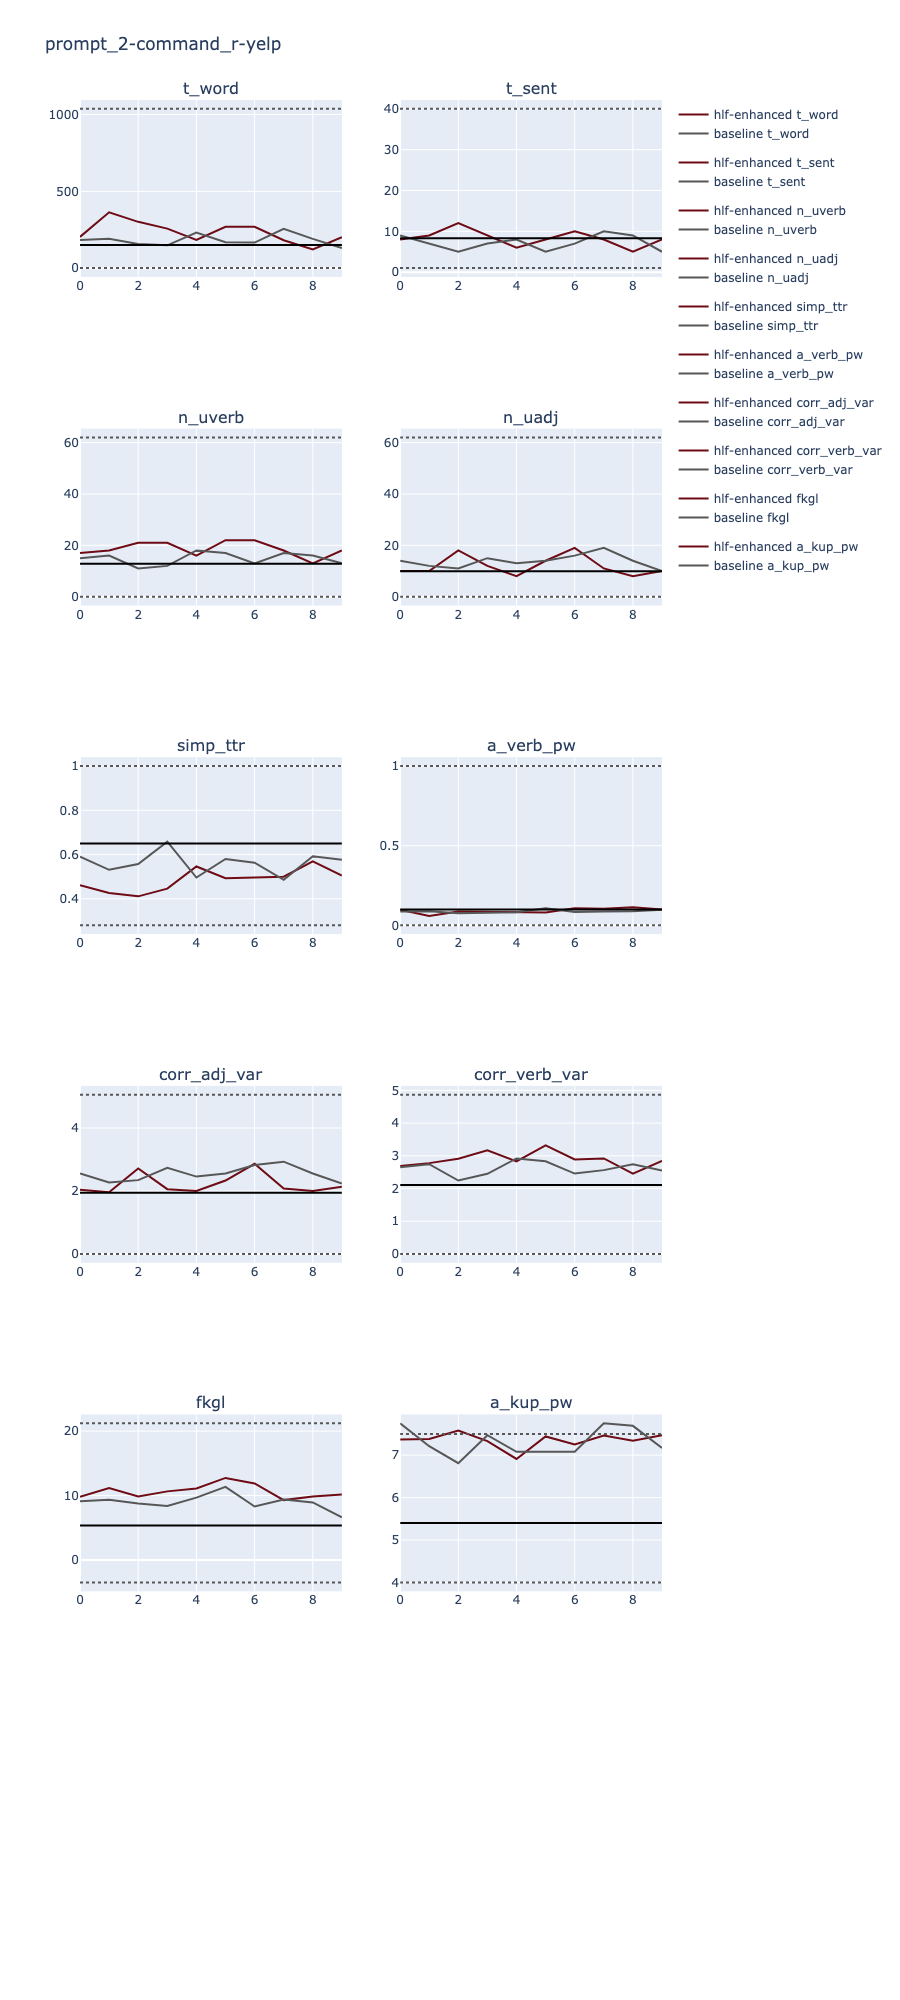
\includegraphics[width=\textwidth,height=0.9\textheight,scale=1]{plots/prompt_2/prompt_2-command_r-yelp/prompt_2-command_r-yelp.png}
    \caption{Command R on Yelp Corpus\\Prompt With Examples\\Extraneous Input}\label{fig:command_r-prompt2-yelp}
\end{figure*}
\begin{figure*}[ht]
    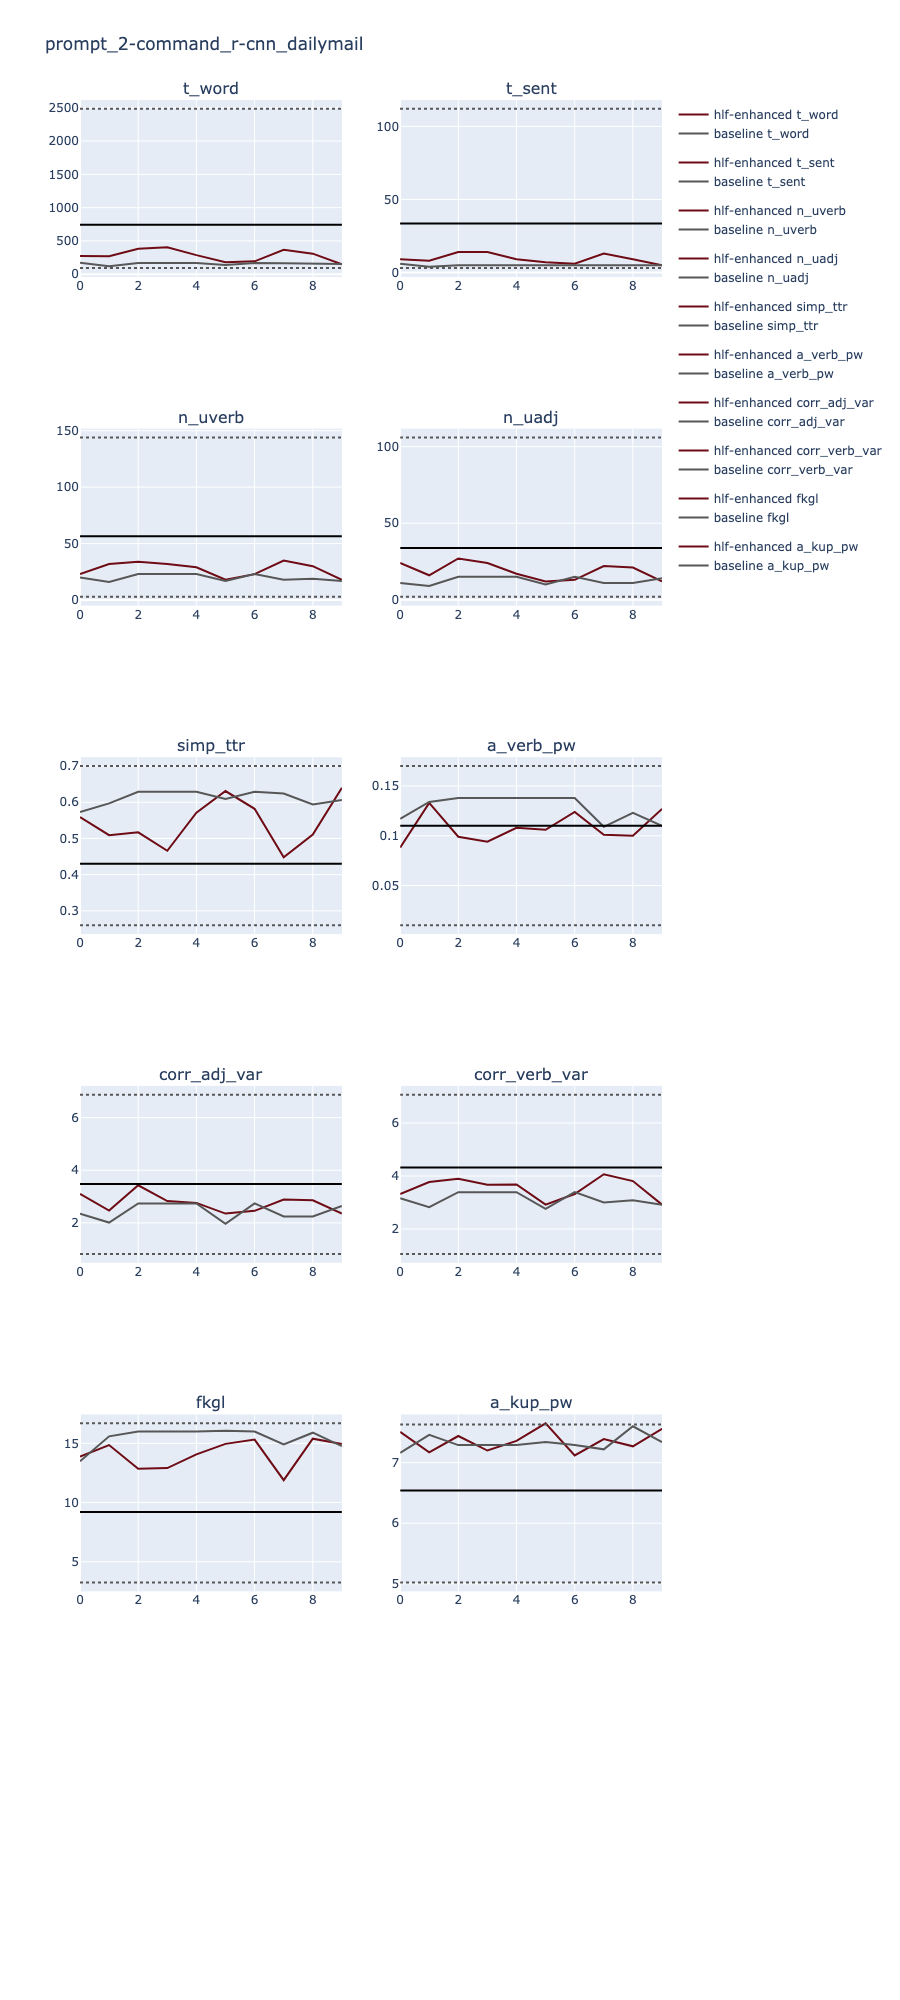
\includegraphics[width=\textwidth,height=0.9\textheight,scale=1]{plots/prompt_2_ifd/prompt_2-command_r-cnn_dailymail/prompt_2-command_r-cnn_dailymail.png}
    \caption{Command R on CNN Corpus\\Prompt With Examples\\Input from Corpus}\label{fig:command_r-prompt2-cnn-ifd}
\end{figure*}
\begin{figure*}[ht]
    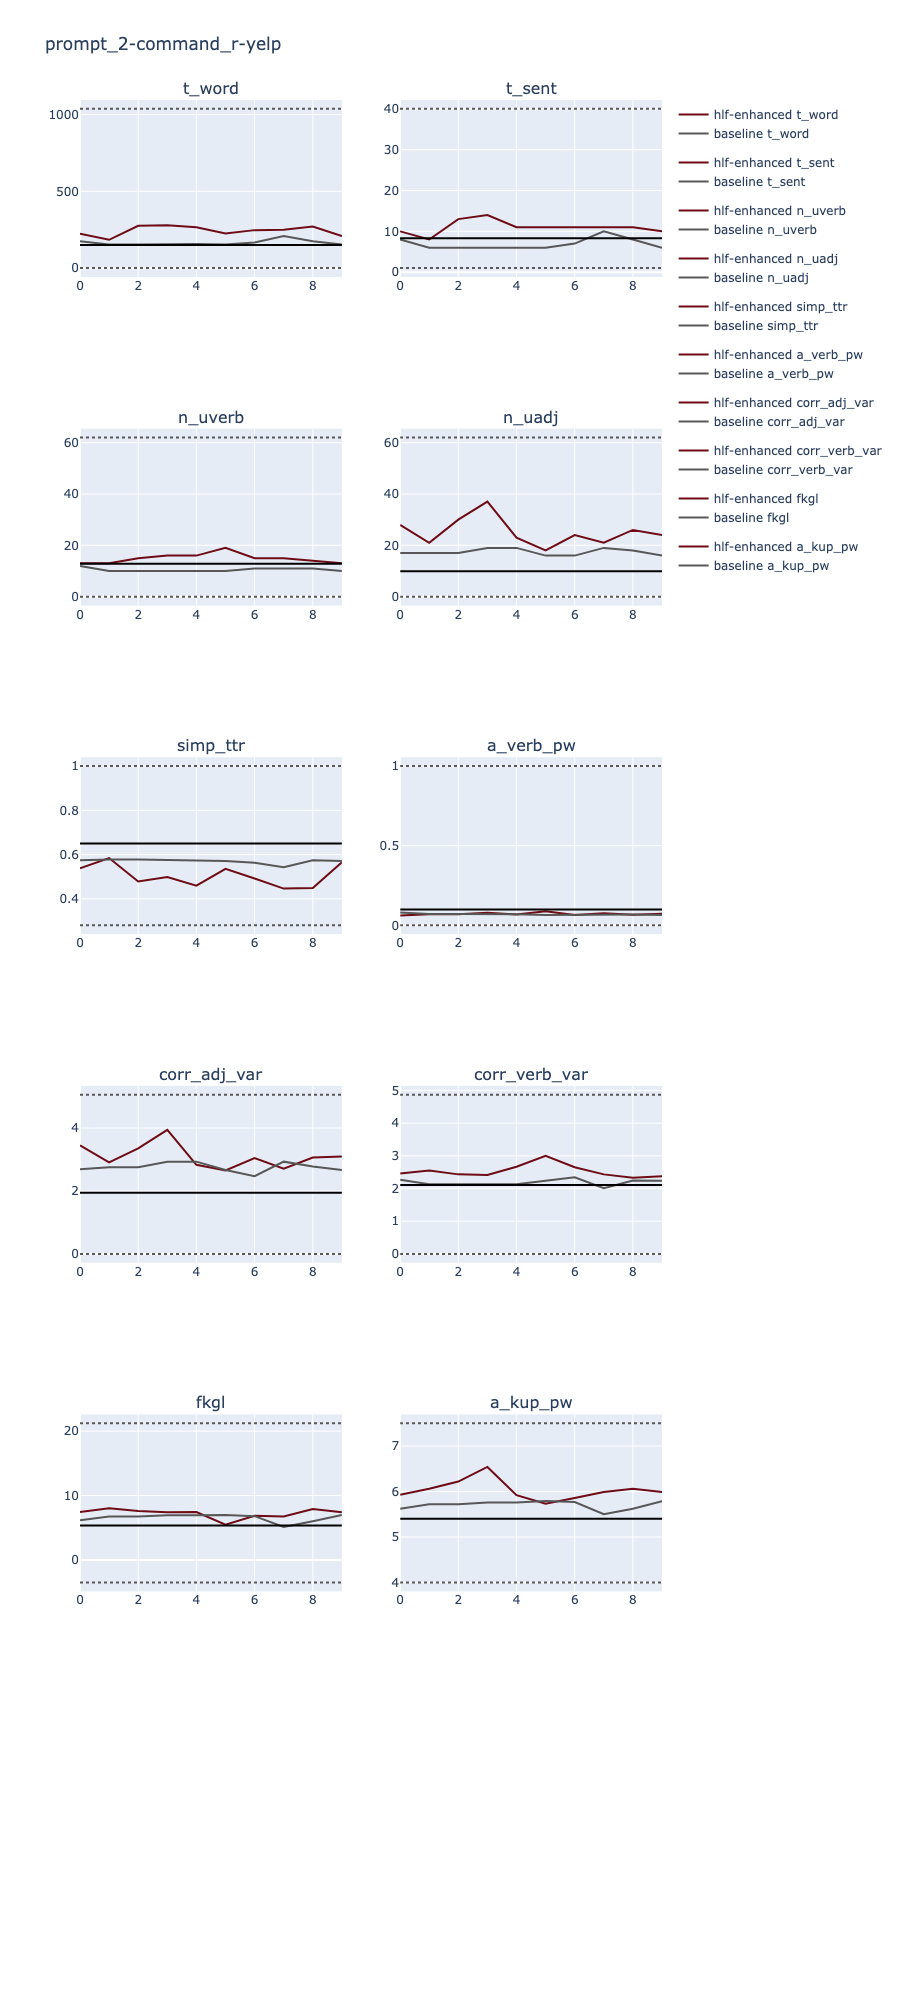
\includegraphics[width=\textwidth,height=0.9\textheight,scale=1]{plots/prompt_2_ifd/prompt_2-command_r-yelp/prompt_2-command_r-yelp.png}
    \caption{Command R on Yelp Corpus\\Prompt With Examples\\Input from Corpus}\label{fig:command_r-prompt2-yelp-ifd}
\end{figure*}

\Cref{fig:command_r-prompt1-cnn,fig:command_r-prompt1-yelp,fig:command_r-prompt2-cnn,fig:command_r-prompt2-yelp,fig:command_r-prompt2-cnn-ifd,fig:command_r-prompt2-yelp-ifd}
show the experiment results for the Claude 3 Opus large language model.

\end{document}